% !TeX spellcheck = en-US
% !TeX encoding = utf8
% !TeX program = pdflatex
% !BIB program = biber
% -*- coding:utf-8 mod:LaTeX -*-


% vv  scroll down to line 200 for content  vv


\let\ifdeutsch\iftrue
\let\ifenglish\iffalse


% EN: This file is loaded before the \documentclass command in the main document

% EN: The following package allows \\ at the title page
%     For more information see https://github.com/latextemplates/scientific-thesis-cover/issues/4
\RequirePackage{kvoptions-patch}

\ifenglisch
  \PassOptionsToClass{numbers=noenddot}{scrbook}
\else
  %()Aus scrguide.pdf - der Dokumentation von KOMA-Script)
  %Nach DUDEN steht in Gliederungen, in denen ausschließlich arabische Ziffern für die Nummerierung
  %verwendet werden, am Ende der Gliederungsnummern kein abschließender Punkt
  %(siehe [DUD96, R3]). Wird hingegen innerhalb der Gliederung auch mit römischen Zahlen
  %oder Groß- oder Kleinbuchstaben gearbeitet, so steht am Ende aller Gliederungsnummern ein
  %abschließender Punkt (siehe [DUD96, R4])
  \PassOptionsToClass{numbers=autoendperiod}{scrbook}
\fi

% Warns about outdated packages and missing caption declarations
% See https://www.ctan.org/pkg/nag
\RequirePackage[l2tabu, orthodox]{nag}

%DE: Neue deutsche Trennmuster
%    Siehe http://www.ctan.org/pkg/dehyph-exptl und http://projekte.dante.de/Trennmuster/WebHome
%    Nur für pdflatex, nicht für lualatex
\RequirePackage{ifluatex}
\ifluatex
  % do not load anything
\else
  \ifdeutsch
    \RequirePackage[ngerman=ngerman-x-latest]{hyphsubst}
  \fi
\fi

\documentclass[
  %
  %ngerman, %%% Add if you write in German.
  %
  % fontsize=11pt is the standard
  a4paper,  % Standard format - only KOMAScript uses paper=a4 - https://tex.stackexchange.com/a/61044/9075
  twoside,  % we are optimizing for both screen and two-side printing. So the page numbers will jump, but the content is configured to stay in the middle (by using the geometry package)
  bibliography=totoc,
  %               idxtotoc,   %Index ins Inhaltsverzeichnis
  %               liststotoc, %List of X ins Inhaltsverzeichnis, mit liststotocnumbered werden die Abbildungsverzeichnisse nummeriert
  headsepline,
  cleardoublepage=empty,
  parskip=half,
  %               draft    % um zu sehen, wo noch nachgebessert werden muss - wichtig, da Bindungskorrektur mit drin
  draft=false
]{scrbook}
% !TeX encoding = utf8
% -*- coding:utf-8 mod:LaTeX -*-

% EN: This file includes basic packages and sets options. The order of package
%     loading is important

% DE: In dieser Datei werden zuerst die benoetigten Pakete eingebunden und
%     danach diverse Optionen gesetzt. Achtung Reihenfolge ist entscheidend!


% EN: Styleguide:
% - English comments are prefixed with "EN", German comments are prefixed with "DE"
% - Prefixed headings define the language for the subsequent paragraphs
% - It is tried to organize packages in blocks. Bocks are separated by two empty lines.

% DE: Styleguide:
%
% Ein sehr kleiner Styleguide. Packages werden in Blöcken organisiert.
% Zwischen zwei Blöcken sind 2 Leerzeilen!


% EN: Enable copy and paste of text from the PDF
%     Only required for pdflatex. It "just works" in the case of lualatex.
%     mmap enables mathematical symbols, but does not work with the newtx font set
%     See: https://tex.stackexchange.com/a/64457/9075
%     Other solutions outlined at http://goemonx.blogspot.de/2012/01/pdflatex-ligaturen-und-copynpaste.html and http://tex.stackexchange.com/questions/4397/make-ligatures-in-linux-libertine-copyable-and-searchable
%     Trouble shooting outlined at https://tex.stackexchange.com/a/100618/9075

\ifluatex
\else
  \usepackage{cmap}
\fi


% EN: File encoding
% DE: Codierung
%     Wir sind im 21 Jahrhundert, utf-8 löst so viele Probleme.
%
% Mit UTF-8 funktionieren folgende Pakete nicht mehr. Bitte beachten!
%   * fancyvrb mit §
%   * easylist -> http://www.ctan.org/tex-archive/macros/latex/contrib/easylist/
\ifluatex
  % EN: See https://tex.stackexchange.com/a/158517/9075
  %     Not required, because of usage of fontspec package
  %\usepackage[utf8]{luainputenc}
\else
  \usepackage[utf8]{inputenc}
\fi


% DE: Parallelbetrieb tex4ht und pdflatex

\makeatletter
\@ifpackageloaded{tex4ht}{
  \def\iftex4ht{\iftrue}
}{
  \def\iftex4ht{\iffalse}
}
\makeatother


% EN: Mathematics
% DE: Mathematik
%
% DE: Viele Mathematik-Sachen. Siehe https://texdoc.net/pkg/amsmath
%
% EN: Options must be passed this way, otherwise it does not work with glossaries
% DE: fleqn (=Gleichungen linksbündig platzieren) funktioniert nicht direkt. Es muss noch ein Patch gemacht werden:
\PassOptionsToPackage{fleqn,leqno}{amsmath}
%
% DE: amsmath Muss nicht mehr geladen werden, da es von newtxmath automatisch geladen wird
% \usepackage{amsmath}


%% EN: Fonts
%% DE: Schriften
%%
%% !!! If you change the font, be sure that words such as "workflow" can
%% !!! still be copied from the PDF. If this is not the case, you have
%% !!! to use glyphtounicode. See comment at cmap package


% EN: Times Roman for all text
\ifluatex
  % source: Second proposed fix from the following answer: https://tex.stackexchange.com/a/394137
  \usepackage[no-math]{fontspec}
  \setmainfont{TeXGyreTermes-Regular}[
       BoldFont       = TeXGyreTermes-Bold ,
       ItalicFont     = TeXGyreTermes-Italic ,
       BoldItalicFont = TeXGyreTermes-BoldItalic,
       NFSSFamily     = ntxtlf]
  \setsansfont{TeX Gyre Heros Regular}[
       Scale=.9,
       BoldFont       = TeX Gyre Heros Bold,
       ItalicFont     = TeX Gyre Heros Italic,
       BoldItalicFont = TeX Gyre Heros BoldItalic]
  \setmonofont[StylisticSet={1,3},Scale=.9]{inconsolata}
  \RequirePackage{newtxmath}
\else
  \RequirePackage{newtxtext}
  \RequirePackage{newtxmath}
  % EN: looks good with times, but no equivalent for lualatex found,
  %     therefore replaced with inconsolata
  %\RequirePackage[zerostyle=b,scaled=.9]{newtxtt}
  \RequirePackage[varl,scaled=.9]{inconsolata}
\fi

% EN: Fallback font - if the subsequent font packages do not define a font (e.g., monospaced)
%     This is the modern package for "Computer Modern".
%     In case this gets activated, one has to switch from cmap package to glyphtounicode (in the case of pdflatex)
% DE: Fallback-Schriftart
%\usepackage[%
%    rm={oldstyle=false,proportional=true},%
%    sf={oldstyle=false,proportional=true},%
%    tt={oldstyle=false,proportional=true,variable=true},%
%    qt=false%
%]{cfr-lm}

% EN: Headings are typset in Helvetica (which is similar to Arial)
% DE: Schriftart fuer die Ueberschriften - ueberschreibt lmodern
%\usepackage[scaled=.95]{helvet}

% DE: Für Schreibschrift würde tun, muss aber nicht
%\usepackage{mathrsfs} %  \mathscr{ABC}

% EN: Font for the main text
% DE: Schriftart fuer den Fliesstext - ueberschreibt lmodern
%     Linux Libertine, siehe http://www.linuxlibertine.org/
%     Packageparamter [osf] = Minuskel-Ziffern
%     rm = libertine im Brottext, Linux Biolinum NICHT als serifenlose Schrift, sondern helvet (von oben) beibehalten
%\usepackage[rm]{libertine}

% EN: Alternative Font: Palantino. It is recommeded by Prof. Ludewig for German texts
% DE: Alternative Schriftart: Palantino, Packageparamter [osf] = Minuskel-Ziffern
%     Bitte nur in deutschen Texten
%\usepackage{mathpazo} %ftp://ftp.dante.de/tex-archive/fonts/mathpazo/ - Tipp aus DE-TEX-FAQ 8.2.1

% DE: Schriftart fuer Programmcode - ueberschreibt lmodern
%     Falls auskommentiert, wird die Standardschriftart lmodern genommen
%     Fuer schreibmaschinenartige Schluesselwoerter in den Listings - geht bei alten Installationen nicht, da einige Fontshapes (<>=) fehlen
%\usepackage[scaled=.92]{luximono}
%\usepackage{courier}
% DE: BeraMono als Typewriter-Schrift, Tipp von http://tex.stackexchange.com/a/71346/9075
%\usepackage[scaled=0.83]{beramono}

% EN: backticks (`) are rendered as such in verbatim environments.
%     See following links for details:
%     - https://tex.stackexchange.com/a/341057/9075
%     - https://tex.stackexchange.com/a/47451/9075
%     - https://tex.stackexchange.com/a/166791/9075
\usepackage{upquote}

% DE: Symbole
%
%\usepackage[geometry]{ifsym} % \BigSquare
%\usepackage{mathabx}
%\usepackage{stmaryrd} %fuer \ovee, \owedge, \otimes
%\usepackage{marvosym} %fuer \Writinghand %patched to not redefine \Rightarrow
%\usepackage{mathrsfs} %mittels \mathscr{} schoenen geschwungenen Buchstaben erzeugen
%\usepackage{calrsfs} %\mathcal{} ein bisserl dickeren buchstaben erzeugen - sieht net so gut aus.
%durch mathpazo ist das schon definiert

%
%\usepackage{amssymb}

% EN: For \texttrademark{}
\usepackage{textcomp}

% EN: name-clashes von marvosym und mathabx vermeiden:
\def\delsym#1{%
  %  \expandafter\let\expandafter\origsym\expandafter=\csname#1\endcsname
  %  \expandafter\let\csname orig#1\endcsname=\origsym
  \expandafter\let\csname#1\endcsname=\relax
}

%\usepackage{pifont}
%\usepackage{bbding}
%\delsym{Asterisk}
%\delsym{Sun}\delsym{Mercury}\delsym{Venus}\delsym{Earth}\delsym{Mars}
%\delsym{Jupiter}\delsym{Saturn}\delsym{Uranus}\delsym{Neptune}
%\delsym{Pluto}\delsym{Aries}\delsym{Taurus}\delsym{Gemini}
%\delsym{Rightarrow}
%\usepackage{mathabx} - Ueberschreibt leider zu viel - und die \le-Zeichen usw. sehen nicht gut aus!


% EN: Modern font encoding
%     Has to be loaded AFTER any font packages. See https://tex.stackexchange.com/a/2869/9075.
\ifluatex
\else
  \usepackage[T1]{fontenc}
\fi
%


% EN: Character protrusion and font expansion. See http://www.ctan.org/tex-archive/macros/latex/contrib/microtype/
% DE: Optischer Randausgleich und Grauwertkorrektur

\usepackage[
  babel=true, % EN: Enable language-specific kerning. Take language-settings from the languge of the current document (see Section 6 of microtype.pdf)
  expansion=alltext,
  protrusion=alltext-nott, % EN: Ensure that at listings, there is no change at the margin of the listing
  final % EN: Always enable microtype, even if in draft mode. This helps finding bad boxes quickly.
        %     In the standard configuration, this template is always in the final mode, so this option only makes a difference if "pros" use the draft mode
]{microtype}


% EN: \texttt{test -- test} keeps the "--" as "--" (and does not convert it to an en dash)
\DisableLigatures{encoding = T1, family = tt* }

% DE: fuer microtype
% DE: tracking=true muss als Parameter des microtype-packages mitgegeben werden
% DE: Deaktiviert, da dies bei Algorithmen seltsam aussieht

%\DeclareMicrotypeSet*[tracking]{my}{ font = */*/*/sc/* }%
%\SetTracking{ encoding = *, shape = sc }{ 45 }
% DE: Hier wird festgelegt,
%     dass alle Passagen in Kapitälchen automatisch leicht
%     gesperrt werden.
%     Quelle: http://homepage.ruhr-uni-bochum.de/Georg.Verweyen/pakete.html
%    Deaktiviert, da sonst "BPEL", "BPMN" usw. wirklich komisch aussehen.
%     Macht wohl nur bei geisteswissenschaftlichen Arbeiten Sinn.


% EN: amsmath teaks


% EN: Fixes bugs in AMS math
%     Corrently conflicts with unicode-math
% \usepackage{mathtools}

%\numberwithin{equation}{section}
%\renewcommand{\theequation}{\thesection.\Roman{equation}}

% EN: work-around ams-math problem with align and 9 -> 10. Does not work with glossaries, No visual changes.
%\addtolength\mathindent{1em}


% EN: For theorems, replacement for amsthm
\usepackage[amsmath,hyperref]{ntheorem}
\theorempreskipamount 2ex plus1ex minus0.5ex
\theorempostskipamount 2ex plus1ex minus0.5ex
\theoremstyle{break}
\newtheorem{definition}{Definition}[section]


% CTAN: https://ctan.org/pkg/lccaps
% Doc: http://texdoc.net/pkg/lccaps
%
% Required for DE/EN \initialism
\usepackage{lccaps}


% EN: Defintion of colors. Argument "hyperref" is not used as we do not want to change border colors of links: Links are not colored anymore.
% DE: Farbdefinitionen
\usepackage[dvipsnames]{xcolor}


% EN: Required for custom acronyms/glossaries style.
%     Left aligned Columns in tables with fixed width.
%     See http://tex.stackexchange.com/questions/91566/syntax-similar-to-centering-for-right-and-left
\usepackage{ragged2e}


% DE: Wichtig, ansonsten erscheint "No room for a new \write"
\usepackage{scrwfile}


% EN: Support for language-specific hyphenation
% DE: Neue deutsche Rechtschreibung und Literatur statt "Literature"
%     Die folgende Einstellung ist der Nachfolger von ngerman.sty
\ifdeutsch
  % DE: letzte Sprache ist default, Einbindung von "american" ermöglicht \begin{otherlanguage}{amercian}...\end{otherlanguage} oder \foreignlanguage{american}{Text in American}
  %     Siehe auch http://tex.stackexchange.com/a/50638/9075
  \usepackage[american,main=ngerman]{babel}
  % Ein "abstract" ist eine "Kurzfassung", keine "Zusammenfassung"
  \addto\captionsngerman{%
    \renewcommand\abstractname{Kurzfassung}%
  }
  \ifluatex
    % EN: conditionally disable ligatures. See https://github.com/latextemplates/scientific-thesis-template/issues/54
    %     for a discussion
    \usepackage[ngerman]{selnolig}
  \fi
\else
  % EN: Set English as language and allow to write hyphenated"=words
  %     `american`, `english` and `USenglish` are synonyms for babel package (according to https://tex.stackexchange.com/questions/12775/babel-english-american-usenglish).
  %      "english" has to go last to set it as default language
  \usepackage[english]{babel}
  % EN: Hint by http://tex.stackexchange.com/a/321066/9075 -> enable "= as dashes
  \addto\extrasenglish{\languageshorthands{ngerman}\useshorthands{"}}
  \ifluatex
    % EN: conditionally disable ligatures. See https://github.com/latextemplates/scientific-thesis-template/issues/54
    %     for a discussion
    \usepackage[english]{selnolig}
  \fi
\fi
%


% EN: For easy quotations: \enquote{text}
%     This package is very smart when nesting is applied, otherwise textcmds (see below) provides a shorter command
%     Note that this package results in a warning when it is loaded before minted (actually fvextra).
% DE: Anführungszeichen
%     Zitate in \enquote{...} setzen, dann werden automatisch die richtigen Anführungszeichen verwendet.
%     Dieses package erzeugt eine Warnung, wenn es vor minted (genauer fvextra) geladen wird.
\usepackage{csquotes}


% EN: For even easier quotations: \qq{text}.
%     Is not smart in the case of nesting, but good enough for the most cases
\usepackage{textcmds}
\ifdeutsch
  % EN: German quotes are different. So do not use the English quotes, but the ones provided by the csquotes package.
  \renewcommand{\qq}[1]{\enquote{#1}}
\fi


% EN: extended enumarations
% DE: erweitertes Enumerate
\usepackage{paralist}


% DE: Gestaltung der Kopf- und Fußteilen

\usepackage[automark]{scrlayer-scrpage}

\automark[section]{chapter}
\setkomafont{pageheadfoot}{\normalfont\sffamily}
\setkomafont{pagenumber}{\normalfont\sffamily}

% DE: funktioniert nicht: Alle Linien sind hier weg
%\setheadsepline[.4pt]{.4pt}


% DE: Intelligentes Leerzeichen um hinter Abkürzungen die richtigen Abstände zu erhalten, auch leere.
%     Siehe commands.tex \gq{}
\usepackage{xspace}
% DE: Macht \xspace und \enquote kompatibel
\makeatletter
\xspaceaddexceptions{\grqq \grq \csq@qclose@i \} }
\makeatother


\newcommand{\eg}{e.\,g.,\ }
\newcommand{\ie}{i.\,e.,\ }


% EN: introduce \powerset - hint by http://matheplanet.com/matheplanet/nuke/html/viewtopic.php?topic=136492&post_id=997377
\DeclareFontFamily{U}{MnSymbolC}{}
\DeclareSymbolFont{MnSyC}{U}{MnSymbolC}{m}{n}
\DeclareFontShape{U}{MnSymbolC}{m}{n}{
  <-6>    MnSymbolC5
  <6-7>   MnSymbolC6
  <7-8>   MnSymbolC7
  <8-9>   MnSymbolC8
  <9-10>  MnSymbolC9
  <10-12> MnSymbolC10
  <12->   MnSymbolC12%
}{}
\DeclareMathSymbol{\powerset}{\mathord}{MnSyC}{180}


% EN: Package for the appendix
% DE: Anhang
\usepackage{appendix}
%[toc,page,title,header]
%


% EN: Graphics
% DE: Grafikeinbindungen
%
% EN: The parameter "pdftex" is not required
\usepackage{graphicx}
\graphicspath{{\getgraphicspath}}
\newcommand{\getgraphicspath}{graphics/}


% EN: Enables inclusion of SVG graphics - 1:1 approach
%    This is NOT the approach of https://ctan.org/pkg/svg-inkscape,
%     which allows text in SVG to be typeset using LaTeX
%     We just include the SVG as is.
\usepackage{epstopdf}
\epstopdfDeclareGraphicsRule{.svg}{pdf}{.pdf}{%
  inkscape -z -D --file=#1 --export-pdf=\OutputFile
}


% EN: Enables inclusion of SVG graphics - text-rendered-with-LaTeX-approach
%     This is the approach of https://ctan.org/pkg/svg-inkscape,
\newcommand{\executeiffilenewer}[3]{%
  \IfFileExists{#2}
  {
    %\message{file #2 exists}
    \ifnum\pdfstrcmp{\pdffilemoddate{#1}}%
      {\pdffilemoddate{#2}}>0%
      {\immediate\write18{#3}}
    \else
      {%\message{file up to date #2}
      }
    \fi%
  }{
    %\message{file #2 doesn't exist}
    %\message{argument: #3}
    %\immediate\write18{echo "test" > xoutput.txt}
    \immediate\write18{#3}
  }
}
\newcommand{\includesvg}[1]{%
  \executeiffilenewer{#1.svg}{#1.pdf}%
  {
    inkscape -z -D --file=\getgraphicspath#1.svg %
    --export-pdf=\getgraphicspath#1.pdf --export-latex}%
  \input{\getgraphicspath#1.pdf_tex}%
}


% EN: Enable typesetting values with SI units.
%\ifdeutsch
%  \usepackage[mode=text,group-four-digits]{siunitx}
%  \sisetup{locale=DE}
%\else
%  \usepackage[mode=text,group-four-digits,group-separator={,}]{siunitx}
%  \sisetup{locale=US}
%\fi


% EN: Extensions for tables
% DE: Tabellenerweiterungen
\usepackage{array} %increases tex's buffer size and enables ``>'' in tablespecs
\usepackage{longtable}
\usepackage{dcolumn} %Aligning numbers by decimal points in table columns
\ifdeutsch
  \newcolumntype{d}[1]{D{.}{,}{#1}}
\else
  \newcolumntype{d}[1]{D{.}{.}{#1}}
\fi
\setlength{\extrarowheight}{1pt}


% DE: Eine Zelle, die sich über mehrere Zeilen erstreckt.
%     Siehe Beispieltabelle in Kapitel 2
\usepackage{multirow}


% DE: Fuer Tabellen mit Variablen Spaltenbreiten
\usepackage{tabularx}
%\usepackage{tabulary}


% EN: Links behave as they should. Enables "\url{...}" for URL typesettings.
%     Allow URL breaks also at a hyphen, even though it might be confusing: Is the "-" part of the address or just a hyphen?
%     See https://tex.stackexchange.com/a/3034/9075.
% DE: Links verhalten sich so, wie sie sollen
%     Zeilenumbrüche bei URLs auch bei Bindestrichen erlauben, auch wenn es verwirrend sein könnte: Gehört der Bindestrich zur URL oder ist es ein Trennstrich?
%     Siehe https://tex.stackexchange.com/a/3034/9075.
\usepackage[hyphens]{url}
%
%  EN: When activated, use text font as url font, not the monospaced one.
%      For all options see https://tex.stackexchange.com/a/261435/9075.
% \urlstyle{same}
%
% EN: Hint by http://tex.stackexchange.com/a/10419/9075.
\makeatletter
\g@addto@macro{\UrlBreaks}{\UrlOrds}
\makeatother


% DE: Index über Begriffe, Abkürzungen
%\usepackage{makeidx} makeidx ist out -> http://xindy.sf.net verwenden


% DE: lustiger Hack fuer das Abkuerzungsverzeichnis
%     nach latex durchlauf folgendes ausfuehren
%     makeindex ausarbeitung.nlo -s nomencl.ist -o ausarbeitung.nls
%     danach nochmal latex
%\usepackage{nomencl}
%    \let\abk\nomenclature %Deutsche Ueberschrift setzen
%          \renewcommand{\nomname}{List of Abbreviations}
%        %Punkte zw. Abkuerzung und Erklaerung
%          \setlength{\nomlabelwidth}{.2\hsize}
%          \renewcommand{\nomlabel}[1]{#1 \dotfill}
%        %Zeilenabstaende verkleinern
%          \setlength{\nomitemsep}{-\parsep}
%    \makenomenclature


% EN: Logic for TeX - enables if-then-else in commands
% DE: Logik für TeX
%     FÜr if-then-else @ commands.tex
\usepackage{ifthen}


% EN: Code Listings
% DE: Listings
\usepackage{listings}
\lstset{language=XML,
  showstringspaces=false,
  extendedchars=true,
  basicstyle=\footnotesize\ttfamily,
  commentstyle=\slshape,
  % DE: Original: \rmfamily, damit werden die Strings im Quellcode hervorgehoben. Zusaetzlich evtl.: \scshape oder \rmfamily durch \ttfamily ersetzen. Dann sieht's aus, wie bei fancyvrb
  stringstyle=\ttfamily,
  breaklines=true,
  breakatwhitespace=true,
  % EN: alternative: fixed
  columns=flexible,
  numbers=left,
  numberstyle=\tiny,
  basewidth=.5em,
  xleftmargin=.5cm,
  % aboveskip=0mm, %DE: deaktivieren, falls man lstlistings direkt als floating object benutzt (\begin{lstlisting}[float,...])
  % belowskip=0mm, %DE: deaktivieren, falls man lstlistings direkt als floating object benutzt (\begin{lstlisting}[float,...])
  captionpos=b
}

\ifluatex
\else
  % EN: Enable UTF-8 support - see https://tex.stackexchange.com/q/419327/9075
  \usepackage{listingsutf8}
  \lstset{inputencoding=utf8/latin1}
\fi

\ifdeutsch
  \renewcommand{\lstlistlistingname}{Verzeichnis der Listings}
\fi


% EN: Alternative to listings could be fancyvrb. Can be used together.
% DE: Alternative zu Listings ist fancyvrb. Kann auch beides gleichzeitig benutzt werden.
\usepackage{fancyvrb}
%
% EN: Font size for the normal text
% DE: Groesse fuer den Fliesstext. Falls deaktiviert: \normalsize
%\fvset{fontsize=\small}
%
% DE: Somit kann im Text ganz einfach §verbatim§ text gesetzt werden.
%     Disabled, because UTF-8 does not work any more and lualatex causes issues
%\DefineShortVerb{\§}
%
% EN: Shrink font size of listings
\RecustomVerbatimEnvironment{Verbatim}{Verbatim}{fontsize=\footnotesize}
\RecustomVerbatimCommand{\VerbatimInput}{VerbatimInput}{fontsize=\footnotesize}
%
% EN: Hack for fancyvrb based on http://newsgroups.derkeiler.com/Archive/Comp/comp.text.tex/2008-12/msg00075.html
%     Change of the solution: \Vref somehow collidated with cleveref/varioref as the output of \Vref{} was "Abschnitt 4.3 auf Seite 85"; therefore changed to \myVref -- so completely removed
%     See https://tex.stackexchange.com/q/132420/9075 for more information.
\newcommand{\Vlabel}[1]{\label[line]{#1}\hypertarget{#1}{}}
\newcommand{\lref}[1]{\hyperlink{#1}{\FancyVerbLineautorefname~\ref*{#1}}}


% EN: Tunings of captions for floats, listings, ...
% DE: Bildunterschriften bei floats genauso formatieren wie bei Listings
%     Anpassung wird unten bei den newfloat-Deklarationen vorgenommen
%     https://www.ctan.org/pkg/caption2 is superseeded by this package.
\usepackage{caption}


% EN: Provides rotating figures, where the PDF page is also turned
% DE: Ermoeglicht es, Abbildungen um 90 Grad zu drehen
%     Alternatives Paket: rotating Allerdings wird hier nur das Bild gedreht, während bei lscape auch die PDF-Seite gedreht wird.
%     Das Paket lscape dreht die Seite auch nicht
\usepackage{pdflscape}


% EN: Required for proper environments of fancyvrb and lstlistings
%    There is also the newfloat pacakge (recommended by minted), but we currently have no expericene with that
% DE: Wird für fancyvrb und für lstlistings verwendet
\usepackage{float}
%
% EN: Alternative to float package
%\usepackage{floatrow}
% DE: zustäzlich für den Paramter [H] = Floats WIRKLICH da wo sie deklariert wurden paltzieren - ganz ohne Kompromisse
%     floatrow ist der Nachfolger von float
%     Allerdings macht floatrow in manchen Konstellationen Probleme. Deshalb ist das Paket deaktiviert.
%
% EN: See http://www.tex.ac.uk/cgi-bin/texfaq2html?label=floats
% DE: floats IMMER nach einer Referenzierung platzieren
%\usepackage{flafter}


% EN: Put footnotes below floats
%     Source: https://tex.stackexchange.com/a/32993/9075
\usepackage{stfloats}
\fnbelowfloat


% EN: For nested figures
% DE: Fuer Abbildungen innerhalb von Abbildungen
%     Ersetzt die Pakete subfigure und subfig - siehe https://tex.stackexchange.com/a/13778/9075
\usepackage[hypcap=true]{subcaption}


% EN: Extended support for footnotes
% DE: Fußnoten
%
%\usepackage{dblfnote}  %Zweispaltige Fußnoten
%
% Keine hochgestellten Ziffern in der Fußnote (KOMA-Script-spezifisch):
%\deffootnote[1.5em]{0pt}{1em}{\makebox[1.5em][l]{\bfseries\thefootnotemark}}
%
% Abstand zwischen Fußnoten vergrößern:
%\setlength{\footnotesep}{.85\baselineskip}
%
% EN: Following command disables the separting line of the footnote
% DE: Folgendes Kommando deaktiviert die Trennlinie zur Fußnote
%\renewcommand{\footnoterule}{}
%
\addtolength{\skip\footins}{\baselineskip} % Abstand Text <-> Fußnote
%
% Fußnoten immer ganz unten auf einer \raggedbottom-Seite
% fnpos kommt aus dem yafoot package
\usepackage{fnpos}
\makeFNbelow
\makeFNbottom


% EN: Variable page heights
% DE: Variable Seitenhöhen zulassen
\raggedbottom


% DE: Falls die Seitenzahl bei einer Referenz auf eine Abbildung nur dann angegeben werden soll,
%     falls sich die Abbildung nicht auf der selben Seite befindet...
\iftex4ht
  %tex4ht does not work well with vref, therefore we emulate vref behavior
  \newcommand{\vref}[1]{\ref{#1}}
\else
  \ifdeutsch
    \usepackage[ngerman]{varioref}
  \else
    \usepackage{varioref}
  \fi
\fi


% EN: More beautiful tables if one uses \toprule, \midrule, \bottomrule
% DE: Noch schoenere Tabellen als mit booktabs mit http://www.zvisionwelt.de/downloads.html
\usepackage{booktabs}
%
%\usepackage[section]{placeins}


% EN: Graphs and Automata
%
% TODO: Since version 3.0 (2013-10-01), it supports pdflatex via the auto-pst-pdf package
%       Requires -shell-escape
%\usepackage{gastex}


%\usepackage{multicol}

% DE: kollidiert mit diplomarbeit.sty
%\usepackage{setspace}


% DE: biblatex statt bibtex
\usepackage[
  backend       = biber, %biber does not work with 64x versions alternative: bibtex8
  %minalphanames only works with biber backend
  sortcites     = true,
  bibstyle      = numeric,
  citestyle     = numeric,
  giveninits    = false,
  useprefix     = false, %"von, van, etc." will be printed, too. See below.
  minnames      = 1,
  minalphanames = 3,
  maxalphanames = 4,
  maxbibnames   = 99,
  maxcitenames  = 2,
  natbib        = true,
  eprint        = true,
  url           = true,
  doi           = true,
  isbn          = true,
  backref       = false]{biblatex}

% enable more breaks at URLs. See https://tex.stackexchange.com/a/134281.
\setcounter{biburllcpenalty}{7000}
\setcounter{biburlucpenalty}{8000}

\bibliography{bibliography}
\addbibresource[datatype=bibtex]{bibliography.bib}

%Do not put "vd" in the label, but put it at "\citeauthor"
%Source: http://tex.stackexchange.com/a/30277/9075
\makeatletter
\AtBeginDocument{\toggletrue{blx@useprefix}}
\AtBeginBibliography{\togglefalse{blx@useprefix}}
\makeatother

%Thin spaces between initials
%http://tex.stackexchange.com/a/11083/9075
\renewrobustcmd*{\bibinitdelim}{\,}

%Keep first and last name together in the bibliography
%http://tex.stackexchange.com/a/196192/9075
\renewcommand*\bibnamedelimc{\addnbspace}
\renewcommand*\bibnamedelimd{\addnbspace}

%Replace last "and" by comma in bibliography
%See http://tex.stackexchange.com/a/41532/9075
\AtBeginBibliography{%
  \renewcommand*{\finalnamedelim}{\addcomma\space}%
}

\ifdeutsch
  \DefineBibliographyStrings{ngerman}{
    backrefpage  = {zitiert auf S\adddot},
    backrefpages = {zitiert auf S\adddot},
    andothers    = {et\ \addabbrvspace al\adddot},
    %Tipp von http://www.mrunix.de/forums/showthread.php?64665-biblatex-Kann-%DCberschrift-vom-Inhaltsverzeichnis-nicht-%E4ndern&p=293656&viewfull=1#post293656
    bibliography = {Literaturverzeichnis}
  }
\fi

% EN: enable hyperlinked author names when using \citeauthor
%     source: http://tex.stackexchange.com/a/75916/9075
\DeclareCiteCommand{\citeauthor}
{\boolfalse{citetracker}%
  \boolfalse{pagetracker}%
  \usebibmacro{prenote}}
{\ifciteindex
  {\indexnames{labelname}}
  {}%
  \printtext[bibhyperref]{\printnames{labelname}}}
{\multicitedelim}
{\usebibmacro{postnote}}

% EN: natbib compatibility
%\newcommand{\citep}[1]{\cite{#1}}
%\newcommand{\citet}[1]{\citeauthor{#1} \cite{#1}}
% EN: Beginning of sentence - analogous to cleveref - important for names such as "zur Muehlen"
%\newcommand{\Citep}[1]{\cite{#1}}
%\newcommand{\Citet}[1]{\Citeauthor{#1} \cite{#1}}

% DE: Blindtext. Paket "blindtext" ist fortgeschritterner als "lipsum" und kann auch Mathematik im Text (http://texblog.org/2011/02/26/generating-dummy-textblindtext-with-latex-for-testing/)
%     kantlipsum (https://www.ctan.org/tex-archive/macros/latex/contrib/kantlipsum) ist auch ganz nett, aber eben auch keine Mathematik
%     Wird verwendet, um etwas Text zu erzeugen, um eine volle Seite wegen Layout zu sehen.
\usepackage[math]{blindtext}


% EN: Make LaTeX logos available by commands. E.g., \lualatex
%     Disabled, because currently causes \not= already defined
%\usepackage{dtk-logos}

% quick replacement:
\newcommand{\LuaLaTeX}{Lua\LaTeX\xspace}
\newcommand{\lualatex}{\LuaLaTeX}

% DE: Neue Pakete bitte VOR hyperref einbinden. Insbesondere bei Verwendung des
%     Pakets "index" wichtig, da sonst die Referenzierung nicht funktioniert.
%     Für die Indizierung selbst ist unter http://xindy.sourceforge.net
%     ein gutes Tool zu erhalten.
%     Hier also neue packages einbinden.
% EN: Add new packages at this place.


% EN: Provides hyperlinks
%     Option "unicode" fixes umlauts in the PDF bookmarks - see https://tex.stackexchange.com/a/338770/9075
%
% DE: Erlaubt Hyperlinks im Dokument.
%     Alle Optionen nach \hypersetup verschoben, sonst crash
%     Siehe auch: "Praktisches LaTeX" - www.itp.uni-hannover.de/~kreutzm
\usepackage[unicode]{hyperref}


% EN: Define colors
% DE: Da es mit KOMA 3 und xcolor zu Problemen mit den global Options kommt MÜSSEN die Optionen so gesetzt werden.
%     Eigene Farbdefinitionen ohne die Namen des xcolor packages
\definecolor{darkblue}{rgb}{0,0,.5}
\definecolor{black}{rgb}{0,0,0}


% EN: Define color of links and more
\hypersetup{
  % have both title and number hyperlinking to content
  linktoc=all,
  bookmarksnumbered=true,
  bookmarksopen=true,
  bookmarksopenlevel=1,
  breaklinks=true,
  colorlinks=true,
  pdfstartview=Fit,
  pdfpagelayout=SinglePage, % DE: Alterntaive: TwoPageRight -- zweiseitige Darstellung: ungerade Seiten rechts im PDF-Viewer - siehe auch http://tex.stackexchange.com/a/21109/9075
  %pdfencoding=utf8, % EN: This is probably the same as passing the option "unicode" at \usepackage{hyperref}
  filecolor=black,
  urlcolor=black,
  linkcolor=black,
  citecolor=black
}

\ifenglish
    %\renewcommand{\sectionautorefname}{Section}
    %\renewcommand{\subsectionautorefname}{Section}
    %\renewcommand{\subsubsectionautorefname}{Section}
    \defcaptionname*{english}{\chapterautorefname}{Chapter}
    \defcaptionname*{english}{\sectionautorefname}{Section}
    \defcaptionname*{english}{\subsectionautorefname}{Section}
    \defcaptionname*{english}{\subsubsectionautorefname}{Section}
    \defcaptionname*{english}{\Listingautorefname}{Listing}
    \defcaptionname*{english}{\Algorithmusautorefname}{Algorithmus}
\else
\fi

% EN: Abbreviations - has to be loaded after hyperref
% DE: Abkürzungsverzeichnis - muss nach hyperref geladen werden
%
% DE: siehe http://www.dickimaw-books.com/cgi-bin/faq.cgi?action=view&categorylabel=glossaries#glsnewwriteexceeded
\usepackage[acronym,indexonlyfirst,nomain]{glossaries}
\ifdeutsch
  \addto\captionsngerman % DE: siehe https://tex.stackexchange.com/a/154566
  {%
    \renewcommand*{\acronymname}{Abkürzungsverzeichnis}
  }
\else
  \renewcommand*{\acronymname}{List of Abbreviations}
\fi
\renewcommand*{\glsgroupskip}{}
%
% EN: Removed Glossarie as a table as a quick fix to get the template working again
%     See http://tex.stackexchange.com/questions/145579/how-to-print-acronyms-of-glossaries-into-a-table
%
\makenoidxglossaries


% EN: Extensions for references inside the document (\cref{fig:sample}, ...)
% DE: cleveref für cref statt autoref, da cleveref auch bei Definitionen funktioniert
%\usepackage[capitalise,nameinlink,noabbrev]{cleveref}
%\ifdeutsch
%  \crefname{table}{Tabelle}{Tabellen}
%  \Crefname{table}{Tabelle}{Tabellen}
%  \crefname{figure}{\figurename}{\figurename}
%  \Crefname{figure}{Abbildung}{Abbildungen}
%  \crefname{equation}{Gleichung}{Gleichungen}
%  \Crefname{equation}{Gleichung}{Gleichungen}
%  \crefname{theorem}{Theorem}{Theoreme}
%  \Crefname{theorem}{Theorem}{Theoreme}
%  \crefname{listing}{\lstlistingname}{\lstlistingname}
%  \Crefname{listing}{Listing}{Listings}
%  \crefname{section}{Abschnitt}{Abschnitte}
%  \Crefname{section}{Abschnitt}{Abschnitte}
%  \crefname{paragraph}{Abschnitt}{Abschnitte}
%  \Crefname{paragraph}{Abschnitt}{Abschnitte}
%  \crefname{subparagraph}{Abschnitt}{Abschnitte}
%  \Crefname{subparagraph}{Abschnitt}{Abschnitte}
%\else
%  \crefname{listing}{\lstlistingname}{\lstlistingname}
%  \Crefname{listing}{Listing}{Listings}
%\fi


% DE: Zur Darstellung von Algorithmen
%     Algorithm muss nach hyperref geladen werden
\usepackage[chapter]{algorithm}
\usepackage[]{algpseudocode}


% DE: Links auf Gleitumgebungen springen nicht zur Beschriftung,
%     Doc: http://mirror.ctan.org/tex-archive/macros/latex/contrib/oberdiek/hypcap.pdf
%     sondern zum Anfang der Gleitumgebung
\usepackage[all]{hypcap}


% DE: Deckblattstyle
%
\ifdeutsch
  \PassOptionsToPackage{language=german}{scientific-thesis-cover}
\else
  \PassOptionsToPackage{language=english}{scientific-thesis-cover}
\fi


% EN: Bugfixes packages
%\usepackage{fixltx2e} %Fuer neueste LaTeX-Installationen nicht mehr benoetigt - bereinigte einige Ungereimtheiten, die auf Grund von Rueckwaertskompatibilitaet beibahlten wurden.
%\usepackage{mparhack} %Fixt die Position von marginpars (die in DAs selten bis gar nicht gebraucht werden}
%\usepackage{ellipsis} %Fixt die Abstaende vor \ldots. Wird wohl auch nicht benoetigt.


% EN: Settings for captions of floats
% DE: Formatierung der Beschriftungen
%
\captionsetup{
  format=hang,
  labelfont=bf,
  justification=justified,
  %single line captions should be centered, multiline captions justified
  singlelinecheck=true
}


% EN: New float environments for listings and algorithms
%
% \floatstyle{ruled} % TODO: enabled or disabled causes no change - listings and algorithms are always ruled
%
\newfloat{Listing}{tbp}{code}[chapter]
%\crefname{Listing}{Listing}{Listings}

\newfloat{Algorithmus}{tbp}{alg}[chapter]
\ifdeutsch
  %\crefname{Algorithmus}{Algorithmus}{Algorithmus}
\else
  %\crefname{Algorithmus}{Algorithm}{Algorithms}
  \floatname{Algorithmus}{Algorithm}
\fi



% EN: Various chapter styles
% DE: unterschiedliche Chapter-Styles
%     u.a. Paket fncychap

% Andere Kapitelueberschriften
% falls einem der Standard von KOMA nicht gefaellt...
% Falls man zurück zu KOMA moechte, dann muss jede der vier folgenden Moeglichkeiten deaktiviert sein.

%\usepackage[Sonny]{fncychap}

%\usepackage[Bjarne]{fncychap}

%\usepackage[Lenny]{fncychap}

%DE: Zur Aktivierung eines der folgenden Möglichkeiten ein Paar von "\iffalse" und "\fi" auskommentieren

\iffalse
  \usepackage[Bjarne]{fncychap}
  \ChNameVar{\Large\sf} \ChNumVar{\Huge} \ChTitleVar{\Large\sf}
  \ChRuleWidth{0.5pt} \ChNameUpperCase
\fi

\iffalse
  \usepackage[Rejne]{fncychap}
  \ChNameVar{\centering\Huge\rm\bfseries}
  \ChNumVar{\Huge}
  \ChTitleVar{\centering\Huge\rm}
  \ChNameUpperCase
  \ChTitleUpperCase
  \ChRuleWidth{1pt}
\fi

\iffalse
  \usepackage{fncychap}
  \ChNameUpperCase
  \ChTitleUpperCase
  \ChNameVar{\raggedright\normalsize} %\rm
  \ChNumVar{\bfseries\Large}
  \ChTitleVar{\raggedright\Huge}
  \ChRuleWidth{1pt}
\fi

\iffalse
  \usepackage[Bjornstrup]{fncychap}
  \ChNumVar{\fontsize{76}{80}\selectfont\sffamily\bfseries}
  \ChTitleVar{\raggedright\Large\sffamily\bfseries}
\fi

% EN: Complete different chapter style - self made

% Innen drin kann man dann noch zwischen
%   * serifenloser Schriftart (eingestellt)
%   * serifenhafter Schriftart (wenn kein zusaetzliches Kommando aktiviert ist) und
%   * Kapitälchen wählen
\iffalse
  \makeatletter
  %\def\thickhrulefill{\leavevmode \leaders \hrule height 1ex \hfill \kern \z@}

  %Fuer Kapitel mit Kapitelnummer
  \def\@makechapterhead#1{%
    \vspace*{10\p@}%
    {\parindent \z@ \raggedright \reset@font
      %Default-Schrift: Serifenhaft (gut fuer englische Dokumente)
      %A) Fuer serifenlose Schrift:
      \fontfamily{phv}\selectfont
      %B) Fuer Kapitaelchen:
      %\fontseries{m}\fontshape{sc}\selectfont
      %C) Fuer ganz "normale" Schrift:
      %\normalfont
      %
      \Large \@chapapp{} \thechapter
      \par\nobreak\vspace*{10\p@}%
      \interlinepenalty\@M
      {\Huge\bfseries\baselineskip3ex
        %Fuer Kapitaelchen folgende Zeile aktivieren:
        %\fontseries{m}\fontshape{sc}\selectfont
        #1\par\nobreak}
      \vspace*{10\p@}%
      \makebox[\textwidth]{\hrulefill}%    \hrulefill alone does not work
      \par\nobreak
      \vskip 40\p@
    }}

  %Fuer Kapitel ohne Kapitelnummer (z.B. Inhaltsverzeichnis)
  \def\@makeschapterhead#1{%
    \vspace*{10\p@}%
    {\parindent \z@ \raggedright \reset@font
      \normalfont \vphantom{\@chapapp{} \thechapter}
      \par\nobreak\vspace*{10\p@}%
      \interlinepenalty\@M
      {\Huge \bfseries %
        %Default-Schrift: Serifenhaft (gut fuer englische Dokumente)
        %A) Fuer serifenlose Schrift folgende Zeile aktivieren:
        \fontfamily{phv}\selectfont
        %B) Fuer Kapitaelchen folgende Zeile aktivieren:
        %\fontseries{m}\fontshape{sc}\selectfont
        #1\par\nobreak}
      \vspace*{10\p@}%
      \makebox[\textwidth]{\hrulefill}%    \hrulefill does not work
      \par\nobreak
      \vskip 40\p@
    }}
  %
  \makeatother
\fi


% DE: Minitoc-Einstellungen
%\dominitoc
%\renewcommand{\mtctitle}{Inhaltsverzeichnis dieses Kapitels}


% EN: Nicer paragraph line placement:
%     - Disable single lines at the start of a paragraph (Schusterjungen)
%     - Disable single lines at the end of a paragraph (Hurenkinder)
%     Normally, this is clubpenalty and widowpenalty, but using a package, it feels more non-hacky
\usepackage[all,defaultlines=3]{nowidow}
%
\displaywidowpenalty = 10000


% EN: Try to get rid of "overfull hbox" things and let text flow batter
%     See also
%       - http://groups.google.de/group/de.comp.text.tex/browse_thread/thread/f97da71d90442816/f5da290593fd647e?lnk=st&q=tolerance+emergencystretch&rnum=5&hl=de#f5da290593fd647e
%       - http://www.tex.ac.uk/cgi-bin/texfaq2html?label=overfull
\tolerance=2000
%
% EN: This could be increased to 20pt
\setlength{\emergencystretch}{3pt}
%
% EN: Suppress hbox warnings if less than 1pt
\setlength{\hfuzz}{1pt}


% EN: Fix names for algorithms in German
% DE: fuer algorithm.sty: - falls Deutsch und nicht Englisch.
\ifdeutsch
  \floatname{algorithm}{Algorithmus}
  \renewcommand{\listalgorithmname}{Verzeichnis der Algorithmen}
\fi


% EN: The euro sign
% DE: Das Euro Zeichen
%     Fuer Palatino (mathpazo.sty): richtiges Euro-Zeichen
%     Alternative: \usepackage{eurosym}
\newcommand{\EUR}{\ppleuro}


% Float-placements - http://dcwww.camd.dtu.dk/~schiotz/comp/LatexTips/LatexTips.html#figplacement
% and http://people.cs.uu.nl/piet/floats/node1.html
\renewcommand{\topfraction}{0.85}
\renewcommand{\bottomfraction}{0.95}
\renewcommand{\textfraction}{0.1}
\renewcommand{\floatpagefraction}{0.75}
%\setcounter{totalnumber}{5}

% EN: ensure that floats covering a whole page are placed at the top of the page
%    see http://tex.stackexchange.com/a/28565/9075
\makeatletter
\setlength{\@fptop}{0pt}
\setlength{\@fpbot}{0pt plus 1fil}
\makeatother



% DE: Bei Gleichungen nur dann die Nummer zeigen, wenn die Gleichung auch referenziert wird
%     Funktioniert mit MiKTeX Stand 2012-01-13 nicht. Deshalb ist dieser Schalter deaktiviert.
%
%\mathtoolsset{showonlyrefs}


% EN: Margins
% DE: Ränder
%     Viele Moeglichkeiten, die Raender im Dokument einzustellen.
%
%     Satzspiegel neu berechnen. Dokumentation dazu ist in "scrguide.pdf" von KOMA-Skript zu finden
%     Optionen werden bei \documentclass[] in ausarbeitung.tex mitgegeben.
% \typearea[current]{current} %neu berechnen, da neue Schrift eingebunden

%\usepackage{a4}
%\usepackage{a4wide}
%\areaset{170mm}{277mm} %a4:29,7hochx21mbreit

%Wer die Masse direkt eingeben moechte:
%Bei diesem Beispiel wird die Regel nicht beachtet, dass der innere Rand halb so gross wie der aussere Rand und der obere Rand halb so gross wie der untere Rand sein sollte
%\usepackage[inner=2.5cm, outer=2.5cm, includefoot, top=3cm, bottom=1.5cm]{geometry}

% EN: Package geometry to enlarge on page
%
%     Normally, geometry should not be used as the typearea package calculates the margins perfectly for printing
%     However, we want better screen-readable documents where the content does not "jump"
%     Thus, we fix the margins left and right to the same value
%
%     Source: http://www.howtotex.com/tips-tricks/change-margins-of-a-single-page/
%
\usepackage[
  left=3cm,right=3cm,top=2.5cm,bottom=2.5cm,
  headsep=18pt,
  footskip=30pt,
  includehead,
  includefoot
]{geometry}


% EN: Provides todo notes
% DE: schoene TODOs
\ifdeutsch
  \usepackage[colorinlistoftodos,ngerman]{todonotes}
\else
  \usepackage[colorinlistoftodos]{todonotes}
\fi
\setlength{\marginparwidth}{2,5cm}

\let\xtodo\todo
\renewcommand{\todo}[1]{\xtodo[inline,color=black!5]{#1}}
\newcommand{\utodo}[1]{\xtodo[inline,color=green!5]{#1}}
\newcommand{\itodo}[1]{\xtodo[inline]{#1}}


% EN: Enable footnotes in tables.
%     This package superseeds the 1997 package "footnote"
\usepackage{footnotehyper}
% TODO: The footnotehyper author recommends to enclose the respective area with \begin{savenotes} ... \end{savenotes}
\makesavenoteenv{tabular}
\makesavenoteenv{table}
% Reuse of footnotes, see http://tex.stackexchange.com/questions/10102/multiple-references-to-the-same-footnote-with-hyperref-support-is-there-a-bett
%\crefformat{footnote}{#2\footnotemark[#1]#3}


% EN: pgfplots (optional if the ppackage is installed)
%     PGFPlots draws high-qual­ity func­tion plots in nor­mal or log­a­rith­mic scal­ing
\IfFileExists{pgfplots.sty}{
  \usepackage{pgfplots}
  % EN: highest version supported by overleaf as of 2018-03-16
  \pgfplotsset{compat=1.14}
}{}


% EN: pgfplotstable (optional if the ppackage is installed)
%     PGFPlots generates tables from csv files
\IfFileExists{pgfplotstable.sty}{
  \usepackage{pgfplotstable}
}{}


% EN: Package for creating graphics programmatically
\usepackage{tikz}


% EN: Package for creating uml diagramms
\usepackage{tikz-uml}


% EN: Forest: apgf/TikZ-based package for drawing linguistic trees - https://ctan.org/pkg/forest
\usepackage{forest}


% EN: Enable PlantUML listings in the environment "plantuml"
\IfFileExists{plantuml.sty}{
  \usepackage[output=latex]{plantuml}
}{}


% EN: Layout: bottoms of pages not aligned to each other
% DE: Der untere Rand darf "flattern"
\raggedbottom


% DE: Wie tief wird das Inhaltsverzeichnis aufgeschlüsselt
% 0 --\chapter
% 1 --\section % fuer kuerzeres Inhaltsverzeichnis verwenden - oder minitoc benutzen
% 2 --\subsection
% 3 --\subsubsection
% 4 --\paragraph
\setcounter{tocdepth}{1}


% EN: Fixes wrong spacing in the TOC.
%     Source: https://tex.stackexchange.com/a/33842/9075 -> comment by esdd
\RedeclareSectionCommand[tocnumwidth=2.8em]{section}

% Fix TOC sans serif font -- https://tex.stackexchange.com/questions/625079/how-to-control-font-in-srcbook-koma-script-table-of-contents
\RedeclareSectionCommands[%
  tocentrynumberformat=\sffamily,%
  tocentryformat=\sffamily,%
  tocpagenumberformat=\sffamily,%
]{section}

\RedeclareSectionCommands[%
  tocentrynumberformat=\sffamily,%
  tocentryformat=\sffamily,%
  tocpagenumberformat=\sffamily,%
]{subsection}

\RedeclareSectionCommands[%
  tocentrynumberformat=\sffamily,%
  tocentryformat=\sffamily,%
  tocpagenumberformat=\sffamily,%
]{subsubsection}


% DE: Angaben in die PDF-Infos uebernehmen
\makeatletter
\hypersetup{
  pdftitle={}, %Titel der Arbeit
  pdfauthor={}, %Author
  pdfkeywords={}, % CR-Klassifikation und ggf. weitere Stichworte
  pdfsubject={}
}
\makeatother


% EN: Higher compression of the output PDF
\pdfcompresslevel=9


% EN: Required for recent version of komascript, as some packges are not that compatible with KOMAScript as they should be
%     Has to be loaded at the *very* end, so we use "\AtEndPreamble" by etoolsbox
\usepackage{etoolbox}
\AtEndPreamble{\usepackage{scrhack}}


% EN: Provide tables over multiple pages
\usepackage{longtable}


% EN: Show LaTeX commands and their results in the document
%     Enables the command \PrintDemo
% See https://github.com/latextemplates/scientific-thesis-template/issues/82 for further discussion
\usepackage{latexdemo}


% DE: Fuer deutsche Texte: Weniger Silbentrennung, mehr Abstand zwischen den Woertern
\ifdeutsch
  \setlength{\emergencystretch}{3em} % Silbentrennung reduzieren durch mehr frei Raum zwischen den Worten
\fi



\usepackage[
  title={Text-zu-spielbarem-Klang: Synthesizer basierend auf Latent-Diffusion-Technologie}, % Do not forget to capitalize your title correctly, you may use the following page to help you: https://capitalizemytitle.com/
  author={Pierre-Louis Wolgang Léon Suckrow},
  orcid=0000-0000-0000-0000, % get your own ORCID via https://orcid.org/
  email={suckrowpierre@gmail.com},
  type=bachelor,
  institute={Institut für Informatik}, % or other institute names - or just a plain string using {Demo\\Demo...}
  course={Informatik},
  examiner={Prof.\ Dr.\ Sylvia Rothe},
  supervisor={Christoph Weber},
  startdate={Mai 31, 2023},
  enddate={August 19, 2023},
  % Falls keine Lizenz gewünscht wird bitte auf "none" setzen
  % Die Lizenz erlaubt es zu nichtkommerziellen Zwecken die Arbeit zu
  % vervielfältigen und Kopien zu machen. Dabei muss aber immer der Autor
  % angegeben werden. Eine kommerzielle Verwertung ist für den Autor
  % weiter möglich.
  copyright=ccbysa, % ccbysa, ccbynosa, cc0, none
  language=german
]{lmu-thesis-cover}

% Hier stehen alle Abkürzungen
\newacronym{er}{ER}{error rate}
\newacronym{fr}{FR}{Fehlerrate}
\newacronym[plural={RDBMS},shortplural={RDBMS}]{rdbms}{RDBMS}{Relational Database Management System}


\makeindex

\begin{document}

%tex4ht-Konvertierung verschönern
\iftex4ht
  % tell tex4ht to create picures also for formulas starting with '$'
  % WARNING: a tex4ht run now takes forever!
  \Configure{$}{\PicMath}{\EndPicMath}{}
  %$ % <- syntax highlighting fix for emacs
  \Css{body {text-align:justify;}}

  %conversion of .pdf to .png
  \Configure{graphics*}
  {pdf}
  {\Needs{"convert \csname Gin@base\endcsname.pdf
      \csname Gin@base\endcsname.png"}%
    \Picture[pict]{\csname Gin@base\endcsname.png}%
  }
\fi

%\VerbatimFootnotes %verbatim text in Fußnoten erlauben. Geht normalerweise nicht.

% DE: wird fuer Tabellen benötigt (z.B. >{centering\RBS}p{2.5cm} erzeugt einen zentrierten 2,5cm breiten Absatz in einer Tabelle
\newcommand{\RBS}{\let\\=\tabularnewline}

% EN: To avoid issues with Springer's \mathplus
%     See also http://tex.stackexchange.com/q/212644/9075
\providecommand\mathplus{+}

% DE: typoraphisch richtige Abkürzungen
\newcommand{\zB}{z.\,B.\xspace}
\newcommand{\bzw}{bzw.\xspace}
\newcommand{\usw}{usw.\xspace}
\renewcommand{\dh}{d.\,h.\xspace}

% EN: from hmks makros.tex - \indexify
\newcommand{\toindex}[1]{\index{#1}#1}

% DE: Tipp aus "The Comprehensive LaTeX Symbol List"
\newcommand{\dotcup}{\ensuremath{\,\mathaccent\cdot\cup\,}}

% DE: Anstatt $|x|$ $\abs{x}$ verwenden.
%     Die Betragsstriche skalieren automatisch, falls "x" etwas größer sein sollte...
\newcommand{\abs}[1]{\left\lvert#1\right\rvert}

% DE: für Zitate
\newcommand{\citeS}[2]{\cite[S.~#1]{#2}}
\newcommand{\citeSf}[2]{\cite[S.~#1\,f.]{#2}}
\newcommand{\citeSff}[2]{\cite[S.~#1\,ff.]{#2}}
\newcommand{\vgl}{vgl.\ }
\newcommand{\Vgl}{Vgl.\ }

% EN: For the algorithmic package
\newcommand{\commentchar}{\ensuremath{/\mkern-4mu/}}
\algrenewcommand{\algorithmiccomment}[1]{\hfill $\commentchar$ #1}

% DE: Seitengrößen - Gegen Schusterjungen und Hurenkinder...
\newcommand{\largepage}{\enlargethispage{\baselineskip}}
\newcommand{\shortpage}{\enlargethispage{-\baselineskip}}

\newcommand{\initialism}[1]{%
  \ifdeutsch%
    \textsc{#1}\xspace%
  \else%
    \textlcc{#1}\xspace%
  \fi%
}
\newcommand{\OMG}{\initialism{OMG}}
\newcommand{\BPEL}{\initialism{BPEL}}
\newcommand{\BPMN}{\initialism{BPMN}}
\newcommand{\UML}{\initialism{UML}}

\pagenumbering{arabic}
\Coverpage
\Copyright
%Eigener Seitenstil fuer die Kurzfassung und das Inhaltsverzeichnis
\deftriplepagestyle{preamble}{}{}{}{}{}{\pagemark}
%Doku zu deftriplepagestyle: scrguide.pdf
\pagestyle{preamble}
\renewcommand*{\chapterpagestyle}{preamble}



%Kurzfassung / abstract
%auch im Stil vom Inhaltsverzeichnis
\section*{Kurzfassung}

\todo{Short summary of the thesis. Here, the following questions should be answered:}
\todo{What is the specific problem addressed?}
\todo{What have you done?}
\todo{What did you find out?}
\todo{What are the implications on a larger scale?}
\todo{Should be around 0.5 pages. Not longer than 1 page.}

\cleardoublepage

\section*{Abstract}

\todo{Short summary of the thesis. Here, the following questions should be answered:}
\todo{What is the specific problem addressed?}
\todo{What have you done?}
\todo{What did you find out?}
\todo{What are the implications on a larger scale?}
\todo{Should be around 0.5 pages. Not longer than 1 page.}

\cleardoublepage


% BEGIN: Verzeichnisse

\iftex4ht
\else
  \microtypesetup{protrusion=false}
\fi

%%%
% Literaturverzeichnis ins TOC mit aufnehmen, aber nur wenn nichts anderes mehr hilft!
% \addcontentsline{toc}{chapter}{Literaturverzeichnis}
%
% oder zB
%\addcontentsline{toc}{section}{Abkürzungsverzeichnis}
%
%%%

%Produce table of contents
%
%In case you have trouble with headings reaching into the page numbers, enable the following three lines.
%Hint by http://golatex.de/inhaltsverzeichnis-schreibt-ueber-rand-t3106.html
%
%\makeatletter
%\renewcommand{\@pnumwidth}{2em}
%\makeatother
%
\tableofcontents

% Bei einem ungünstigen Seitenumbruch im Inhaltsverzeichnis, kann dieser mit
% \addtocontents{toc}{\protect\newpage}
% an der passenden Stelle im Fließtext erzwungen werden.

\listoffigures
\listoftables

% Control List of Listings
\let\iflistings\iffalse
%Wird nur bei Verwendung von der lstlisting-Umgebung mit dem "caption"-Parameter benoetigt
%\lstlistoflistings
%ansonsten:
\iflistings
  \ifdeutsch
    \listof{Listing}{Verzeichnis der Listings}
  \else
    \listof{Listing}{List of Listings}
  \fi
\fi

% Control List of Algorithms
\let\ifalgorithms\iffalse
\ifalgorithms
  %mittels \newfloat wurde die Algorithmus-Gleitumgebung definiert.
  %Mit folgendem Befehl werden alle floats dieses Typs ausgegeben
  \ifdeutsch
    \listof{Algorithmus}{Verzeichnis der Algorithmen}
  \else
    \listof{Algorithmus}{List of Algorithms}
  \fi
  %\listofalgorithms %Ist nur für Algorithmen, die mittels \begin{algorithm} umschlossen werden, nötig
\fi

% Control Glossary
\let\ifglossary\iffalse
\ifglossary
  \printnoidxglossaries
\fi

\iftex4ht
\else
  %Optischen Randausgleich und Grauwertkorrektur wieder aktivieren
  \microtypesetup{protrusion=true}
\fi

% END: Verzeichnisse


% Headline and footline
\renewcommand*{\chapterpagestyle}{scrplain}
\pagestyle{scrheadings}
\pagestyle{scrheadings}
\ihead[]{}
\chead[]{}
\ohead[]{\headmark}
\cfoot[]{}
\ofoot[\usekomafont{pagenumber}\thepage]{\usekomafont{pagenumber}\thepage}
\ifoot[]{}


%% vv  scroll down for content  vv %%































%%%%%%%%%%%%%%%%%%%%%%%%%%%%%%%%%%%%%%%%%%%%%%%%%%%%%%%%%%%%%%%%%%%%%%%%%%%%%%
%
% Main content starts here
%
%%%%%%%%%%%%%%%%%%%%%%%%%%%%%%%%%%%%%%%%%%%%%%%%%%%%%%%%%%%%%%%%%%%%%%%%%%%%%%


\chapter{Einleitung}
\label{sec:introduction}

\glqq Es gibt keine theoretischen Grenzen für den Computer als Quelle für musikalische Klänge, im Gegensatz zu herkömmlichen Instrumenten\grqq \footnote{"There are no theoretical limitations to the performance of the computer as a source of musical sounds, in contrast to the performance of ordinary instruments"} \cite{mathews_digital_1963}. Mit diesen wegweisenden Worten publizierte Max Vernon Mathews im Jahr 1963 seinen Artikel \glqq The Digital Computer as a Musical Instrument\grqq und legte durch seine Arbeit an den Bell Laboratories den Grundstein für die heutige Musikproduktion und Klangsynthese am Computer \cite{mathews_music_2004}.

In Anlehnung an die Gedanken von M. V. Mathews fokussiert sich diese Arbeit auf die Untersuchung einer möglichen Implementierung eines Synthesizers mittels neuer \emph{Latenter Diffusionstechnologie}. Das Ziel der Implementierung ist es, einem Spieler durch die Nutzung dieses digitalen Instruments die Generierung von Klängen nach seinen individuellen Vorstellungen zu ermöglichen, die anschließend manipuliert und spielbar sein sollen. Das entstandene Instrument soll anschließend auf seine Schwächen und Stärken untersucht werden, und dessen Potenzial als neues Instrument evaluiert werden. Weiterhin soll das Instrument nahtlos in den modernen Musikproduktionsprozess integriert werden können und Musikern die Erschließung neuer Klangwelten ermöglichen. Durch die Erzeugung neuer, gezielter Klänge können zudem rechtliche Probleme vermieden werden, die durch die Verwendung von Samples entstehen könnten. Die Machbarkeit eines solchen Instrumentes soll im folgenden unter der Beschränkung auf ein Diffusionsmodell zur Audiosynthese gezeigt werden.

Vereinzelte Projekte, darunter der von Google im Jahr 2017 entwickelte \emph{NSynth}\cite{google_ai_nsynth_2017} oder das Audioplugin \emph{Neutone}\cite{qosmo_neutone_nodate}, haben bereits die Konzeption von Instrumenten mithilfe von  \emph{Artifical Intelligence} in Angriff genommen. Diese Ansätze erlernen auditive Charakteristika und wenden diese auf ein Signal an bzw. übertragen sie. Die jüngsten Fortschritte in der Entwicklung generativer Modelle haben nun das Potenzial eröffnet, vollkommen neue Klangbilder zu erschaffen. Durch die Möglichkeit, das Ergebnis dieser Modelle präzise durch eine Texteingabe zu bestimmen, erhalten Musiker, Musikproduzenten und Sounddesigner eine neuartige Kontrollmethode zur Definition gewünschter Klangattribute. Ein ähnlicher Ansatz, mit Verwendung desselben Modells wie in dieser Arbeit findet Anwendung in \emph{VroomAI}\cite{barney_hill_vroomai_2023}.


In der vorliegenden Arbeit wird das Text-zu-Audio-Diffusionsmodell \emph{AudioLDM}\cite{liu_audioldm_2023-1} verwendet, um das Potenzial von Computational Intelligence im Bereich der Audiosynthese in einem musikalischen Kontext aufzuzeigen. Der Fokus liegt dabei auf der Untersuchung dieser neuen Methode zur Klangerzeugung und der Bewertung ihres performativen Potenzials. Insbesondere die Möglichkeit einer interaktiven Bereitstellung von Einstellungsmöglichkeiten für Paramter des jeweiligen Modells und die Klangwiedergabe, die in vergleichbaren Projekten bisher fehlte, soll dem Instrumentalist zusätzliche Kontrolle über die gewünschten Eigenschaften verleihen.

% Fourth paragraph
% CORE MESSAGE OF THIS PARAGRAPH:
\todo{P4.1. What did you find out? What are the concrete results?}
\todo{P4.2. What are the implications? What does this mean for the bigger picture?}

\chapter{Related Work}


Die Entwicklung eines Instruments, das die Soundsynthese durch künstliche Intelligenz (Artificial Intelligence) ermöglicht, wurde im Jahr 2023 im Rahmen des von \emph{Juce} \cite{noauthor_juce_nodate-1} organisierten Wettbewerbs „Neural Audio Plugin“ verfolgt. Insbesondere zeichnete sich das Projekt \emph{VroomAi} \cite{barney_hill_vroomai_2023} durch die Nutzung desselben C++ Audio Frameworks wie im vorliegenden Projekt aus. In \emph{VroomAi} wurde ein digitales Instrument entwickelt, welches über eine Benutzeroberfläche die Eingabe eines benutzerspezifischen Prompts zur Klangerzeugung ermöglicht. Anschließend kann dieser Klang durch den Einsatz eines Samplers spielbar gemacht werden.

Im Gegensatz zum gegenwärtigen Projekt bietet \emph{VroomAi} die Auswahl zwischen zwei Modellen: zum einen das Modell \emph{AudioLDM} \cite{liu_audioldm_2023-1}, welches auch in diesem Projekt verwendet wird, und zum anderen das Modell \cite{borsos_audiolm_2022}. Die Architektur in \emph{VroomAi} ähnelt der in der später vorgestellten Umsetzung und dient dazu, die Modelle zu betreiben und die Klänge zu generieren. Hierbei wird ein \emph{Gradio} Server \cite{team_gradio_gradio_nodate} adressiert, der das Modell lokal ausführt.

Das lokale Betreiben des Modells birgt allerdings gewisse Schwächen (siehe \ref{api}), und es können Probleme auftreten, besonders bei der Verwendung des von den \emph{AudioLDM} Entwicklern veröffentlichten \emph{Gradio}-Servers. Beispielsweise ist das \emph{AudioLDM} Modell nicht ohne weitere Anpassungen auf Computern ohne GPU ausführbar. Dies stellt für Nutzer ohne Erfahrung im Umgang mit ML-Modellen oder der falschen Hardware ein Hindernis dar. Im Rahmen dieser Ausführung des gleichen Konzepts sollen derartige Hindernisse möglichst minimiert werden, um ein intuitiv bedienbares digitales Instrument bereitzustellen. Darüber hinaus wird dem Nutzer die Eingabe von modellspezifischen und Audio-Parametern ermöglicht, ein Merkmal, das in \emph{VroomAi} fehlt.

Neben \emph{AudioLDM} \cite{liu_audioldm_2023-1} bieten sich folgende ML-Modelle an um Klangerzeugung zu betreiben.

\emph{AudioLM} \cite{borsos_audiolm_2022} befasst sich mit der Audio-Synthese mittels eines Modells, das aus einer Kombination von \emph{adversarial neural networks}\cite{goodfellow_generative_2014}, \emph{self-supervised representation learning} und \emph{language modeling} besteht. Dieses Modell wurde auf der \emph{tokenisierten} Darstellung von Wellenformen trainiert. Obwohl \emph{AudioLM} primär für die Generierung von Stimmen konzipiert wurde, hat es sich auch für die musikalische Synthese als geeignet erwiesen, indem es auf Klavieraufnahmen trainiert wurde und in der Inferenzphase solche erzeugen konnte. Das Modell setzt sich aus drei Hauptkomponenten zusammen: einem \emph{Tokenizer-Modell}, einem Decoder-Teil eines \emph{Transformers-Sprachmodells}\cite{vaswani_attention_2017} und einem \emph{Detokenizer-Modell}. Das Tokenizer-Modell wandelt eine kontinuierliche Audiowellenform in eine diskrete Repräsentation um, die aus einem endlichen Vokabular besteht. In einem hybriden Tokenisierungsverfahren (Abbildung \ref{fig:tokenizerAudioLM}) werden sowohl akustische als auch semantische Merkmale (wie sprachliche Inhalte für Sprache, Melodie und Rhythmus für Musik) der betrachteten Wellenform extrahiert. Die akustischen Token werden von \emph{SoundStream} \cite{zeghidour_soundstream_2021} erzeugt, während die semantischen Token von Repräsentationen produziert werden, die von einer Zwischenschicht von \emph{w2v-BERT} \cite{chung_w2v-bert_2021} erzeugt werden. Der Decoder-Teil eines \emph{Transformers-Sprachmodells} erlernt, jedes Token basierend auf seinem vorhergehenden Kontext vorherzusagen, wobei es die Abhängigkeiten und Struktur innerhalb der Sprache erfasst. Zur Inferenzzeit sagt das Modell aus einem \emph{Prompt} die Token-Sequenz autoregressiv voraus. Dies bedeutet, dass es jedes Token einzeln generiert und die zuvor vorhergesagten Tokens als Kontext für die nächste Vorhersage verwendet. Der Prozess wird fortgesetzt, bis eine vollständige Sequenz vorhergesagt ist. Hierbei wird ein hierarchischer Ansatz verfolgt (Abbildung \ref{fig:hierarAudioLM}): Zunächst werden die semantischen Token für die gesamte Sequenz modelliert, die dann als Bedingungen verwendet werden, um die akustischen Token vorherzusagen. Schließlich wandelt das Detokenizer-Modell die Sequenz der vorhergesagten Tokens zurück in ein Audiosignal. \cite{borsos_audiolm_2022}



\begin{figure}[h]
\centering
\begin{subfigure}{1.0\textwidth}
  \centering
  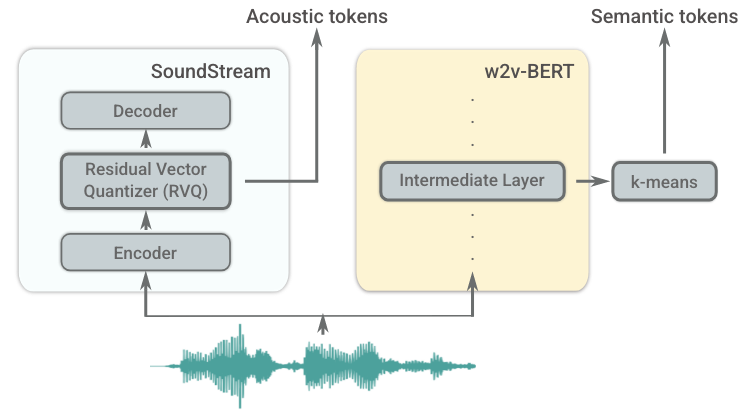
\includegraphics[width=0.5\textwidth]{tokenizerAudioLM.png}
  \caption[AudioLM Tokenisierungsverfahren]{Benutzte Tokenizer}
  \label{fig:tokenizerAudioLM}
\end{subfigure}

\vspace{1em} % Optional: Add some vertical space between the subfigures

\begin{subfigure}{1.0\textwidth}
  \centering
  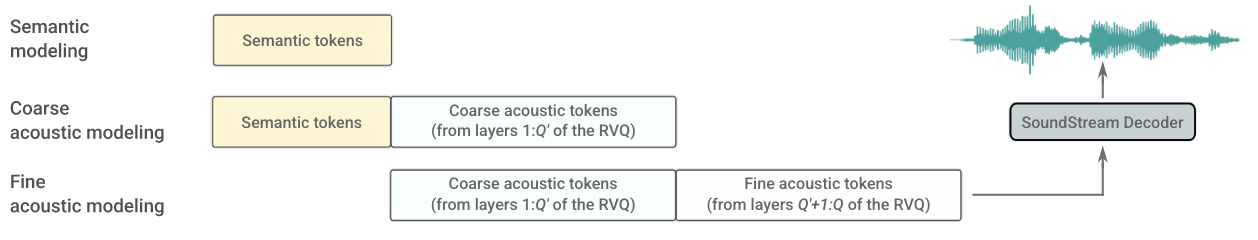
\includegraphics[width=0.7\textwidth]{hierarAudioLM.png}
  \caption[AudioLM Hierarchische Modellierung der Tokens]{Hierarchische Modellierung der Tokens}
  \label{fig:hierarAudioLM}
\end{subfigure}
\caption{AudioLM Strukturen \cite{borsos_audiolm_2022}}
\label{fig:test}
\end{figure}

\emph{Diffsound} \cite{yang_diffsound_2023} begründet seine Entwicklung mit dem Bestreben, \emph{Soundeffekte} zu generieren. Ein Audiosignal wird ebenso durch einen \emph{Prompt}, unter Verwendung eines \emph{Text Encoders}, eines \emph{Vector Quantized Variational Autoencoders (VQ-VAE)}, eines \emph{Token Decoders} sowie eines \emph{Vocoders} erzeugt (Abbildung \ref{fig:DiffsoundArchitecture}). Aus der Texteingabe extrahiert der \emph{Text Encoder} Audioinformationen und lässt unwichtige Informationen weg. Hierfür werden ein vortrainiertes \emph{BERT}\cite{devlin_bert_2019} sowie der \emph{Text Encoder} eines vortrainierten \emph{Contrastive Language-Image Pre-Training (CLIP)}\cite{radford_learning_2021} verwendet. Aus den Token wird eine Repräsentation des zu erzeugenden Audiosignals in Form eines \emph{Mel-Spektrogramms} erstellt. Da Mel-Spektrogramme als Sequenz von Tokens approximiert werden können, generiert der \emph{Token Decoder} diese aus den erzeugten Token des \emph{Text Encoders}. Die Qualität des zu produzierenden Audiosignals hängt stark von dem \emph{Token Decoder} ab. Vorherige Arbeiten wie \cite{liu_conditional_2021}, \cite{iashin_taming_2021} verwendeten hierbei einen \emph{autoregressiven} Ansatz, bei dem die folgenden Token basierend auf den vorherigen vorhergesagt werden. Dabei kann jedoch ein signifikanter akkumulierter Fehler entstehen, welcher die Performancezeit und Qualität beeinträchtigt. Um diese Schwäche zu überwinden, führt das Paper einen \emph{nicht autoregressiven Token Decoder} basierend auf \emph{Diskreter Diffusion}\cite{sohl-dickstein_deep_2015, austin_structured_2023} ein. Im Gegensatz zu dem \emph{autoregressiven} Ansatz, bei dem die Mel-Spektrogramm-Token nacheinander in Reihenfolge vorhergesagt werden, prognostiziert das Diffsound-Modell alle Mel-Spektrogramm-Token gleichzeitig und verbessert diese durch Iteration. Der \emph{VQ-VAE}\cite{oord_neural_2018} erlernt durch einen \emph{Discriminator} das Vokabular der Spektrogramm-Tokens zur Beschreibung der akustischen Ereignisse, um daraus ein Spektrogramm zu erstellen (Abbildung \ref{fig:VQVAE}). Das erzeugte Spektrogramm wird im letzten Schritt durch den \emph{Vocoder} in ein Audiosignal umgewandelt. Hierfür wurde der \emph{Vocoder} \emph{MelGAN} \cite{kumar_melgan_2019} mit dem \emph{AudioSet}\cite{gemmeke_audio_2017} Datensatz trainiert. Des Weiteren wird auch der Datensatz \emph{AudioCaps}\cite{kim_audiocaps_2019} für Training und Validierung genutzt. Diese Arbeit weist noch einige Einschränkungen auf, wie zum Beispiel, dass das Generierungsframework nicht End-to-End ist, und das Trainieren des VQ-VAE, des Token-Decoders sowie des Vocoders separat stattfindet. \cite{yang_diffsound_2023}

\begin{figure}[h]
\centering
\begin{subfigure}{1.0\textwidth}
  \centering
  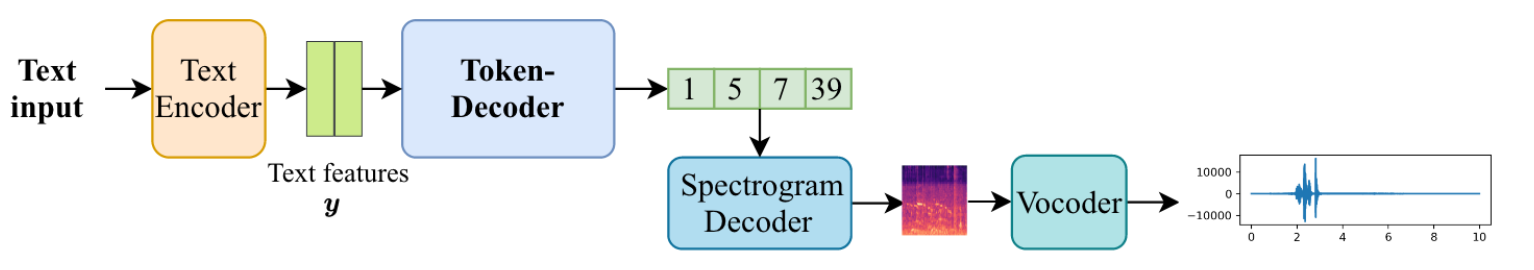
\includegraphics[width=1\textwidth]{Diffsound1.png}
  \caption[Diffsound Architektur]{Diffsound Architektur}
  \label{fig:DiffsoundArchitecture}
\end{subfigure}

\vspace{1em} % Optional: Add some vertical space between the subfigures

\begin{subfigure}{1.0\textwidth}
  \centering
  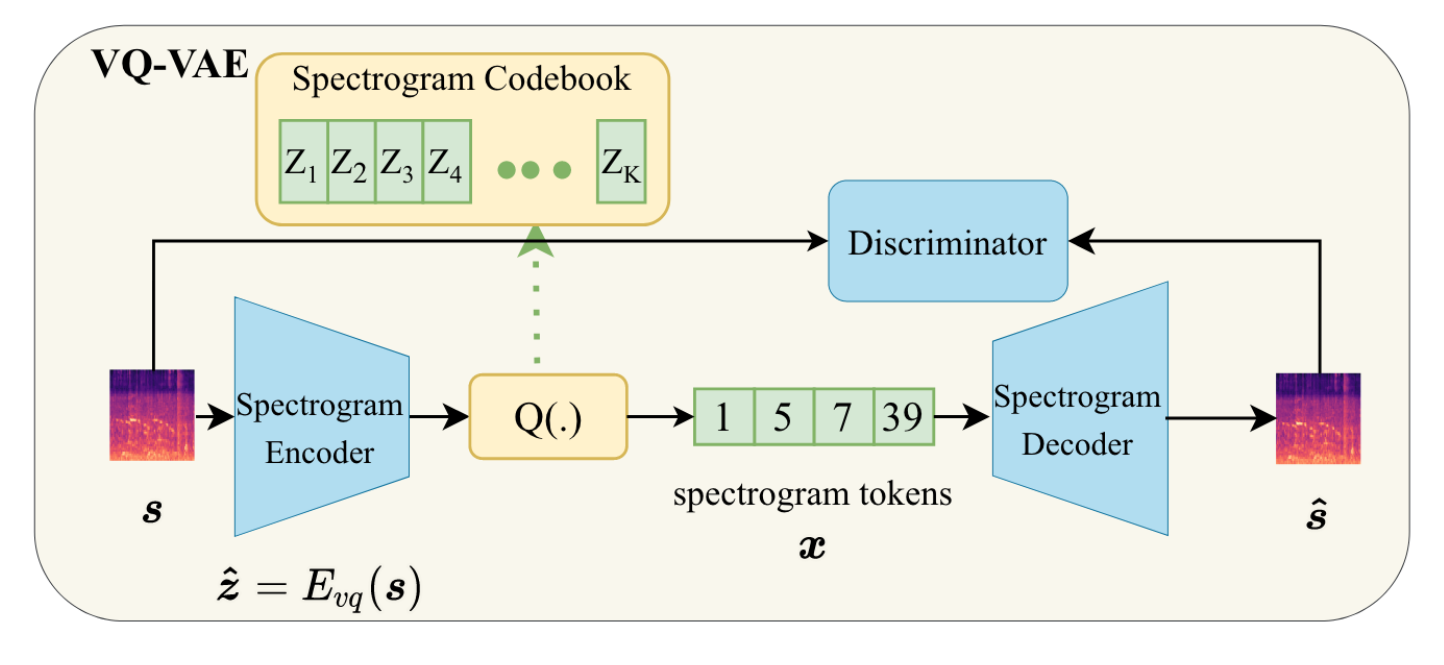
\includegraphics[width=0.7\textwidth]{Diffsound2.png}
  \caption[Diffsound VQ-VAE]{Diffsound Vector Quantized Variational Autoencoder}
  \label{fig:VQVAE}
\end{subfigure}
\caption{Diffsound Strukturen \cite{yang_diffsound_2023}}
\label{fig:test}
\end{figure}

\emph{Tango} \cite{ghosal_text--audio_2023} basiert auf der Struktur und den Konzepten von \emph{AudioLDM}, mit dem Ziel, Text zu Audio mittels latenter Diffusion umzuwandeln. Dabei unterscheidet es sich in wesentlichen Punkten von \emph{AudioLDM} und verspricht, bessere Ergebnisse mit einem reduzierten Datensatz zu erzielen. Die Architektur besteht aus drei Hauptkomponenten (Abbildung \ref{fig:tango}): einem \emph{Text Encoder} für die einzugebenden Prompts, einem \emph{Latenten Diffusionsmodell} (\emph{LDM})\cite{rombach_high-resolution_2022} und einem \emph{Variational Autoencoder} (\emph{VAE})\cite{kingma_auto-encoding_2022}. Der \emph{Text Encoder} generiert unter Verwendung des \emph{Large Language Model} (\emph{LLM}) \emph{FLAN-T5-LARGE} \cite{chung_scaling_2022} eine textuelle Repräsentation der Eingabe. Wie durch \cite{dai_why_2023} belegt, sind \emph{FLAN-T5-Modelle} dazu in der Lage, neue Aufgaben effizient und zügig zu erlernen, da sie über eine umfangreiche Datenmenge an Gedankengängen, Argumentationsketten und Instruktionen vortrainiert wurden. Dieses umfangreiche Vortraining, das bei früheren Text-Modellen wie \emph{RoBERTa}\cite{liu_roberta_2019}, die für die Audiosynthese verwendet wurden, fehlt, könnte dem Encoder die Hervorhebung von Schlüsseldetails erleichtern. Dies könnte wiederum zu einer verbesserten Umwandlung von Umschreibungen in akustische Entsprechungen führen. Das \emph{LDM}, übernommen von \emph{AudioLDM}, erzeugt aus der textuellen Repräsentation des Prompts eine latente Audio-Repräsentation in Form von Spektogramm-Tokens. Dieser Prozess wird durch das koordinierte Zusammenspiel des Vorwärts- und Rückwärtsdiffusionsprozesses erlernt, wobei der Audio-Repräsentation Rauschen hinzugefügt und diese dann unter Textführung wieder entrauscht wird. Während der Inferenz wird der erlernte Rückwärtsdiffusionsprozess verwendet, um die Audio-Repräsentation zu erzeugen. Anschließend generiert der Decoder des \emph{VAE} daraus ein Mel-Spektogramm. Der gleiche  \emph{Vocoder} \emph{HiFi-GAN}\cite{kong_hifi-gan_2020}, der auch bei \emph{AudioLDM} verwendet wurde, dient dazu, aus dem Spektogramm ein Audiosignal zu erzeugen. Das Modell stößt auf Limitierungen bei der Generierung differenzierter Audioausgaben für ähnliche Textaufforderungen, wenn es lediglich auf einem kleinen Datensatz trainiert wurde. Die Autoren schlagen daher vor, diese Limitierung zu überwinden, indem das Modell in Zukunft auf größeren Datensätzen trainiert wird, um seine Fähigkeiten zur Differenzierung und Generierung verschiedener Text-Audio-Zuordnungen zu verbessern.

\begin{figure}[h]
  \centering
  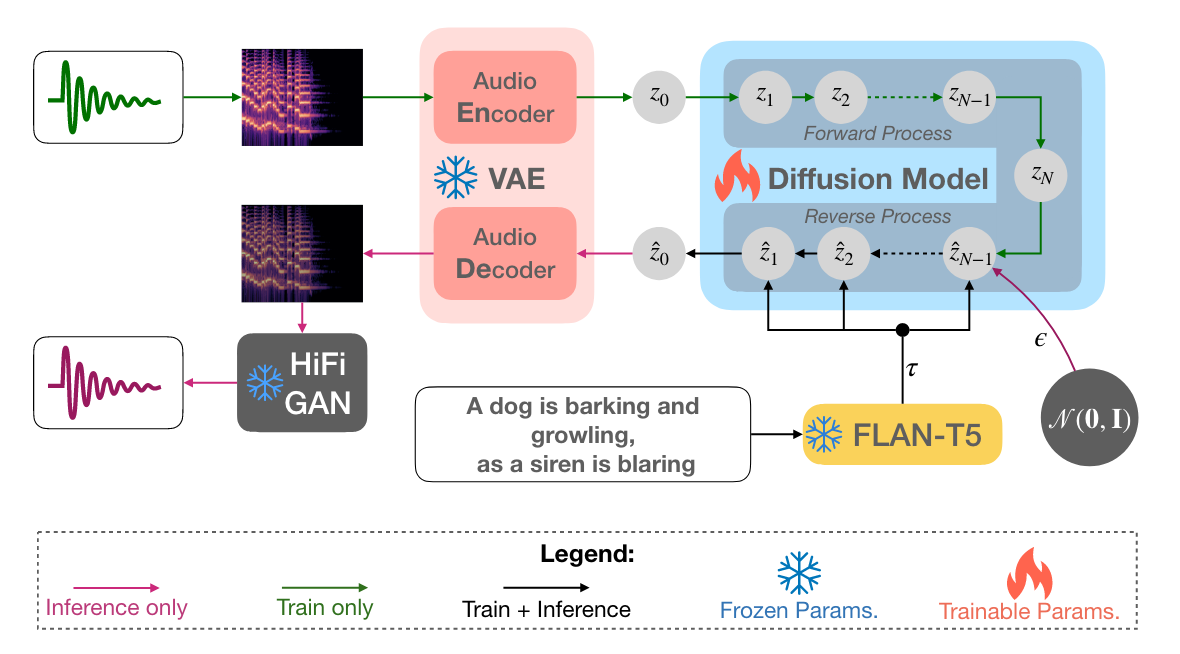
\includegraphics[width=.7\textwidth]{graphics/Tango.png}
  \caption[Tango Architektur]{Tangos Architektur \cite{liu_roberta_2019}}
  \label{fig:tango}
\end{figure}

TODO: AudioLDM2 

\emph{AudioGen} \cite{kreuk_audiogen_2023}, \emph{Make-An-Audio} \cite{huang_make--audio_2023}.


Die musikalische Anwendung von \emph{Artifical Intelligence} beschränkt sich nicht nur auf die textbasierte Synthesisierung von Klängen.







\chapter{Methoden}

\section{Klangsynthese und Musikproduktion}

\subsection{Mathematische und physikalische Modellierung von Musik und Klang}\label{sec:music_math}
\glqq Musik ist eine Kunstform und kulturelle Aktivität, deren Medium der in Zeit organisierte Klang ist\grqq \footnote{"Music is an art form and cultural activity whose medium is sound organized in time"} \cite{tsuji_physics_2021}. Im Gegensatz zu Rauschen weisen die Klänge, die Musik aufbauen, Strukturen und Zusammenhänge auf, welche für das menschliche Gehör als angenehm wahrgenommen werden \cite{parker_good_2009}. 

\emph{Klang} stellt ein intrinsisches Zusammenspiel aus physikalischen und perzeptiven Elementen dar. Auf physikalischer Ebene handelt es sich bei Klang um eine durch einen schwingenden Körper erzeugte Welle, die sich von einem Ort zum anderen propagiert. Diese Welle besteht aus einem Grundton und mehreren resonierenden Einzeltönen. Der resultierende Klang besitzt eine Vielzahl von Obertönen, die die charakteristischen klanglichen Eigenschaften oder \emph{Klangfarben} hervorbringen. \cite{tsuji_physics_2021, parker_good_2009}

Diese verschiedenen \emph{Töne} sind periodische Schwingungen, definiert durch eine \emph{Tonhöhe/Frequenz} $\omega$ (in $Hz$), welche als die Anzahl der Kompressionen an einem bestimmten Punkt pro Sekunde interpretiert werden kann. Der Kehrwert der Frequenz wird als \emph{Periode} $T=\frac{1}{\omega}$ (in $s$) bezeichnet und beschreibt die Zeit, die eine Kompression benötigt, um zwei identische Punkte zu passieren. Unsere Wahrnehmung lässt Töne mit niedriger Frequenz tief und dumpf klingen, während hohe Frequenzen als leicht, schwebend und durchdringend wahrgenommen werden. Die \emph{Amplitude} der Schwingung beschreibt die transportierte Energie und somit die Lautstärke eines Tones. Aufgrund des Abstandsgesetzes wird diese von einer Schallquelle über die logarithmische \emph{Dezibel-Skala} (dB) angegeben.  \cite{tsuji_physics_2021, parker_good_2009}

Die Untersuchung der Struktur eines Klangs befasst sich mit den Relationen und Zusammenhängen der verschiedenen Töne, aus denen der Klang besteht. Die einfachste Form eines Tones ist der Sinuston, dessen Schwingung durch eine Sinuskurve dargestellt wird. Gemäß dem Fouriertheorem setzt sich jeder andere Ton aus verschiedenen Sinustönen zusammen (Abbildung \ref{fig:evolution}), wobei die tiefste dominante Frequenz als \emph{Grundton} und die höheren Frequenzen als \emph{Obertöne} bezeichnet werden. Die Obertöne unterscheiden sich in Frequenz, Amplitude und zeitlichem Auf- und Abbau. Wenn die Frequenz eines Obertones ein ganzzahliges Vielfaches des Grundtones ist, wird dieser als \emph{harmonischer} Oberton bezeichnet. Im Falle, dass der Oberton kein ganzzahliges Vielfaches des Grundtones ist, spricht man von einem \emph{inharmonischen} Oberton. Daher erzeugen unterschiedliche Instrumente, die die gleiche Note spielen, die gleiche Grundschwingung, weisen jedoch unterschiedliche harmonische und inharmonische Obertöne auf. \cite{parker_good_2009, white_physics_2014, ruschkowski_elektronische_2019}

\begin{figure}
  \centering
  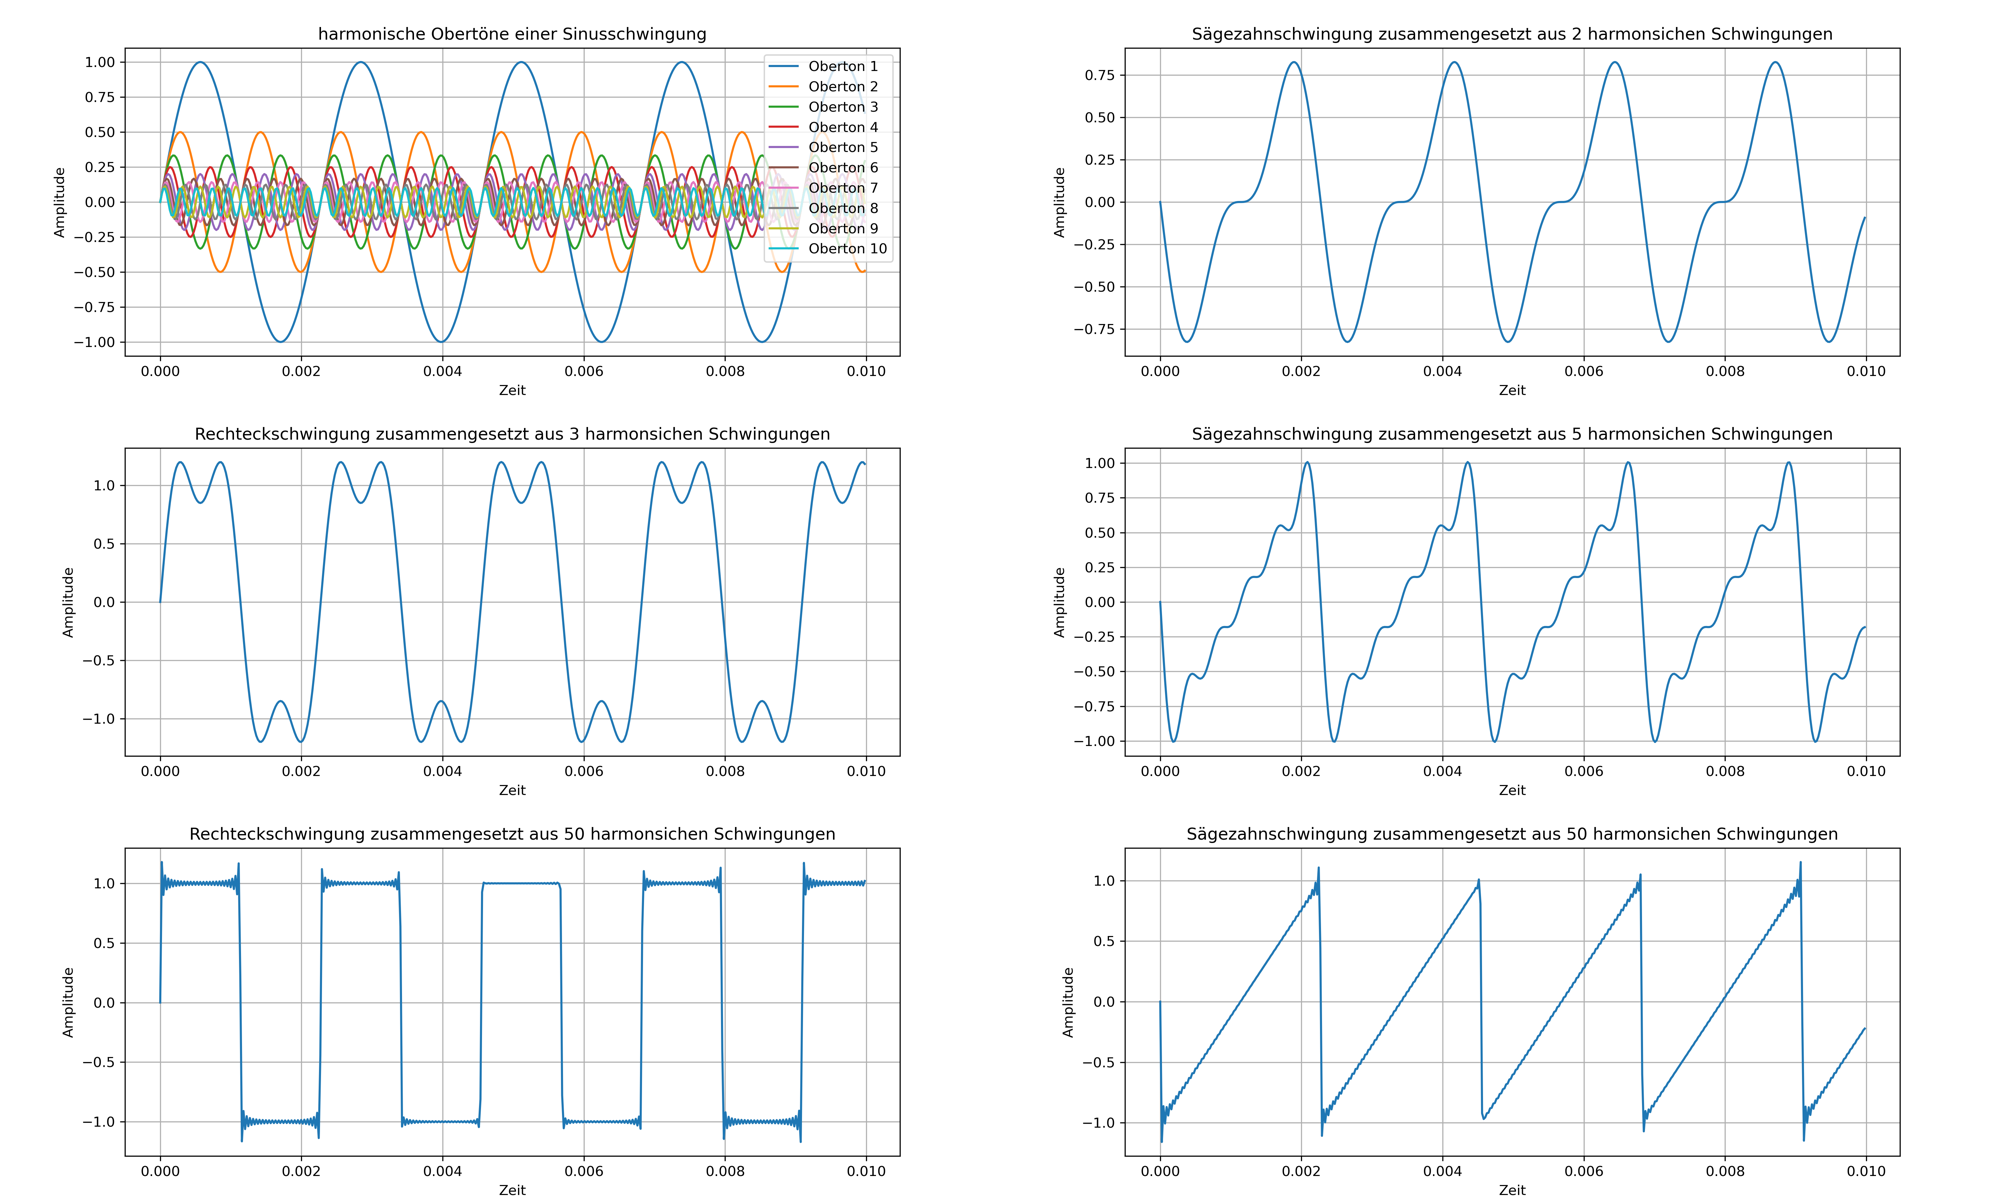
\includegraphics[width=1.0\textwidth]{evolution.png}
  \caption[Fourier Reihe]{Zusammensetzung Sägezahn- und Rechtecksschwingungen aus harmonischen Oberschwingungen einer Sinusschwingung}
  \label{fig:evolution}
\end{figure}

Die Struktur eines Klangs kann durch die Amplitudenfaktoren und zugehörigen Frequenzen der einzelnen Töne beschrieben und in einem \emph{Frequenzspektrum} (Abbildung \ref{fig:spectro}) visualisiert werden. Dies erlaubt die Bestimmung, welche Frequenzen oder Frequenzbereiche im Signal besonders stark enthalten sind und ermöglicht eine Darstellung der Klangfarbe bzw. der Charakteristik. Mit einer \emph{Fourier-Transformation} kann für jedes beliebige Signal das entsprechende Spektrum ermittelt und durch die \emph{Inverse Fourier-Transformation} das Signal eines Spektrums berechnet werden. \cite{raffaseder_audiodesign_2010}

Zur Berechnung einer \emph{Diskreten Fourier-Transformation (DFT)} hat sich die \emph{Fast Fourier-Transformation (FFT)} als effizienter Algorithmus etabliert \cite{heideman_gauss_1985}. Um die Foruier-Transformation in Echtzeit durchzuführen wird die \emph{Short Time Fourier-Transformation} angewandt \cite{thyagarajan_introduction_2019}. 

Ein \emph{Spektrogramm} ermöglicht die Betrachtung eines Signals sowohl im Zeit- als auch im Frequenzbereich (Abbildung \ref{fig:spectro}), allerdings nicht in beliebiger Genauigkeit. Da hier das Signal in kurze zeitliche Abschnitte unterteilt und für diese das Spektrum berechnet wird, verlieren längere Abschnitte Informationen über die zeitliche Auflösung, weisen jedoch eine bessere Frequenzauflösung auf. Kurze Abschnitte hingegen besitzen eine bessere zeitliche Auflösung, lösen jedoch weniger genau im Frequenzbereich auf. \cite{raffaseder_audiodesign_2010}

Ein Klang wird als \emph{Rauschen} bezeichnet, wenn er ein kontinuierliches Frequenzspektrum aufweist, das viele Arten von Geräuschen aus unterschiedlichen Quellen umfasst
\cite{tsuji_physics_2021}. 

Der durch das menschliche Gehör erfassbare Frequenzbereich ($20 Hz$ -  $20kHz$) wird in drei Bereiche (\emph{Bässe, Mitten, Höhen}) unterteilt. Bässe sind in einem Bereich von $20Hz$ bis $250Hz$ auffindbar, während tiefe Mitten den Bereich von 250$Hz$ bis $2000Hz$ umschließen. Hohen Mitten erstrecken sich von $2kHZ$ bis $4kHz$. Die Höhen liegen oberhalb von $4kHz$. \cite{raffaseder_audiodesign_2010}

\begin{figure}
  \centering
  \includegraphics[width=1.0\textwidth]{spectrums_flat.png}
  \caption[Fourier Reihe]{Spektren, Spektrogramme und Mel-Spektrogramme verschiedener Klänge}
  \label{fig:spectro}
\end{figure}


\subsection{Digitale Audiorepräsentation und Sampling}. 

Bedingt durch die binäre Natur digitaler Computer ist für die Repräsentation und Verarbeitung von Audiosignalen eine Transformation des Signals von einem kontinuierlichen zu einem diskreten Wertebereich erforderlich. Das \emph{Abtasttheorem} besagt, dass analoge Signale überflüssige Informationen enthalten, die bei einer Übertragung weggelassen werden können. Es reicht somit aus, das Audiosignal zu reproduzieren, indem Amplitudenwerte in regelmäßigen Zeitabständen entnommen und übertragen werden. Um das Signal vollständig beschreiben zu können, muss die Abtastrate mindestens das Zweifache der höchsten Frequenz des Signals betragen. Dieser Grenzwert wird als \emph{Nyquist-Frequenz} definiert und entspricht $2 \omega \mathrm{Hz}$. Da das menschliche Gehör nur Frequenzen bis zu $20kHz$ wahrnimmt, wird in der Praxis häufig eine \emph{Abtastrate} von $44.1kHz$ verwendet. Fällt die Abtastrate unter die Nyquist-Frequenz, gehen Informationen verloren und die wiederhergestellte Wellenform kann von der originalen Form abweichen. In einem solchen Fall ist der Prozess der Signalerneuerung nicht mehr deterministisch, was als \emph{Unterabtastung} bezeichnet wird. \cite{lai_practical_2004, shannon_communication_1949, ruschkowski_elektronische_2019}

Die \emph{Samplingtiefe (engl. Bitdepth)} gibt den Wertebereich an, in dem die ausgelesenen Amplitudenwerte abgebildet werden. Je größer dieser ist, desto treuer kann das original Signal repräsentiert werden, jedoch wird hierfür auch mehr Speicher benötigt. Fällt der Wertebereich klein aus, so müssen die Amplitudenwerte stärker gerundet werden und daher Artefakte und Fehler im Signal entstehen. \cite{thompson_understanding_2005}

\emph{Sound-Sampling} oder \emph{Sampling} als Kombination mit digitaler/analoger Klangmanipulation ist eine eigenständige Klangsynthesetechnik, obwohl es im Kern nur eine Wiedergabe des entnommen Signals ist, und somit nicht nur eine einfache Speicherung. Die Prinzipen und Methoden aus der analogen Synthetisierung und Klangformung können auf die Wiedergabe des Klanges angewandt werden. Das entstandene Instrument wird als \emph{Sampler} bezeichnet. Je nach Komplexität des Instruments erlaubt es den Spieler, das Signal in einem gewünschten Bereich zu wiederholen, es zu verlangsamen, verschnellern, umzudrehen, oder bestimmte Intervalle neu zu arrangieren. Dadurch eröffnet sich ebenfalls die Möglichkeit des musikalischen Zitierens und damit auch das Problem des klanglichen Diebstahls für Musiker, Verlage und Plattenfirmen. \cite{russ_sound_2009, ruschkowski_elektronische_2019, katz_capturing_2010} 

Die Wiederverwendung und Aufarbeitung von Ausschnitten oder kompletten schon produzierten Werken ist in der Industrie Gang und Gebe und etwas was mit Hilfe von generativer Küntslichen Intelligenz vermieden werden kann. 

\subsection{Synthetisierung und Klangformung} \label{sec:synth+envelope}

Instrumente, die zur Generierung und Manipulation von musikalischen Klängen durch elektronische Spannung dienen, werden als Synthesizer bezeichnet \cite{dudenredaktion_synthesizer_nodate, pirkle_designing_2021}. Die Komponenten eines solchen Instruments können in drei Kategorien unterteilt werden (Abbildung \ref{fig:synth}): \emph{Erzeuger} (eng. \emph{source}), \emph{Modifikatoren} und \emph{Kontrollinstanzen}. Erzeuger wie Oszillatoren generieren den ursprünglichen Klang, der in diesem spezifischen Projekt mittels Diffusion erzeugt wird. Modifikatoren, darunter Filter und Effekte, manipulieren diesen erzeugten Klang. Kontrollinstanzen bieten dem Anwender die Möglichkeit, die Parameter der Erzeuger und Modifikatoren einzustellen und dynamisch anzupassen. Das Manipulieren eines Parameters wird als \emph{Modulieren} bezeichnet. Die Spezifischen Einstellungen der Parameters als \emph{Patch}. \cite{pirkle_designing_2021}   

Die für das Umsetzen des Projektes benötigten Komponenten werden im Folgenden erklärt. 

\begin{figure}[h]
  \centering
  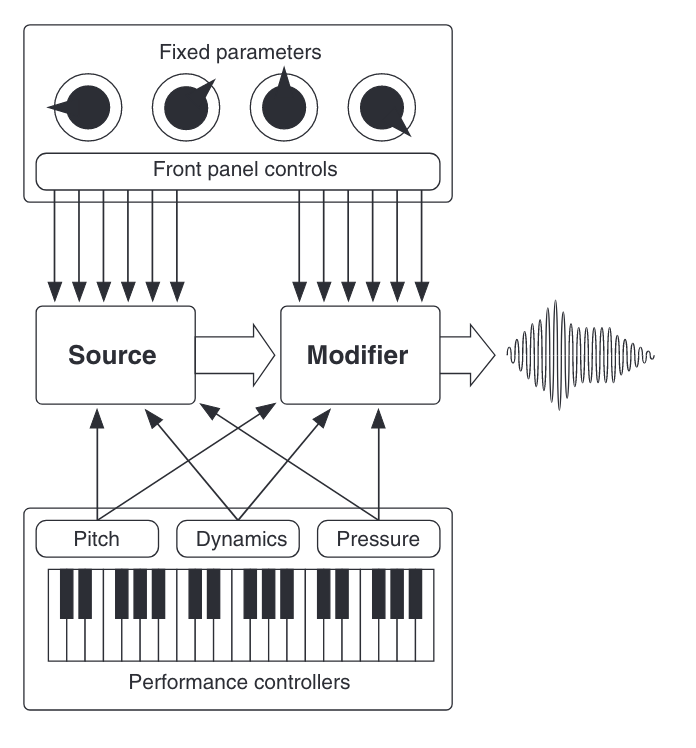
\includegraphics[width=.5\textwidth]{graphics/synthstruc.png}
  \caption[Synth]{Komponenten eines Synthesizers \cite{russ_sound_2009}}
  \label{fig:synth}
\end{figure}

In dem Bestreben, sein erworbenes wissenschaftliches Verständnis und seine Expertise in die Konstruktion musikalischer Instrumente einzubringen, entwickelte der Physiker und Komponist Hugh Le Caine erste Geräte zur elektronischen Klangsynthese, 20 Jahre vor der Kommerzialisierung der ersten analogen Synthesizer \cite{young_gale_hugh_2013}. Le Caine formuliert in diesem Kontext eine Reihe von Prinzipien, die ein Instrumentenbauer seiner Ansicht nach anstreben sollte. Er vertrat die Überzeugung, dass ein Spieler die maximale Kontrolle über die wichtigsten Parameter eines Klangs besitzen sollte. Er erkannte, dass sich die Expressivität eines Instruments insbesondere durch die Kontrolle der \emph{Anschlagsdynamik} über den gesamten Lautstärkebereich eines Tones, durch die Kontrolle seiner \emph{An- und Ausschwingszeiten} sowie der Klangfarbe definiert. \cite{ruschkowski_elektronische_2019}

\begin{figure}[h]
  \centering
  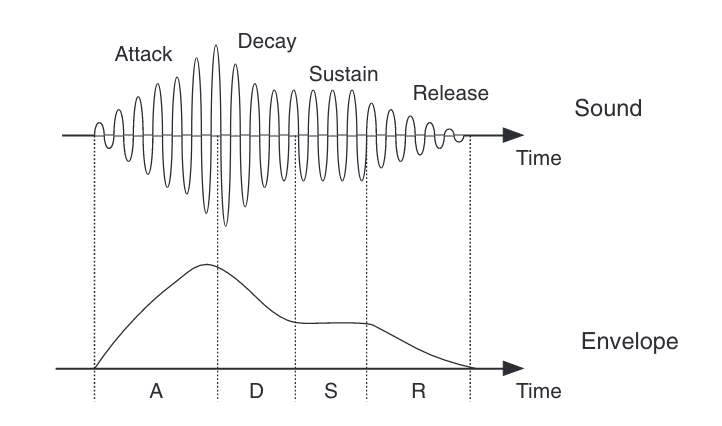
\includegraphics[width=.7\textwidth]{graphics/ADSR.png}
  \caption[ADSR]{Beispiel einer Hüllkurve \cite{russ_sound_2009}}
  \label{fig:adsr}
\end{figure}

Generell wird danach gestrebt, Klänge zu erzeugen, die sich sowohl in der Zeit als auch in der Frequenz entwickeln, verändern oder morphieren, um klanglich interessante Ereignisse zu schaffen \cite{pirkle_designing_2021}. Die Kontrolle über Anschlagsdynamik sowie An- und Ausschwingszeiten wird mittels eines Hüllkurvengenerators (engl. envelope generator) erreicht. Ein solcher Generator setzt sich typischerweise aus vier Komponenten zusammen. Die Anschwellzeit (engl. attack time) definiert das Intervall, welches nach Betätigen einer Taste verstreicht, bis ein Ton seine maximale Lautstärke erreicht. Analog dazu kennzeichnet die Abschwellzeit (engl. decay time) den Zeitraum, in dem der Ton bis zu einem vorab festgelegten Lautstärkelevel (engl. sustain level) absinkt. Dieses Level wird solange aufrechterhalten, bis die Taste wieder freigegeben wird. Nach dieser Freigabe kann ein weiteres Zeitintervall festgelegt werden, in dem der Ton vollständig ausklingt (engl. release time). Aufgrund der Nomenklatur dieser Komponenten wird der Generator häufig als ADSR-Generator(engl. \emph{attack, decay sustain, release}) (Abbidlung \ref{fig:adsr})  bezeichnet. Instrumente, wie beispielsweise mit einem Bogen gespielte Streichinstrumente, weisen lange Anschlag-, Abschwell- und Ausschwingzeiten haben. Im Gegensatz dazu haben Zupfinstrumente kürzere Angriffszeiten. Klaviere und Schlaginstrumente haben sehr schnelle Angriffszeiten. \cite{ruschkowski_elektronische_2019, russ_sound_2009}

Die durch den spezifischen Erzeuger entstandene Klangfarbe, kann mittels Filtern weiterhin modifiziert werden. In der Elektrotechnik dienen diese dazu, bestimmte Frequenzbereiche zu eliminieren. Dabei spielen vor allem der sogenannte \emph{Tiefpassfilter} (engl. \emph{low-pass}) und \emph{Hochpassfilter} (engl. \emph{high-pass}) eine zentrale Rolle, welche jeweils die höheren oder tieferen Bereiche des Spektrums unterdrücken. Der Grenzwert, an dem diese Unterdrückung initiiert wird, ist als \emph{Beschneidungsfrequenz} (engl. \emph{cut-off-frequency}) bekannt. Mithilfe der genannten Filter besteht die Möglichkeit, gewünschte oder ungewünschte Obertöne zu dämpfen oder zu isolieren. Eine sequenzielle Anordnung dieser Filter resultiert in einem \emph{Bandpassfilter}. Oftmals bietet sich zudem die Gelegenheit, Obertöne im Bereich der Beschneidungsfrequenz zu intensivieren, wodurch eine \emph{Resonanz} (engl. \emph{resonance}) simuliert wird. \cite{ruschkowski_elektronische_2019}

Kontrollinstanzen lassen sich in zwei Kategorien untergliedern. Die erste Kategorie umfasst Performance-gesteuerte Steuerungselemente, wie beispielsweise ein Klaviaturkeyboard, welches dem Musiker ermöglicht, die Tonhöhe nach seinen individuellen Präferenzen anzupassen und somit das Instrument zu manipulieren sowie zu beherrschen. Die zweite Kategorie besteht aus festen, synthesizerspezifischen Parametern, die dazu dienen, den Charakter des gewünschten Klangs einzustellen und zu formen. Hierzu zählen beispielsweise die Regler und Knöpfe eines Synthesizers. \cite{russ_sound_2009}

Für die Vereinheitlichung der Parametersteuerung und Kommunikation zwischen elektronischen Geräten wurde das Kommunikationsprotokoll MIDI (Musical Instrument Digital Interface)\cite{midi_association_midi_nodate} entwickelt . Dieses hat sich als internationaler Standard in der Welt der elektronischen Musik durchgesetzt und ermöglicht es MIDI-Instrumenten, Informationen zu empfangen und zu senden. \cite{ruschkowski_elektronische_2019}

Die Einführung dieses Protokolls beeinflusste signifikant die Konzeption und Gestaltung von Synthesizern. Durch die Einheitlichkeit vieler Aspekte des Synthesizer-Designs, bedingt durch das MIDI-Protokoll, rückte die Methode der Klangerzeugung stärker in den Vordergrund, während das funktionale Design des Instruments in den Hintergrund trat. \cite{russ_sound_2009}

\section{Synthetisierung mittels Diffusion}

\glqq Die Methoden der Klangerzeugung mit traditionellen mechanischen Musikinstrumenten waren seit ihrer Entstehung nur unwesentlichen Veränderungen unterworfen. [...] Der Instrumentenbau wandelte sich lediglich deshalb im Laufe der Zeit, weil man die Spielbarkeit der Instrumente zu verbessern und ihren Klangcharakter den wechselnden musikalischen Idealvorstellungen anzupassen wünschte. Anders dagegen im Bereich elektronischer Klangerzeugung. Hier werden ständig neue Methoden zur Synthese von Klängen entwickelt.\grqq \, \cite{ruschkowski_elektronische_2019}

Im Folgenden soll zunächst dargelegt werden, welche Vorteile die neuartige Technik der Soundsynthese durch Diffusion mit sich bringen kann. Bei Erzielung von hochwertigen Ergebnissen könnten beispielsweise die Notwendigkeit und der Zugang zu aufgezeichneten Klängen entfallen. Der Aufwand für die Aufnahme solcher Klänge ist oft erheblich und führt daher in der Regel zu kostenpflichtigen Angeboten. Die Anwendung künstlicher Intelligenz in der Synthese von Sound könnte jedoch dazu beitragen, diesen Bereich zu demokratisieren und einem breiteren Publikum die benötigten Ressourcen zur Verfügung zu stellen. Darüber hinaus könnte diese Technik den Nutzern eine umfassendere Kontrolle über die gewünschten Eigenschaften und Klangfarben verleihen. Auf kreativer Ebene ermöglicht die Soundsynthese durch Diffusion die Erzeugung einzigartiger, zuvor nicht existierender Klänge, die potenziell als neue Inspirationsquelle für Künstler und Musiker dienen könnten. \cite{haohe_liu_audioldm_2023-1}


\subsection{Diffusion}
Unter der Prämisse, dass die untersuchten Daten einer bestimmten Verteilung entstammen, verfolgen generative Machine-Learning-Modelle das Hauptziel, diese Verteilung zu identifizieren und zu approximieren. Die Generierung neuer Daten basiert auf der Entnahme einer Probe aus der approximierten Verteilung.\cite{machine_learning_at_berkeley_diffusion_2022}

Der im Kontext des Maschinellen Lernens als \emph{Diffusion} bekannte Prozess\cite{sohl-dickstein_deep_2015, ho_denoising_2020, nichol_improved_2021, dhariwal_diffusion_2021} schöpfte seine Inspiration aus der statistischen Thermodynamik\cite{jarzynski_equilibrium_1997} und der sequenziellen Monte-Carlo-Methodik\cite{neal_annealed_1998}. Hierbei zielt man darauf ab, iterative korrumpierte Strukturen einer Datenverteilung $x_0\sim q(\mathbf{x}_0)$ (\emph{forward diffusion}) durch einen Rückwärtsprozess zu korrigieren (\emph{reverse diffusion}). Dies resultiert in einem generativen Modell, welches effizient trainiert und bewertet werden kann als vergleichbare Methoden.\cite{sohl-dickstein_deep_2015, nichol_improved_2021}

\begin{figure}[h]
  \centering
  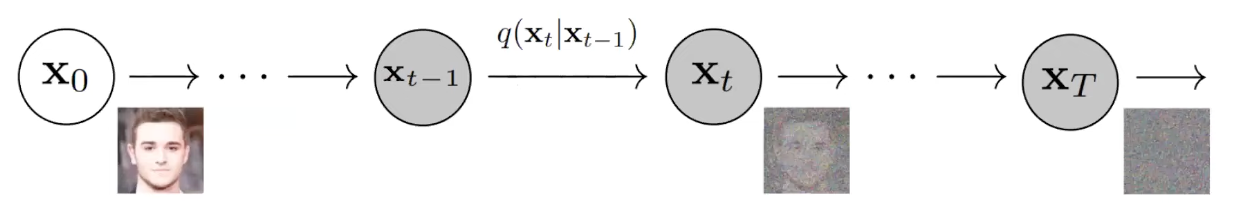
\includegraphics[width=.9\textwidth]{forwardDiffusion.png}
  \caption[Forward diffusion]{Vorwärtsprozess Diffusion \cite{machine_learning_at_berkeley_diffusion_2022}}
  \label{fig:forwardDiffusion}
\end{figure} 

Der Vorwärtsprozess (Abbildung \ref{fig:forwardDiffusion}) wurde als Markov-Kette konzipiert\cite{sohl-dickstein_deep_2015, ho_denoising_2020}. Einem Datenpunkt $x_0$ wird eine minimale Menge an Rauschen hinzugefügt, welches durch den Hyperparameter $\left\{\beta_t \in(0,1)\right\}_{t=1}^T$, als \emph{noise schedule} bekannt, definiert wird\cite{ho_denoising_2020, machine_learning_at_berkeley_diffusion_2022}. Dabei wird \emph{Gauss'sches Rauschen}\cite{shannon_communication_1949} verwendet, welches durch eine Normalverteilung $\mathcal{N}$ beschrieben wird. Wird dieser Prozess über $T$-Schritte wiederholt, verliert man nach und nach Informationen, bis letztlich nur isotropisches Rauschen zurückbleibt\cite{machine_learning_at_berkeley_diffusion_2022}.

\begin{align}
   & q\left(\mathbf{x}^{(t)} \mid \mathbf{x}^{(t-1)}\right) = \mathcal{N}\left(\mathbf{x}^{(t)} ; \mathbf{x}^{(t-1)} \sqrt{1-\beta_t}, \mathbf{I} \beta_t\right) \\
   & q\left(\mathbf{x}_{1: T} \mid \mathbf{x}_0\right)=\prod_{t=1}^T q\left(\mathbf{x}_t \mid \mathbf{x}_{t-1}\right)
\end{align}

Mit den Beziehungen \( \alpha_t:=1-\beta_t \) und \( \bar{\alpha}_t:=\prod_{s=1}^t \alpha_s \) ergibt sich für den Vorwärtsprozess die Gleichung:

\begin{equation}
    q\left(\mathbf{x}_t \mid \mathbf{x}_0\right)=\mathcal{N}\left(\mathbf{x}_t ; \sqrt{\bar{\alpha}_t} \mathbf{x}_0,\left(1-\bar{\alpha}_t\right) \mathbf{I}\right)
\end{equation}

\begin{figure}[h]
  \centering
  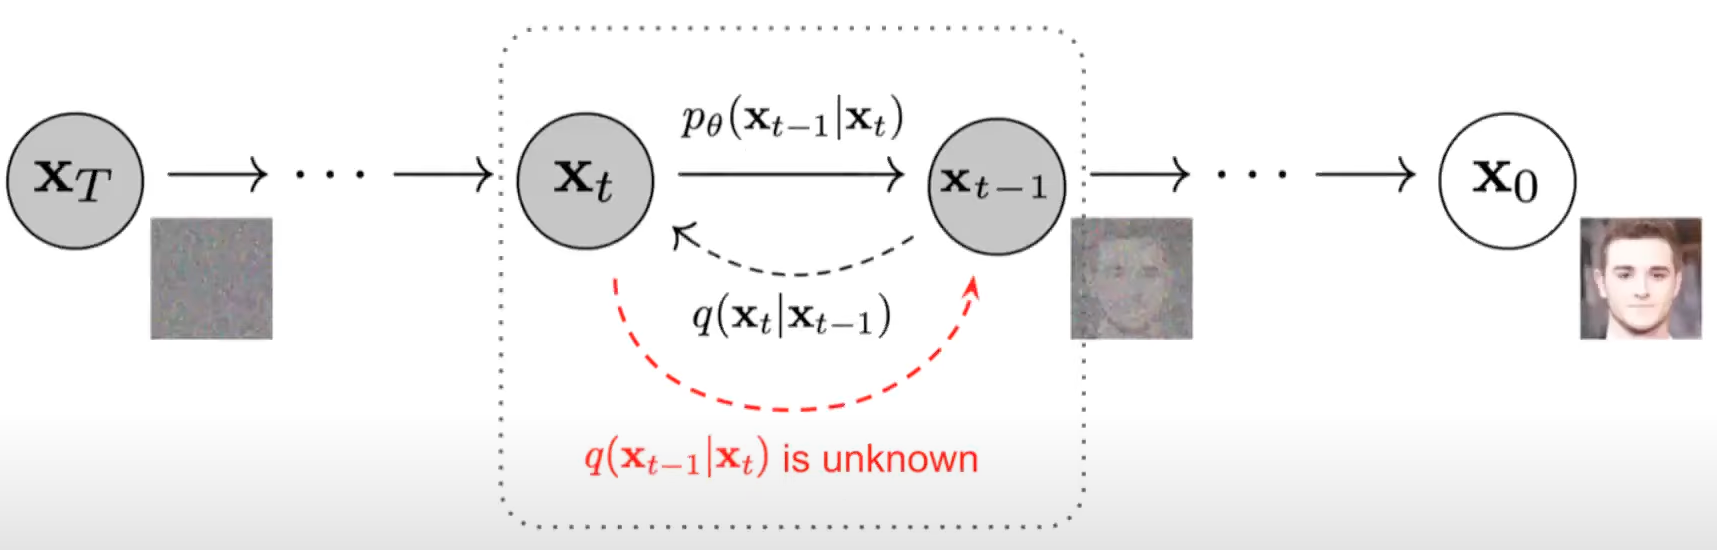
\includegraphics[width=.8\textwidth]{reverseDiffusion.png}
  \caption[Reverse diffusion]{Rückwertsprozess Diffusion \cite{machine_learning_at_berkeley_diffusion_2022}}
  \label{fig:reverseDiffusion}
\end{figure} 

Im Rückwärtsprozess (Abbildung \ref{fig:reverseDiffusion}) wird angestrebt, das hinzugefügte Rauschen $\epsilon \sim \mathcal{N}(0,1)$ iterativ zu eliminieren \cite{machine_learning_at_berkeley_diffusion_2022}. Dadurch erscheint es, als würde der inverse Prozess neue Daten aus Rauschen generieren \cite{machine_learning_at_berkeley_diffusion_2022}. Bei geringem $\beta$ entspricht die Rauschverteilung des Rückwärtsschritts \( q\left(\mathbf{x}_{t-1} \mid \mathbf{x}_t\right) \) dem Vorwärtsprozess \cite{sohl-dickstein_deep_2015}. Der erlernte Rückwärtsprozess \( p_\theta\left(\mathbf{x}_{t-1} \mid \mathbf{x}_t\right) \) kann daher wie folgt approximiert werden \cite{ho_denoising_2020, machine_learning_at_berkeley_diffusion_2022, nichol_improved_2021}. Der Lernprozess konzentriert sich darauf, geringfügige Abweichungen zu schätzen, anstatt den gesamten Prozess in einem Schritt durch eine Funktion darzustellen \cite{sohl-dickstein_deep_2015}.


\begin{align}
& p_\theta\left(\mathbf{x}_{t-1} \mid \mathbf{x}_t\right)=\mathcal{N}\left(\mathbf{x}_{t-1} ; \boldsymbol{\mu}_\theta\left(\mathbf{x}_t, t\right), \boldsymbol{\Sigma}_\theta\left(\mathbf{x}_t, t\right)\right)\\
& p_\theta\left(\mathbf{x}_{0: T}\right)=p\left(\mathbf{x}_T\right) \prod_{t=1}^T p_\theta\left(\mathbf{x}_{t-1} \mid \mathbf{x}_t\right)
\end{align}

Das Erlernen des Rückwärtsprozesses erfolgt durch ein neuronales Netzwerk, wobei in jedem Schritt der Erwartungswert $\boldsymbol{\mu}_\theta$, das ursprüngliche Bild $\boldsymbol{x}_0$ oder das eingefügte Rauschen $\boldsymbol{\epsilon}$ vorhergesagt werden können \cite{ho_denoising_2020, nichol_improved_2021}. Es wurde festgestellt, dass Bildvorhersagen schlechtere Ergebnisse erzielten und daher sich für die Vorhersage des eingefügten Rauschens $\boldsymbol{\epsilon}$ mit der vereinfachten Verlustfunktion 3.6 entschieden wurde \cite{ho_denoising_2020}.

\begin{equation}
    L_{\text {simple }}=E_{t, x_0, \epsilon}\left[\left\|\epsilon-\epsilon_\theta\left(x_t, t\right)\right\|^2\right]
\end{equation}

Aus dem vorhergesagten Rauschen $\boldsymbol{\epsilon}$ kann der Erwartungswert $\boldsymbol{\mu}_\theta$ mit folgender Gleichung hergeleitet werden:

\begin{equation}
    \mu_\theta\left(x_t, t\right)=\frac{1}{\sqrt{\alpha_t}}\left(x_t-\frac{\beta_t}{\sqrt{1-\bar{\alpha}_t}} \epsilon_\theta\left(x_t, t\right)\right)
\end{equation}

Die in \cite{ho_denoising_2020} präsentierte Architektur des neuronalen Netzwerks basiert auf einem \emph{U-Net} \cite{ronneberger_u-net_2015}, welches auf einem \emph{Wide ResNet} \cite{zagoruyko_wide_2017} aufbaut \cite{ho_denoising_2020}.

\cite{nichol_improved_2021} führte bedeutende Verbesserungen gegenüber den Arbeiten von \cite{sohl-dickstein_deep_2015} und \cite{ho_denoising_2020} ein. Anstatt mit einer festen Varianz zu trainieren, wurde diese nun ebenfalls gelernt. Ein weiterer bedeutender Fortschritt war die Anpassung des \emph{schedule} Parameters. Anstatt ihn konstant zu halten, was dazu führte, dass Datenpunkte am Ende zu stark verrauscht waren und die initialen Schritte zu viele Informationen verloren, wurde eine \emph{cosinus schedule} eingeführt \cite{nichol_improved_2021}.

\subsection{Latente Diffusion}

Um Bildgenerierung basierend auf einer Eingabe zu ermöglichen, erweiterten \cite{rombach_high-resolution_2022} mit dem vorgestellten  \emph{Latenten Diffusionsmodell} (\emph{LDM}) den Diffusionsprozesses \cite{sohl-dickstein_deep_2015, ho_denoising_2020, nichol_improved_2021, dhariwal_diffusion_2021}. Im Gegensatz zu vorhergehenden Diffusionsprozessen arbeitet dieser Ansatz nicht auf die Pixelwerte der Bilder, sondern auf ihre latente Repräsentation. Dies führt zu einer erheblichen Reduzierung des Rechenaufwands und erlaubt sowohl Training als auch Inferenz auf beschränkter Hardware. Die Architektur, dargestellt in Abbildung \ref{fig:LDM}, setzt sich aus drei Hauptkomponenten zusammen: Einem \emph{Variational Autoencoder}, der die Ein- und Ausgabe im Latentenraum kodiert bzw. dekodiert, dem Diffusionsteil, sowie einem weiteren Modul zur Konditionierung des Diffusionsteils mittels Text, Bildern oder anderen Eingaben \cite{rombach_high-resolution_2022}.

\begin{figure}[h]
  \centering
  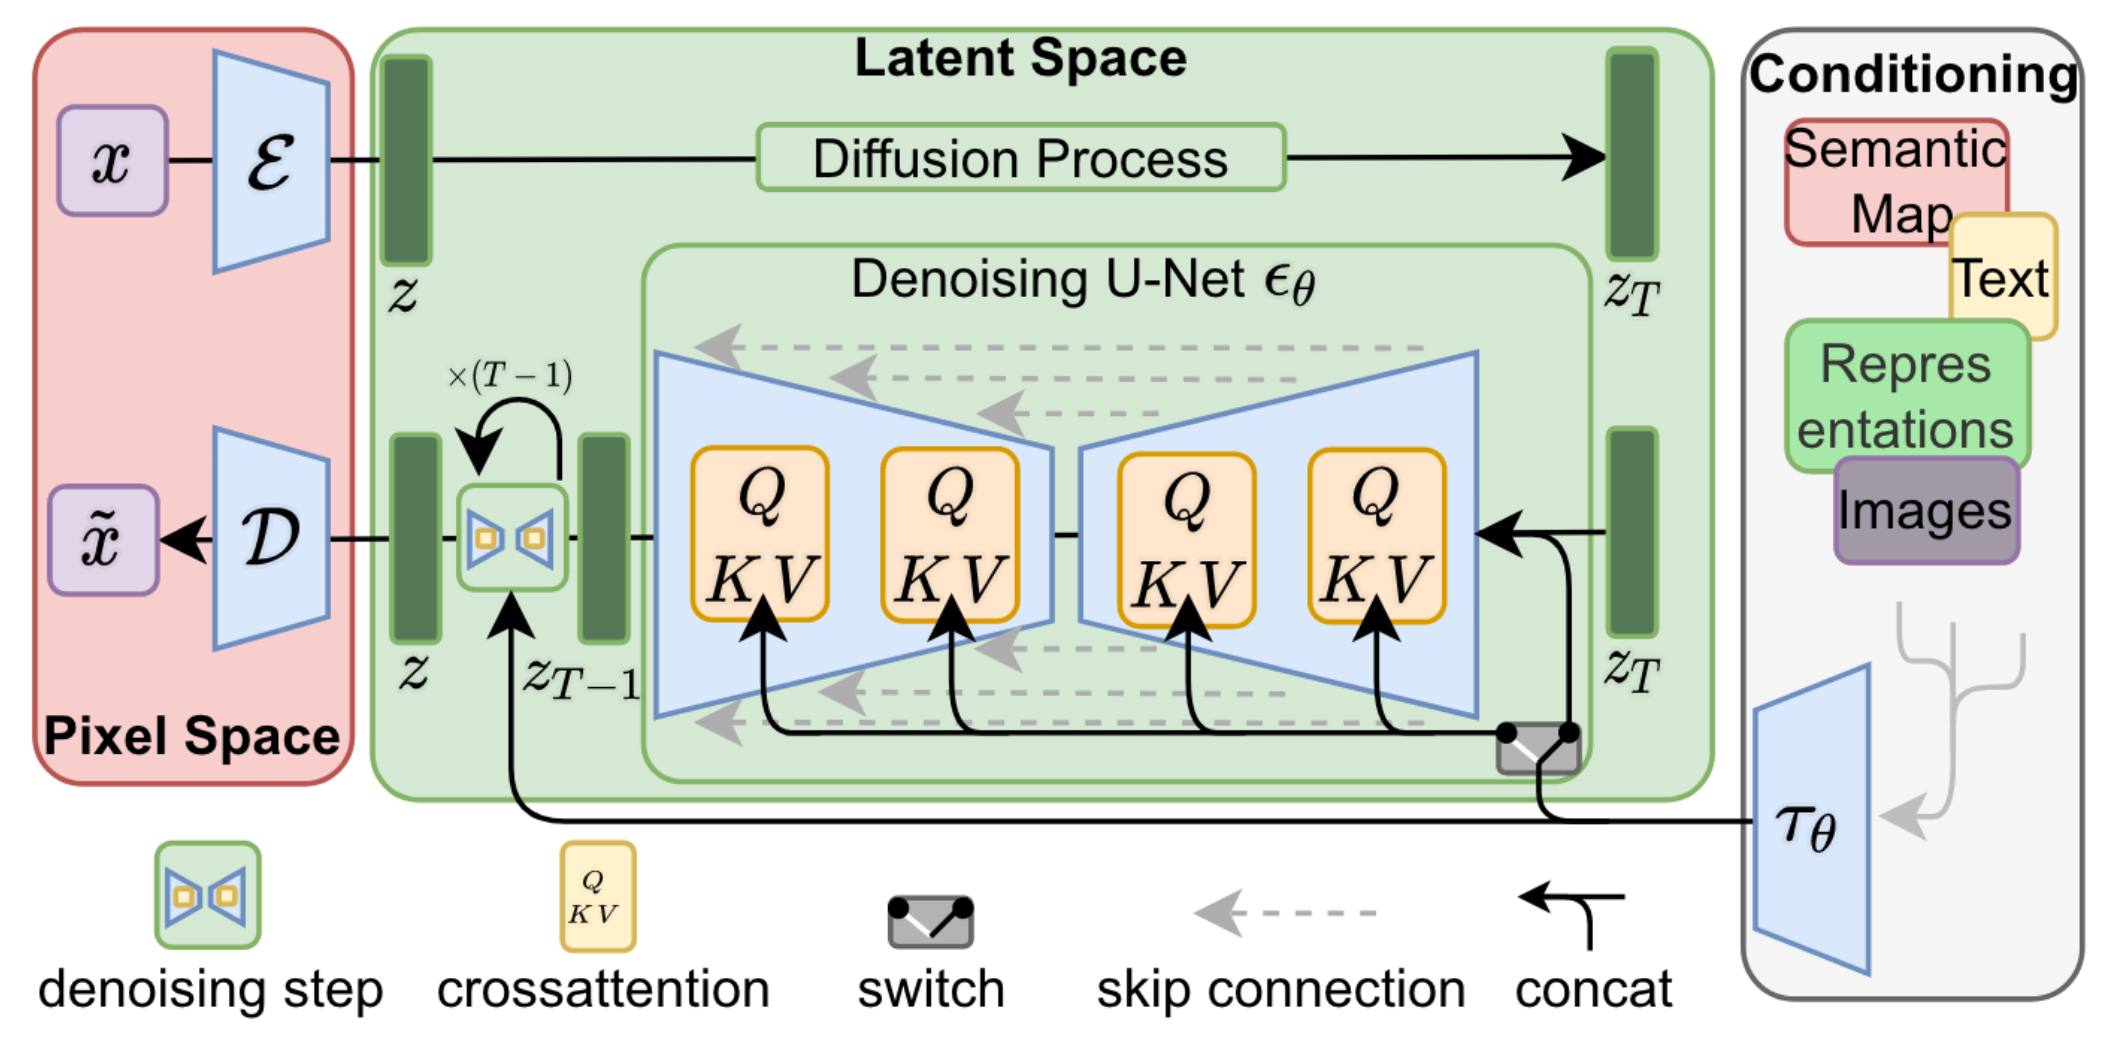
\includegraphics[width=.8\textwidth]{LDM.png}
  \caption[LDM Architektur]{LDM Architektur\cite{rombach_high-resolution_2022}}
  \label{fig:LDM}
\end{figure} 

Der latente Raum für den Diffusionsprozess wird durch vorausgehendes Training eines \emph{Variational Autoencoders} \cite{kingma_auto-encoding_2022} gemäß \cite{esser_taming_2021} erzeugt. Der resultierende \emph{Encoder} $\mathcal{E}$ transformiert ein RGB-Bild $x \in \mathbb{R}^{H \times W \times 3}$ in die latente Repräsentation $z \in \mathbb{R}^{h \times w \times c}$, so dass $z=\mathcal{E}(x)$. Ein \emph{Decoder} $\mathcal{D}$ generiert nach dem Rückwärtsdiffusionsprozess das Bild $\tilde{x}=\mathcal{D}(z)=\mathcal{D}(\mathcal{E}(x))$ \cite{rombach_high-resolution_2022}.

Der Diffusionsprozess profitiert von der niedrigen Dimensionalität und Kompression des latenten Raumes und zeigte sich gegenüber der Nutzung der originellen Pixelwerten als geeigneter für \emph{likelihood} basierte Generative Modelle, da mehr die semantischen wichtigen Information mehr zur Geltung kommen und der Rechenaufwand effizienter gehalten wird. Das zugrunde liegende \emph{U-Net} \cite{ronneberger_u-net_2015} besteht, um den Umgang mit Bildern gerecht zu werden, primär aus \emph{2D-Konvolutionsschichten}. \cite{rombach_high-resolution_2022}

Um die von einer Eingabe $y$ bedingten Generierung zu ermöglichen ist eine Konditionierung des Netzes $\epsilon_\theta\left(z_t, t, y\right)$ notwendig. Hierfür wird das benutze \emph{U-Net} um \emph{Cross Attention}\cite{vaswani_attention_2017} erweitert. Um die verschiedenen Eingabmodalitäten zu unterstützen verarbeiten zu können, schafft eine je nach Medium spezifischer Encoder $\tau_\theta$ eine Repräsentation $T_\theta(y) \in \mathbb{R}^{M \times d_\tau}$, welche mittels \emph{Cross Attention} $\operatorname{Attention}(Q, K, V)=\operatorname{softmax}\left(\frac{Q K^T}{\sqrt{d}}\right)$, mit $Q=W_Q^{(i)} \cdot \varphi_i\left(z_t\right), K=W_K^{(i)} \cdot \tau_\theta(y), V=W_V^{(i)} \cdot \tau_\theta(y)$ auf die Schichten des \emph{U-Net} übertragen wird. Die Verlustfunktion definert sich folgendermaßen. \cite{rombach_high-resolution_2022}

\begin{equation}
L_{L D M}:=\mathbb{E}_{\mathcal{E}(x), y, \epsilon \sim \mathcal{N}(0,1), t}\left[\left\|\epsilon-\epsilon_\theta\left(z_t, t, \tau_\theta(y)\right)\right\|_2^2\right]
\end{equation}


\subsection{Clap}

\emph{Large-Scale Contrastive Language-Audio Pretraining} (\emph{Clap})\cite{wu_large-scale_2023} präsentierte ein Modell, um Vortraining mittels \emph{Contrastive Learning} auf Sprach-Audio-Daten durchzuführen, mit dem Ziel, eine latente Repräsentation für Audio zu schaffen. Dieses Modell orientierte sich an der Architektur von \emph{Contrastive Language-Image Pretraining} (\emph{CLIP})\cite{radford_learning_2021}, bei dem in ähnlicher Weise ein Zusammenhang zwischen Bild und Textdaten erlernt wird. Analog zum bildlichen Kontext weisen Audio und Text überlappende Informationen auf. \cite{wu_large-scale_2023}

Das \emph{Contrastive Learning}-Modell wurde auf dem speziell veröffentlichten Datensatz \emph{LAION-Audio-630K} trainiert. Dieser Datensatz besteht aus $633,526$ Text- und Audio-Paaren ($X_i^a$, $X_i^t$), zusammengesetzt aus verschiedenen Internetquellen, einschließlich Klängen wie menschlichen Stimmen, Naturgeräuschen und Audioeffekten. Weitere verwendete Datensätze sind \emph{AudioCaps+Clotho} \cite{kim_audiocaps_2019} \cite{drossos_clotho_2019}, sowie \emph{AudioSet} \cite{gemmeke_audio_2017}. Alle Audiodaten werden zu einem \emph{Mono}-Signal konvertiert und besitzen eine Abtastrate von 48kHz. \cite{wu_large-scale_2023}

\begin{figure}[h]
  \centering
  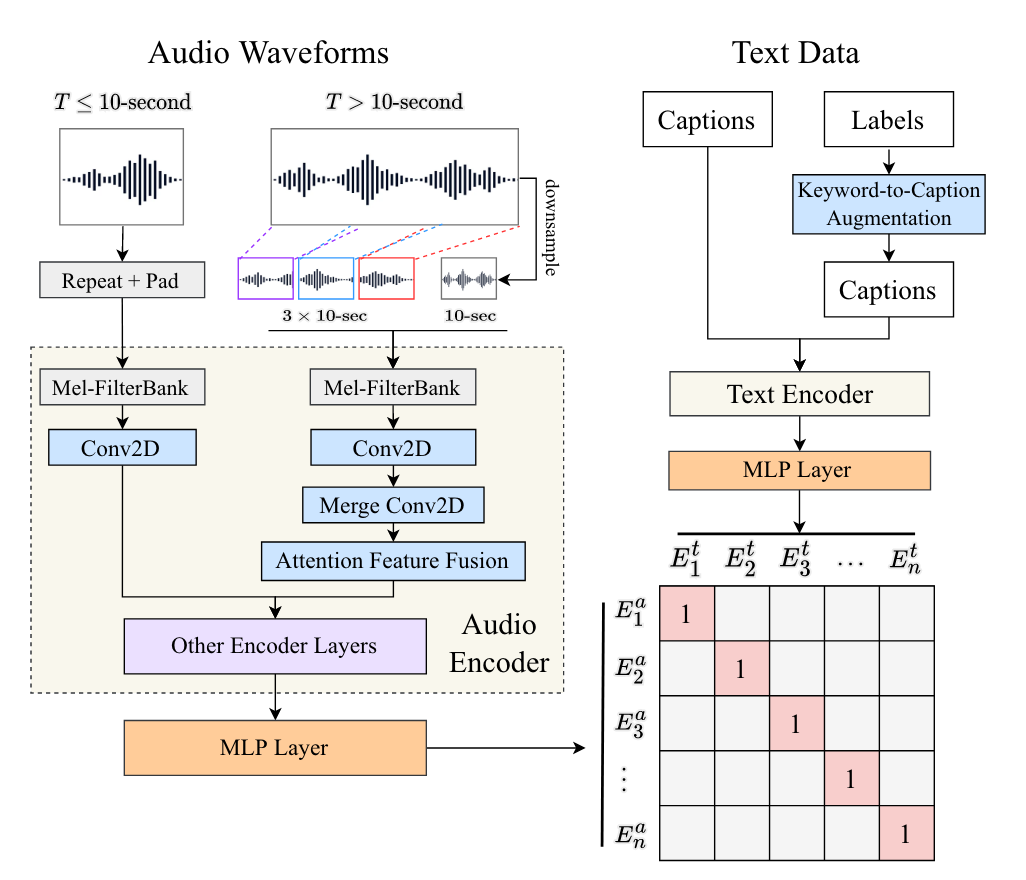
\includegraphics[width=.6\textwidth]{Clap.png}
  \caption[Clap Architektur]{CLAP Architektur \cite{wu_large-scale_2023}}
  \label{fig:Clap}
\end{figure} 

Die Architektur des Modells (Abbildung \ref{fig:Clap}) erzeugt Embeddings $E_i^a$, $E_i^t$ der Audio- $X_i^a$ und Texteingabe $X_i^t$, indem zuerst jeweils ein Encoder $f(\cdot)$ verwendet wird, dessen Ergebnis durch ein 2-Layer großes \emph{Multi-Layer-Perceptron} (\emph{MLP}) mit \emph{ReLU}\cite{agarap_deep_2019} als Aktivierungsfunktion verarbeitet wird. \cite{wu_large-scale_2023}

\begin{align}
  E_i^a & = M L P_{\text{audio}}\left(f_{\text{audio}}\left(X_i^a\right)\right) \\
  E_i^t & = M L P_{\text{text}}\left(f_{\text{text}}\left(X_i^t\right)\right)
\end{align}

Das gesamte Audiosignal zu encodieren, würde bei Signalen mit längerer Dauer zu viel Rechenzeit in Anspruch nehmen. Stattdessen wurde ein Ansatz verfolgt, bei dem verschiedene Längen von Audioeingaben in konstanter Rechenzeit trainiert und inferiert wurden. Hierzu wurden sowohl globale als auch lokale Informationen kombiniert. Falls das Signal kürzer als 10 Sekunden ist, wird es dreimal wiederholt und mit Nullen aufgefüllt, bis die 10 Sekunden erreicht sind. Wenn das Signal länger als 10 Sekunden ist, werden daraus vier Eingabeparameter generiert. Das Signal wird einmal komplett zu einem 10 Sekunden globalen Parameter \emph{downgesampled} und einmal werden drei zufällige 10 Sekunden Ausschnitte aus Anfang, Mitte und Ende des Signals als lokale Parameter entnommen. Der Audio-Encoder extrahiert anschließend die wichtigen Informationen und verschmilzt globale und lokale Informationen.

Da einige der verwendeten Datensätze keine Beschreibungen, sondern nur Keywords oder Tags für das jeweilige Audiosignal besitzen, wurde das \emph{Language}-Modell \emph{T5}\cite{raffel_exploring_2020} eingesetzt, um vollständige Beschreibungen aus den Keywords und Tags zu generieren. Auch wurden die Beschreibungen \emph{de-biased}, beispielsweise durch \emph{gender de-biasing}. \cite{wu_large-scale_2023}

Die gleiche Verlustfunktion mit einem Temperaturparameter $\tau$, wie in \emph{Clip}\cite{radford_learning_2021}, wurde in den MLPs verwendet \cite{wu_large-scale_2023}.

\begin{equation}
L=\frac{1}{2 N} \sum_{i=1}^N\left(\log \frac{\exp \left(E_i^a \cdot E_i^t / \tau\right)}{\sum_{j=1}^N \exp \left(E_i^a \cdot E_j^t / \tau\right)}+\log \frac{\exp \left(E_i^t \cdot E_i^a / \tau\right)}{\sum_{j=1}^N \exp \left(E_i^t \cdot E_j^a / \tau\right)}\right)
\end{equation}

Als Audio-Encoder wurden die Modelle \emph{PANN}\cite{kong_panns_2020}, basierend auf einem \emph{Convolutional Neural Network} (CNN), und \emph{HTSAT}\cite{chen_hts-at_2022}, basierend auf einem \emph{Transformer}-Modell, evaluiert. Für den Text-Encoder wurden der Text-Encoder von \emph{Clip}\cite{radford_learning_2021}, \emph{Bert}\cite{devlin_bert_2019}, oder \emph{RoBERTa}\cite{liu_roberta_2019} ebenfalls ausgewertet. \cite{wu_large-scale_2023}

Das trainierte Modell kann für Audio-Klassifikation verwendet werden oder ein passendes Audiosignal für einen Text bestimmen $(T\rightarrow A)$ \cite{wu_large-scale_2023}. Für die Klangsynthese ist der Prozess von Text zu Audio von Bedeutung. Die Ergebnisse der Kombination der verschiedenen Encoder aus Tabelle \ref{tab:Clap} zeigen, dass \emph{HTSAT}\cite{chen_hts-at_2022} als Audio-Encoder und je nach Datensatz \emph{Bert}\cite{devlin_bert_2019} oder \emph{RoBERTa}\cite{liu_roberta_2019} als Text-Encoder die besten Resultate lieferten. \cite{wu_large-scale_2023}

\begin{table}[h]
  \centering
\begin{tabular}{lcc|cc}
\hline \multirow{2}{*}{ Model } & \multicolumn{2}{c|}{ AudioCaps $(\mathrm{mAP} @ 10)$} & \multicolumn{2}{c}{ Clotho (mAP@ 10) } \\
\cline { 2 - 5 } & $\mathrm{A} \rightarrow \mathrm{T}$ & $\mathrm{T} \rightarrow \mathrm{A}$ & $\mathrm{A} \rightarrow \mathrm{T}$ & $\mathrm{T} \rightarrow \mathrm{A}$ \\
\hline PANN+CLIP Trans. & 4.7 & 11.7 & 1.9 & 4.4 \\
PANN+BERT & 34.3 & 44.3 & 10.8 & 17.7 \\
PANN+RoBERTa & 37.5 & 45.3 & 11.3 & 18.4 \\
HTSAT+CLIP Trans. & 2.4 & 6.0 & 1.1 & 3.2 \\
HTSAT+BERT & 43.7 & 49.2 & $\mathbf{1 3 . 8}$ & $\mathbf{2 0 . 8}$ \\
HTSAT+RoBERTa & $\mathbf{4 5 . 7}$ & $\mathbf{5 1 . 3}$ & $\mathbf{1 3 . 8}$ & 20.4 \\
\hline
\end{tabular}
\caption[Encoder CLAP]{Evaluation der Encoder \cite{wu_large-scale_2023}}
  \label{tab:Clap}
\end{table}


\subsection{AudioLDM}

Das Modell \emph{AudioLDM}\cite{liu_audioldm_2023-1} dient zur Synthese von Text zu Audio sowie zur textgesteuerten Audio-Manipulation mittles \emph{Latenten Diffusion}\cite{rombach_high-resolution_2022}. Es verspricht qualitativ hochwertige Ergebnisse bei geringem Rechenaufwand. Im Gegensatz zu \emph{Diffsound}\cite{yang_diffsound_2023}, das Audio-Text-Paare für das Training verwendet, hat \emph{AudioLDM} gezeigt, dass mithilfe einer \emph{CLAP}-Repräsentation\cite{wu_large-scale_2023} hochwertige Resultate erzielt werden können. \cite{liu_audioldm_2023-1}

Die Wahl, Natürliche Sprache anstelle von Labels für die Eingabe und Konditionierung zu verwenden, erfolgte aufgrund der Möglichkeit, akustische Merkmale flexibler, deskriptiver und präziser darzustellen. Frühere Ansätze im Bereich Text-zu-Audio (TTA) stießen auf die Grenze, dass oft keine großen Mengen qualitativ hochwertiger Audio-Text-Daten verfügbar waren\cite{liu_separate_2022}. Methoden der Textvorverarbeitung\cite{gemmeke_audio_2017, yang_diffsound_2023} konnten dieses Problem nicht gänzlich lösen, da sie komplexe Zusammenhänge zwischen Klangereignissen vereinfachten, was die Generierungsleistung beeinträchtigte. Das Modell \emph{AudioLDM} adressierte diese Herausforderung, indem es ausschließlich auf Audiodaten im Training setzte und so bessere Ergebnisse erzielte als mit gepaarten Audio-Text-Daten. \cite{liu_audioldm_2023-1}


\begin{figure}[h]
  \centering
  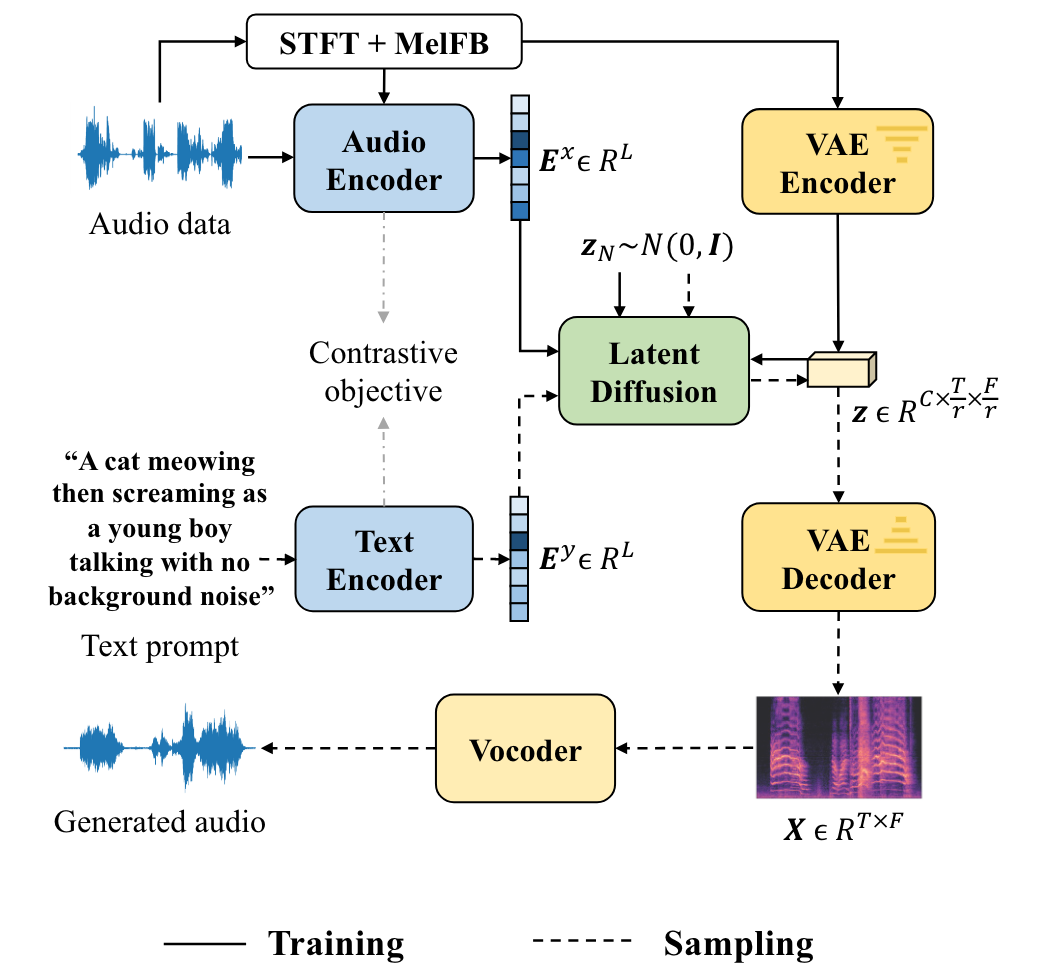
\includegraphics[width=.6\textwidth]{AudioLDM.png}
  \caption[AudioLDM Architektur]{Architektur für die Text-Generierung von AudioLDM\cite{liu_audioldm_2023-1}}
  \label{fig:AudioLDM}
\end{figure} 

Die Architektur (Abbildung \ref{fig:AudioLDM}) kombiniert mehrere Komponenten: Einen \emph{VAE}\cite{kingma_auto-encoding_2022}, der Mel-Spektrogramme in einen latenten Raum kodiert; einen nach \emph{CLAP}\cite{wu_large-scale_2023} konzipierten Audio- und Text-Encoder, der Embeddings für die Konditionierung des \emph{LDMs} erstellt; einen \emph{LDM}, der die zugrunde liegende Verteilung erlernt; und einen \emph{Vocoder}, der das generierte Spektrogramm in ein Audiosignal umwandelt. \cite{liu_audioldm_2023-1}

Die \emph{CLAP}-Module generieren Embeddings für Text $\boldsymbol{E}^y \in \mathbb{R}^L$ und Audio $\boldsymbol{E}^x \in \mathbb{R}^L$. Hierbei repräsentiert $x$ eine Audioprobe und $y$ eine Textbeschreibung, wobei jeweils $f_{\text {text }}(\cdot)$ und $f_{\text {audio }}(\cdot)$ als Encoder dienen. Für den Audioencoder wurde \emph{HTSAT}\cite{chen_hts-at_2022} und für den Textencoder \emph{RoBERTa}\cite{liu_roberta_2019} verwendet. Beim Training des \emph{LDMs} diente $\boldsymbol{E}^x$ aus dem jeweiligen Trainingsdatenpunkt als Konditionierung, während $\boldsymbol{E}^y$ zur Generierung des gewünschten Signals Verwendung findet. \cite{liu_audioldm_2023-1}

Für den \emph{LDM}-genutzten Latentraum $\boldsymbol{z} \in \mathbb{R}^{C \times \frac{T}{r} \times \frac{F}{r}}$ fand ein Training mithilfe eines \emph{VAE} auf Spektrogrammen statt. Dabei repräsentiert $r$ das \emph{Kompressionslevel}, während $T$ und $F$ für Zeit- und Frequenzdimensionen stehen. $C$ gibt die Anzahl der Kanäle an. Ein Spektrogramm $\boldsymbol{X} \in \mathbb{R}^{T \times F}$ wird durch \emph{STFT} (Referenz \ref{sec:music_math}) aus einem gegebenen Audiosignal generiert. Im Generierungsverfahren wird aus der latenten Variable $\hat{\boldsymbol{z}}_o$ ein Spektrogramm $\hat{\boldsymbol{X}}$ erstellt. Dieses Spektrogramm wird schließlich durch den \emph{Vocoder}, basierend auf \emph{HiFi-GAN}\cite{kong_hifi-gan_2020}, in ein Audiosignal $\hat{x}$ transformiert. \cite{liu_audioldm_2023-1}

Das konzeptionelle \emph{LDM} hat das Ziel, die grundlegende Verteilung $q\left(\boldsymbol{z}0 \mid \boldsymbol{E}^y\right)$ mithilfe von $p\theta\left(\boldsymbol{z}_0 \mid \boldsymbol{E}^y\right)$ anzunähern. Dabei wurden Verlustfunktion und der Rückwärtsprozess wie folgt spezifiziert: \cite{liu_audioldm_2023-1}

\begin{equation}
    L_n(\theta)=\mathbb{E}_{\boldsymbol{z}_0, \boldsymbol{\epsilon}, n}\left\|\boldsymbol{\epsilon}-\boldsymbol{\epsilon}_\theta\left(\boldsymbol{z}_n, n, \boldsymbol{E}^x\right)\right\|_2^2
\end{equation}
\begin{equation}
    p_\theta\left(\boldsymbol{z}_{n-1} \mid \boldsymbol{z}_n, \boldsymbol{E}^y\right)=\mathcal{N}\left(\boldsymbol{z}_{n-1} ; \boldsymbol{\mu}_\theta\left(\boldsymbol{z}_n, n, \boldsymbol{E}^y\right), \boldsymbol{\sigma}_n^2 \boldsymbol{I}\right)
\end{equation}
\begin{equation}
    p_\theta\left(\boldsymbol{z}_{0: N} \mid \boldsymbol{E}^y\right)=p\left(\boldsymbol{z}_N\right) \prod^N p_\theta\left(\boldsymbol{z}_{n-1} \mid \boldsymbol{z}_n, \boldsymbol{E}^y\right) \\
\end{equation}

Der Erwartungswert ist folgendermaßen parametrisiert und berechnet sich aus dem im Rückwärtsprozess ermittelten Rauschen $\boldsymbol{\epsilon}_\theta\left(\boldsymbol{z}_n, n, \boldsymbol{E}^y\right)$ \cite{liu_audioldm_2023-1}.

\begin{equation}
    \boldsymbol{\mu}_\theta\left(\boldsymbol{z}_n, n, \boldsymbol{E}^y\right)=\frac{1}{\sqrt{\alpha_n}}\left(\boldsymbol{z}_n-\frac{\beta_n}{\sqrt{1-\bar{\alpha}_n}} \boldsymbol{\epsilon}_\theta\left(\boldsymbol{z}_n, n, \boldsymbol{E}^y\right)\right)
\end{equation}

Des weiterem wurde gezeigt, dass der \emph{Cross-Attention}-Mechanismus aus \cite{rombach_high-resolution_2022} weggelassen werden kann \cite{liu_audioldm_2023-1}. 

\section{Implementierung des Neuronalen Synthesizers}
\subsection{Audioprogrammierung}
Die Geschwindigkeit der Datenverarbeitung stellt ein maßgebliches Kriterium bei der Wahl der Programmiersprache für die Entwicklung und Implementierung von digitalen Audioprozessen dar. Für Echtzeitanwendungen gilt insbesondere, dass der Code so effizient wie möglich gestaltet sein sollte, um jegliche Latenz zu minimieren. Unter Berücksichtigung dieser Prämissen fällt die Wahl häufig auf eine Realisierung in \emph{C/C++}. \cite{doumler_c_2015, boulanger_audio_2011}

C++ entstand als Erweiterung der Sprache C und behält dabei C als seine Untermenge. Es stützt sich auf die Grundprinzipien von C, insbesondere die hardwarenahe Programmiermöglichkeit und die Tatsache, dass C auf den meisten Systemen laufen kann. Darüber hinaus bereichert C++ das Spektrum um Aspekte der Datenabstraktion sowie objektorientierte und generische Programmierparadigmen. \cite{stroustrup_c_1997}
\subsection{JUCE Framework}
\glqq\emph{JUCE} ist das am häufigsten verwendete Framework für die Entwicklung von Audioanwendungen und -Plugins. Es handelt sich dabei um eine Open-Source-C++-Codebasis, die zur Erstellung eigenständiger Software auf Windows, macOS, Linux, iOS und Android sowie VST-, VST3-, AU-, AUv3-, AAX- und LV2-Plugins verwendet werden kann.\grqq \cite{noauthor_juce_nodate-1}

Es bietet eine Abstraktion für die Verarbeitung von Audiosamples und MIDI von den nativen Audiogeräten auf jeder Plattform oder einer Host-DAW. Mit der Bibliothek von \emph{digitalen Signalverarbeitungs-(DSP)-Bausteinen}, die JUCE bereitstellt, können unterschiedliche Audioeffekte, Filter, Instrumente und Generatoren schnell prototypisiert und eingesetzt werden. \cite{noauthor_juce_nodate-1} So umfasst wa eine breite Palette von Klassen, die häufig auftretende Probleme bei der Entwicklung von Audioprojekten lösen. Dazu gehören die Behandlung von Grafiken, Sound, Benutzerinteraktion und Netzwerken. \cite{robinson_getting_2013}

In dieser Arbeit wird das JUCE-Framework mittels \emph{CMake}, \glqq eine Open-Source-, plattformübergreifende Werkzeugfamilie, die zur Erstellung, zum Testen und zum Verpacken von Software entwickelt wurde\grqq \cite{noauthor_cmake_nodate} benutzt, um die durch das Diffusionsnetz erstellten Klänge spielbar und manipulierbar zu gestalten. 

Das Juce Module \emph{PluginGuiMagic} \cite{walz_plugin_nodate} ermöglicht die Erstellung einer Benutzeroberfläche für die zu entwickelnde Anwendung zu vereinfachen und zu beschleunigen. 


\subsection{AudioLDM-Anbindung} \label{sec:api}
Um die Wiedergabe eines vom Diffusionsmodell generierten Samples im Synthesizer zu realisieren, ist es notwendig, das Modell in den C++-Quellcode zu integrieren. Hierfür existieren prinzipiell drei mögliche Methoden zur Implementierung von AudioLDM. Eine optimal anmutende Herangehensweise wäre die Konvertierung des trainierten Modells in ein \emph{ONNX}-Modell \cite{noauthor_onnx_nodate-1}, wodurch eine binäre Repräsentation des Modells entstehen würde. Mit Hilfe der \emph{ONNX-Runtime} \cite{noauthor_onnx_nodate} könnte diese dann in C++ eingebettet und geladen werden, um Inferenzoperationen durchzuführen und somit die Generierung von Sound zu ermöglichen. Diese Vorgehensweise würde besonders das Zusammenstellen und die Verbreitung des fertiggestellten Instruments inklusive des trainierten Modells begünstigen. Eine alternative Option wäre die Konvertierung des Modells in ein \emph{Torchscript}-Modell \cite{noauthor_torchscript_nodate} und das anschließende Laden in C++. \cite{oli_larkin_machine_2023} 

Aktuell konnte jedoch weder ein ONNX- noch ein Torchscript-Modell für das AudioLDM-Modell generiert werden, da dieses aus einem komplexen Zusammenspiel verschiedener Modelle und Module besteht und einige der eingesetzten Modelle und Module derzeit noch nicht von ONNX oder Torchscript unterstützt werden. Ausdiesem Grund wurde für die Umsetzung dieses Projekts die Entwicklung einer \emph{API (Application Programming Interface)} gewählt, durch die über definierte Endpunkte eine lokale Instanz des Modells erzeugt und zur Generierung der benötigten Samples verwendet werden kann. Als Framework für diese Implementierung kommt \emph{FastAPI} \cite{noauthor_fastapi_nodate} zum Einsatz. Auf dem Python-Server wird eine Instanz des AudioLDM-Modells ausgeführt. Diese wird als \emph{Pipeline} durch die \emph{Diffusers} Bibliothek von \emph{Huggingface} \cite{noauthor_huggingface_nodate} verwendet. Der Einsatz dieser Pipeline ermöglicht die Durchführung von Inferenzen mit einem gewissen Grad an Abstraktion und eine Anwendung auf verschiedenen Systemen. So war das veröffentlichte Modell ursprünglich nicht auf Computern ohne GPU, wie den M-Modellen von Apple, lauffähig. Durch die Möglichkeit, den zu verwendenden Prozessor innerhalb der Pipeline festzulegen, konnte dieses Problem jedoch behoben werden. Des Weiteren erlaubt die Nutzung einer API, dass bei mehreren Instanzen des Synthesizers nicht für jede ein neues Modell initialisiert werden muss, was das parallele Betreiben mehrerer Modelle vermeidet.

Die implementierten Endpunkte umfassen einen zur Initialisierung eines Modells, der das \emph{Gerät} (auf welchem Prozessor die Berechnung ausgeführt werden soll) und das \emph{Modell} (bestimmt, welches vortrainierte Modell verwendet werden soll) benötigt. Der Endpunkt zur Generierung eines Klangs erfordert einen \emph{Prompt}, \emph{negativen Prompt}, die \emph{Audiolänge}, \emph{Anzahl der Inferenzschritte} sowie eine \emph{Leitskala} und liefert ein in \emph{Base64} kodiertes Audiosignal zurück.

\begin{figure}
  \centering
  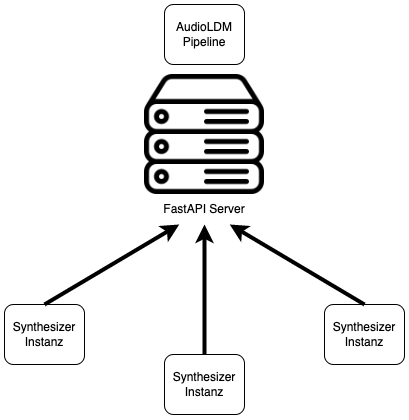
\includegraphics[width=.4\textwidth]{graphics/Server.png}
  \caption[Infrastruktur]{Anbindung an den AudioLDM Server}
  \label{fig:server}
\end{figure}

\subsection{Sampler}

Für die Implementierung des Samplers wurde der bereits von \emph{Juce}\cite{noauthor_juce_nodate-1} zur Verfügung gestellte Sampler \cite{noauthor_juce_nodate} verwendet. Zusätzlich wurde die Funktionalität erweitert, um eine spezifische Tonverschiebung vornehmen zu können und den Pitch-Bender an einem Keyboard einsetzen zu können.

\chapter{Ergebnisse}
Das Zusammenspiel der vorgestellten Komponenten und Elemente führte zu einem digitalen Instrument, welches als Standalone oder als Plugin in einem VST3 oder AU-Format in einer DAW wie \emph{Ableton} \cite{noauthor_ableton_nodate}, \emph{Logic} \cite{noauthor_logic_nodate} und anderen, unter Windows und Mac, verwendet werden kann.

\begin{figure}[h]
  \centering
  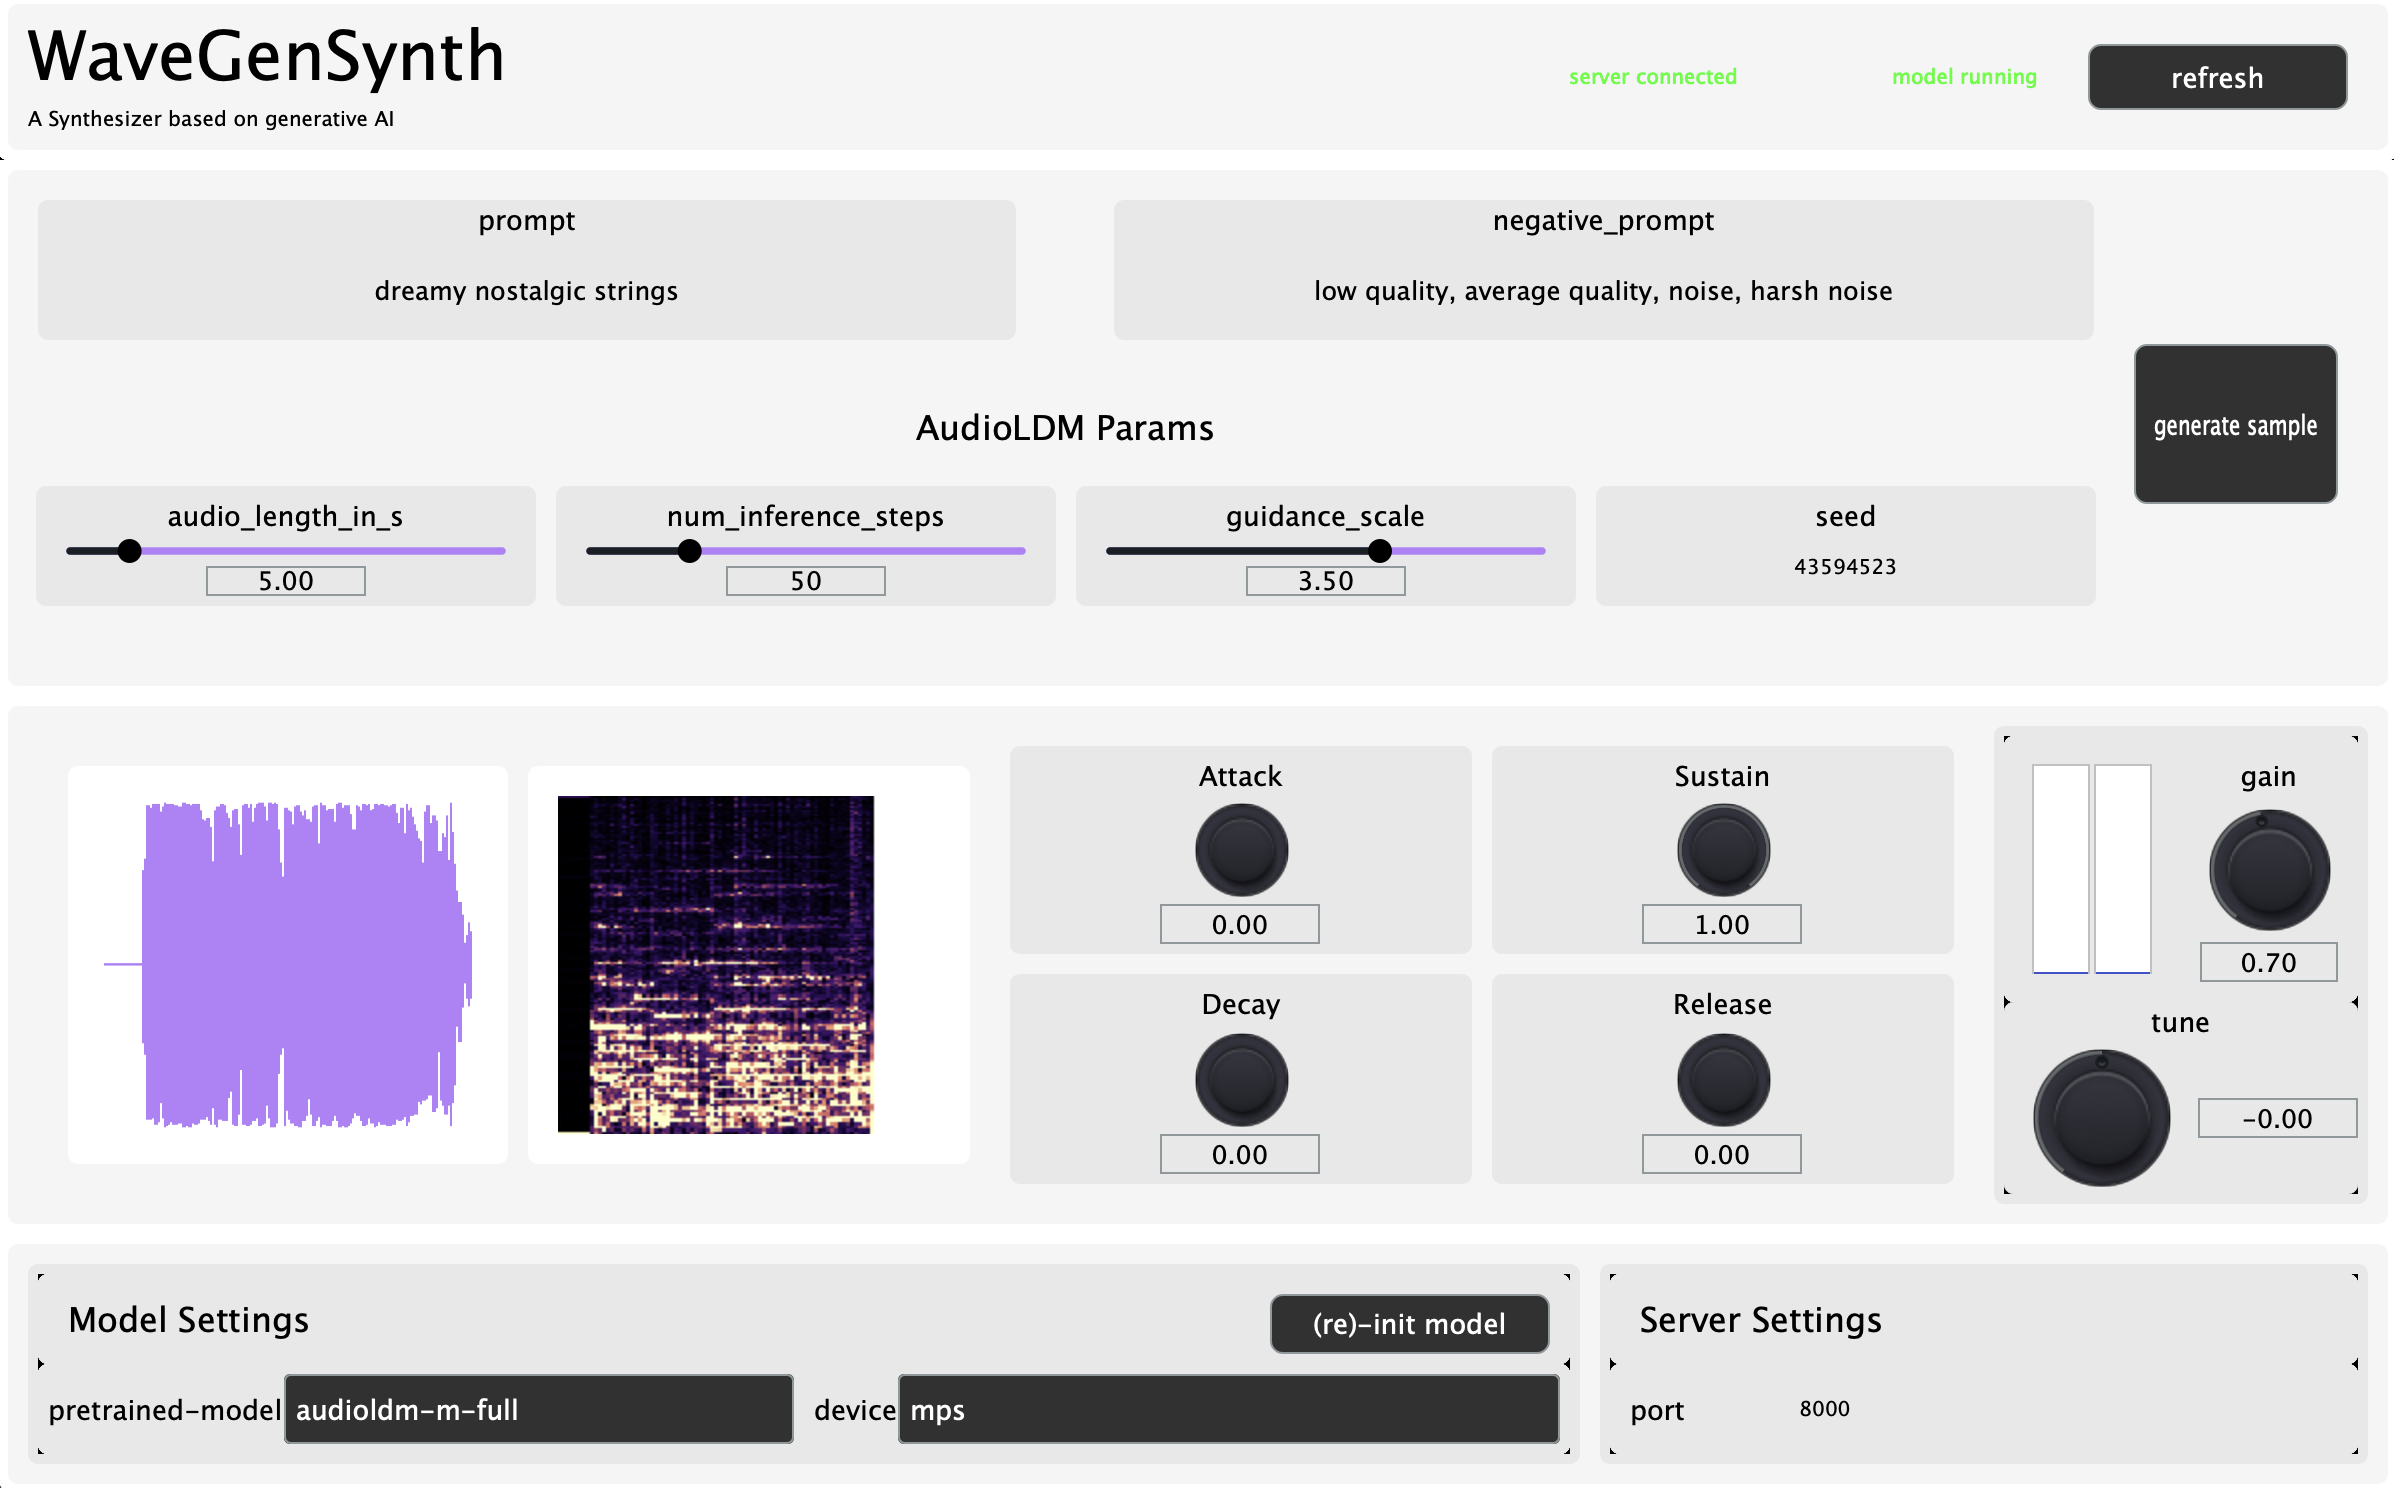
\includegraphics[width=1.0\textwidth]{synth.png}
  \caption[Benutzeroberfläche]{Benutzeroberfläche}
  \label{fig:synth}
\end{figure} 

Die daraus entstandene Benutzeroberfläche (Abbildung \ref{fig:synth}) ermöglicht es einem Nutzer, den Server für die API (siehe \ref{sec:api}) auf einem gewünschten Port  zu starten und ein Modell zu initiieren, indem aus einer Auswahl von vorab trainierten Modellen gewählt wird. Die Verwendung des Modells auf verschiedenen Hardwarekonfigurationen (mit und ohne GPU) und Betriebssystemen wird durch die Auswahl an unterstützten Geräten ermöglicht. Nach der Initialisierung eines Modells kann ein gewünschter Klang, der durch die Texteingabefelder \emph{Prompt} und \emph{Negative Prompt} definiert wird, synthetisiert werden. Auch die Länge des zu erzeugenden Klangs in Sekunden (\emph{audio length}), die Anzahl der Inferenzschritte (\emph{number of inference steps}) und die Leitskala (\emph{guidance scale}) lassen sich einstellen. Um die Erzeugung determiniert zu machen, kann auch ein \emph{Seed} in Form eines 8-Byte großen Integers im Wertebereich von $0$ bis $2^{64}-1$ mit angegeben werden.  

Die \emph{Hüllkurve} des \emph{Samplers} (siehe \ref{sec:synth+envelope}) lässt sich über vier Parameter modifizieren. Hierbei sind die Zeitspannen in Sekunden für die Anschwell- (engl. \emph{attack}), Abschwell- (engl. \emph{decay}) und Ausschwingphasen (engl. \emph{release}) sowie das Level, auf das die Lautstärke absinken soll (engl. \emph{sustain}), festlegbar. Der von dem Instrument generierte Klang kann mithilfe des Sliders "Verstärkung" (engl. \emph{gain}) auf eine bestimmte Lautstärke angepasst werden.

Da die Tonhöhe des generierten Klangs nicht im Voraus bestimmt werden kann und der Klang standardmäßig der \emph{Midi}-Note $C4$ zugeordnet wird, besteht die Möglichkeit, das Instrument so zu stimmen, dass die Tonhöhe des Klangs der gespielten Note entspricht. Hierbei kann der Klang kontinuierlich um bis zu zwölf Halbtöne, also einer Oktave, nach oben oder unten angepasst werden.

Das produzierte Signal wird durch eine Wellenform- und Spektrogramm-Anzeige visualisiert. Dies soll dem Nutzer dabei helfen, die Ergebnisse des Modells besser nachzuvollziehen und das erfolgreiche Generieren zu erkennen. Zudem lassen sich aus dieser Visualisierung bestimmte Klangstrukturen herauslesen.

Die Soundqualität des Instrumentes und die Fähigkeit die gewünschten musikalischen Merkmale aus der textuellen Eingabe zu generieren hängt von dem zur Verwendung kommenden Modell ab.    Genauigkeit des 

//TODO: Ergebnisse von AudioLDM im musikalischen Kontext, und wie gut es Sound für die Musikproduktion erziehelen kann. 

\chapter{Diskussion}

Das Aufzeigen, der Möglichkeit Instrumente basierend auf künstlicher Intelligenz zu entwickeln stellt eine beachtliche Erweiterung der musikalischen Klangerzeugung dar. Neue Arten Klänge oder Musik zu erzeugen, manipulieren oder zu spielen  


Schwächen:

AudioLDM

Zu wenig Training über Musikproduktions Keywords

Nervige Obertöne

Keine zuordnung zu Genres, Künstler, Epochen

Keine Automatische Pitch Erkennung

--------------

Stärken:

Neue Soundsynthese

Ambiend Pads

Sound Experimentierung

Happy Little Accidents


--------------

Verbesserung:

Automatische Pitch Zuordnung

Mehr Zuordnung zu Emotionen 

AudioLDM 2

Schneller Inferenz

Spezielle Hardware 

ML-Sampler

Spektogramm Manipulation 

Loop Points

Modulare Aufbau 

Finetuning auf mehr musikalischen Daten

Indivduelles Finetuning 

Eine Programmiersprache

ONNX

Binäredaten

Envelope Visualiesieren

Additive Synth

Convelution Mixer

Presets speichern 

Schon Präsente Spuren Analysieren und Lücken finden 

ML-Effekte

Mehre Modell Auswahl 

Modell zusammenbauen ? 





\chapter{Schlussfolgerung}
\label{sec:conclusion}


\printbibliography

All links were last followed on \today{}.

\appendix
%% !TeX root = main-english.tex
% !TeX spellcheck = en-US
% !TeX encoding = utf8
% -*- coding:utf-8 mod:LaTeX -*-

%This smart spell only works if no changes have been made to the chapter 
%using the options proposed in preambel/chapterheads.tex.
\setchapterpreamble[u]{%
  \dictum[Albert Einstein]{We cannot solve our problems with the same level of thinking that created them}
}
\chapter{LaTeX Hints}
\label{chap:latexhints}

One sentence per line.
This rule is important for the usage of version control systems.
A new line is generated with a blank line.
As you would do in Word:
New paragraphs are generated by pressing enter.
In LaTeX, this does not lead to a new paragraph as LaTeX joins subsequent lines.
In case you want a new paragraph, just press enter twice (!).
This leads to an empty line.
In word, there is the functionality to press shift and enter.
This leads to a hard line break.
The text starts at the beginning of a new line.
In LaTeX, you can do that by using two backslashes (\textbackslash\textbackslash).
This is rarely used.

Please do \textit{not} use two backslahes for new paragraphs.
For instance, this sentence belongs to the same paragraph, whereas the last one started a new one.
A long motivation for that is provided at \url{http://loopspace.mathforge.org/HowDidIDoThat/TeX/VCS/#section.3}.

One can write \emph{emphasized text (rendered in italics)} and \textbf{bold text}.

\section{File Encoding and Support of Umlauts}
\label{sec:firstsectioninlatexhints}
The template offers foll UTF-8 support.
All recent editors should not have issues with that.

\section{Citations}


References are set by means of \texttt{\textbackslash cite[key]}.

\begin{filecontents*}{\democodefile}
Example: \cite{WSPA} or by author input: \citet{WSPA}.
\end{filecontents*}
\PrintDemo{style=parallel}

The following sentence demonstrates
\begin{inparaenum}[1.]
  \item the capitalization of author names at the beginning of the sentence,
  \item the correct citation using author names and the reference,
  \item that the author names are a hyperlink to the bibliography and that
  \item the bibliography contains the name prefix \qq{van der} of \qq{Wil M.\,P.\ van der Aalst}.
\end{inparaenum}

\begin{filecontents*}{\democodefile}
\Citet{RVvdA2016} present a study on the effectiveness of workflow management systems.
\end{filecontents*}
\PrintDemo{style=parallel}

The following sentence demonstrates that you can overwrite the text part of the generated label using \texttt{label} in a bibliopgrahie"=entry, but the year and the uniqueness is still generated by biber.

\begin{filecontents*}{\democodefile}
The workflow engine Apache ODE \cite{ApacheODE} executes \BPEL processes reliably.
\end{filecontents*}
\PrintDemo{style=parallel}

\begin{filecontents*}{\democodefile}
Words are best enclosed using \texttt{\textbackslash qq\{..\}}, then the correct quotes are used.
\end{filecontents*}
\PrintDemo{style=parallel}

When creating the Bibtex file it is recommended to make sure that the DOI is listed.

\section{Formulas and Equations}
\label{sec:mf}

\begin{filecontents*}{\democodefile}
Equations $f(x)=x$ inside the text can be provided.
\end{filecontents*}
\PrintDemo{style=parallel}

A list with all available mathematical symbols is provided at \url{http://texdoc.net/pkg/symbols-a4}.

\begin{filecontents*}{\democodefile}
As example the set of natural numbers is given by $\mathbb{N}$.
\end{filecontents*}
\PrintDemo{style=parallel}

For the documentation of editing mathematical formulas read the package documentation of \texttt{amsmath}\footnote{\url{http://texdoc.net/pkg/amsmath}}.

Equation~\ref{eq:test} is numbered and can be referenced in the text:
\begin{filecontents*}{\democodefile}
\begin{align}
  \label{eq:test}
  x = y
\end{align}
\end{filecontents*}
\PrintDemo{style=parallel}

Following equation is not numbered because of using \texttt{\textbackslash align*} as environment.
\begin{filecontents*}{\democodefile}
\begin{align*}
  x = y
\end{align*}
\end{filecontents*}
\PrintDemo{style=parallel}

The template offers \verb+\abs+ to enable the bars scaling well at the absolute value:

\begin{filecontents*}{\democodefile}
$\abs{X}$.
\end{filecontents*}
\PrintDemo{style=parallel}

More details about mathematical environments provides the documentation available at \url{http://www.ctan.org/tex-archive/help/Catalogue/entries/voss-mathmode.html}.


%%%%%%%%%%%%%%%%%%%%%%%%%%%%%%%%%%%%%%%%%%%%%%%%%%%%%%%%%%%%%%%%%%%%%%%%%%%%%%
\section{Sourcecode}
%%%%%%%%%%%%%%%%%%%%%%%%%%%%%%%%%%%%%%%%%%%%%%%%%%%%%%%%%%%%%%%%%%%%%%%%%%%%%%
\Cref{lst:ListingANDlstlisting} shows how to emmbed source code.
With \texttt{\textbackslash lstinputlisting} the source code can be loaded directly from files.

%Listing-Umgebung wurde durch \newfloat{Listing} definiert
\begin{Listing}
  \begin{lstlisting}
<listing name="second sample">
  <content>not interesting</content>
</listing>
\end{lstlisting}
  \caption{The code is separated by two horizontal lines in the listings environment.}
  \label{lst:ListingANDlstlisting}
\end{Listing}

\begin{filecontents*}{\democodefile}
Source code is also available in the text \lstinline|<listing />|.
\end{filecontents*}
\PrintDemo{style=parallel}


%%%%%%%%%%%%%%%%%%%%%%%%%%%%%%%%%%%%%%%%%%%%%%%%%%%%%%%%%%%%%%%%%%%%%%%%%%%%%%
\section{Pseudocode}
%%%%%%%%%%%%%%%%%%%%%%%%%%%%%%%%%%%%%%%%%%%%%%%%%%%%%%%%%%%%%%%%%%%%%%%%%%%%%%
\Cref{alg:sample} shows a sample algorithm.
\begin{Algorithmus} %Use the environment only if you want to place the algorithm similar to graphics from TeX
  \caption{Sample algorithm}
  \label{alg:sample}
  \begin{algorithmic}
\Procedure{Sample}{$a$,$v_e$}
\State $\mathsf{parentHandled} \gets (a = \mathsf{process}) \lor \mathsf{visited}(a'), (a',c,a) \in \mathsf{HR}$
\State \Comment $(a',c'a) \in \mathsf{HR}$ denotes that $a'$ is the parent of $a$
\If{$\mathsf{parentHandled}\,\land(\mathcal{L}_\mathit{in}(a)=\emptyset\,\lor\,\forall l \in \mathcal{L}_\mathit{in}(a): \mathsf{visited}(l))$}
\State $\mathsf{visited}(a) \gets \text{true}$
\State $\mathsf{writes}_\circ(a,v_e) \gets
\begin{cases}
\mathsf{joinLinks}(a,v_e) & \abs{\mathcal{L}_\mathit{in}(a)} > 0\\
\mathsf{writes}_\circ(p,v_e)
& \exists p: (p,c,a) \in \mathsf{HR}\\
(\emptyset, \emptyset, \emptyset, false) & \text{otherwise}
\end{cases}
$
\If{$a\in\mathcal{A}_\mathit{basic}$}
  \State \Call{HandleBasicActivity}{$a$,$v_e$}
\ElsIf{$a\in\mathcal{A}_\mathit{flow}$}
  \State \Call{HandleFlow}{$a$,$v_e$}
\ElsIf{$a = \mathsf{process}$} \Comment Directly handle the contained activity
  \State \Call{HandleActivity}{$a'$,$v_e$}, $(a,\bot,a') \in \mathsf{HR}$
  \State $\mathsf{writes}_\bullet(a) \gets \mathsf{writes}_\bullet(a')$
\EndIf
\ForAll{$l \in \mathcal{L}_\mathit{out}(a)$}
  \State \Call{HandleLink}{$l$,$v_e$}
\EndFor
\EndIf
\EndProcedure
  \end{algorithmic}
\end{Algorithmus}

\clearpage
And if you want to write an algorithm that goes over several pages, you can only do this with the following \textbf{dirty} hack:

{
\begin{minipage}{\textwidth}
  \hrule height .8pt width\textwidth
  \vskip.3em%\vskip\abovecaptionskip\relax
  \stepcounter{Algorithmus}
  \addcontentsline{alg}{Algorithmus}{\protect\numberline{\theAlgorithmus}{\ignorespaces Description \relax}}
  \noindent\textbf{Algorithmus \theAlgorithmus} Description
  %\stepcounter{algorithm}
  %\addcontentsline{alg}{Algorithmus}{\thealgorithm{}\hskip0em Description}
  %\textbf{Algorithmus \thealgorithm} Description
  \vskip.3em%\vskip\belowcaptionskip\relax
  \hrule height .5pt width\textwidth
\end{minipage}
%without the following line, the text is nerer at the rule
\vskip-.3em
%
code goes here\\
test2\\
%
\vskip-.7em
\hrule height .5pt width\textwidth
}


%%%%%%%%%%%%%%%%%%%%%%%%%%%%%%%%%%%%%%%%%%%%%%%%%%%%%%%%%%%%%%%%%%%%%%%%%%%%%%
\section{Figures}
%%%%%%%%%%%%%%%%%%%%%%%%%%%%%%%%%%%%%%%%%%%%%%%%%%%%%%%%%%%%%%%%%%%%%%%%%%%%%%
The \cref{fig:chor1} and \ref{fig:chor2} are important to understand this document.
In the appendix \vref{fig:AnhangsChor} shows again the complete choreography.

%The parameters in square brackets are optional - e.g. [htb!]
%htb! means: Dear LaTeX, please place this image here first ("_h_ere"). If this does not work, place it at the "_t_op" of the page. And if this is not possible, please place it at the "_b_ottom" of the page. And please, please prefer here and above, even if it doesn't look so optimal ("!")
%These should NOT be used if possible. LaTeX's algorithm for placing the glide environment is already very good!
\begin{figure}
  \centering
  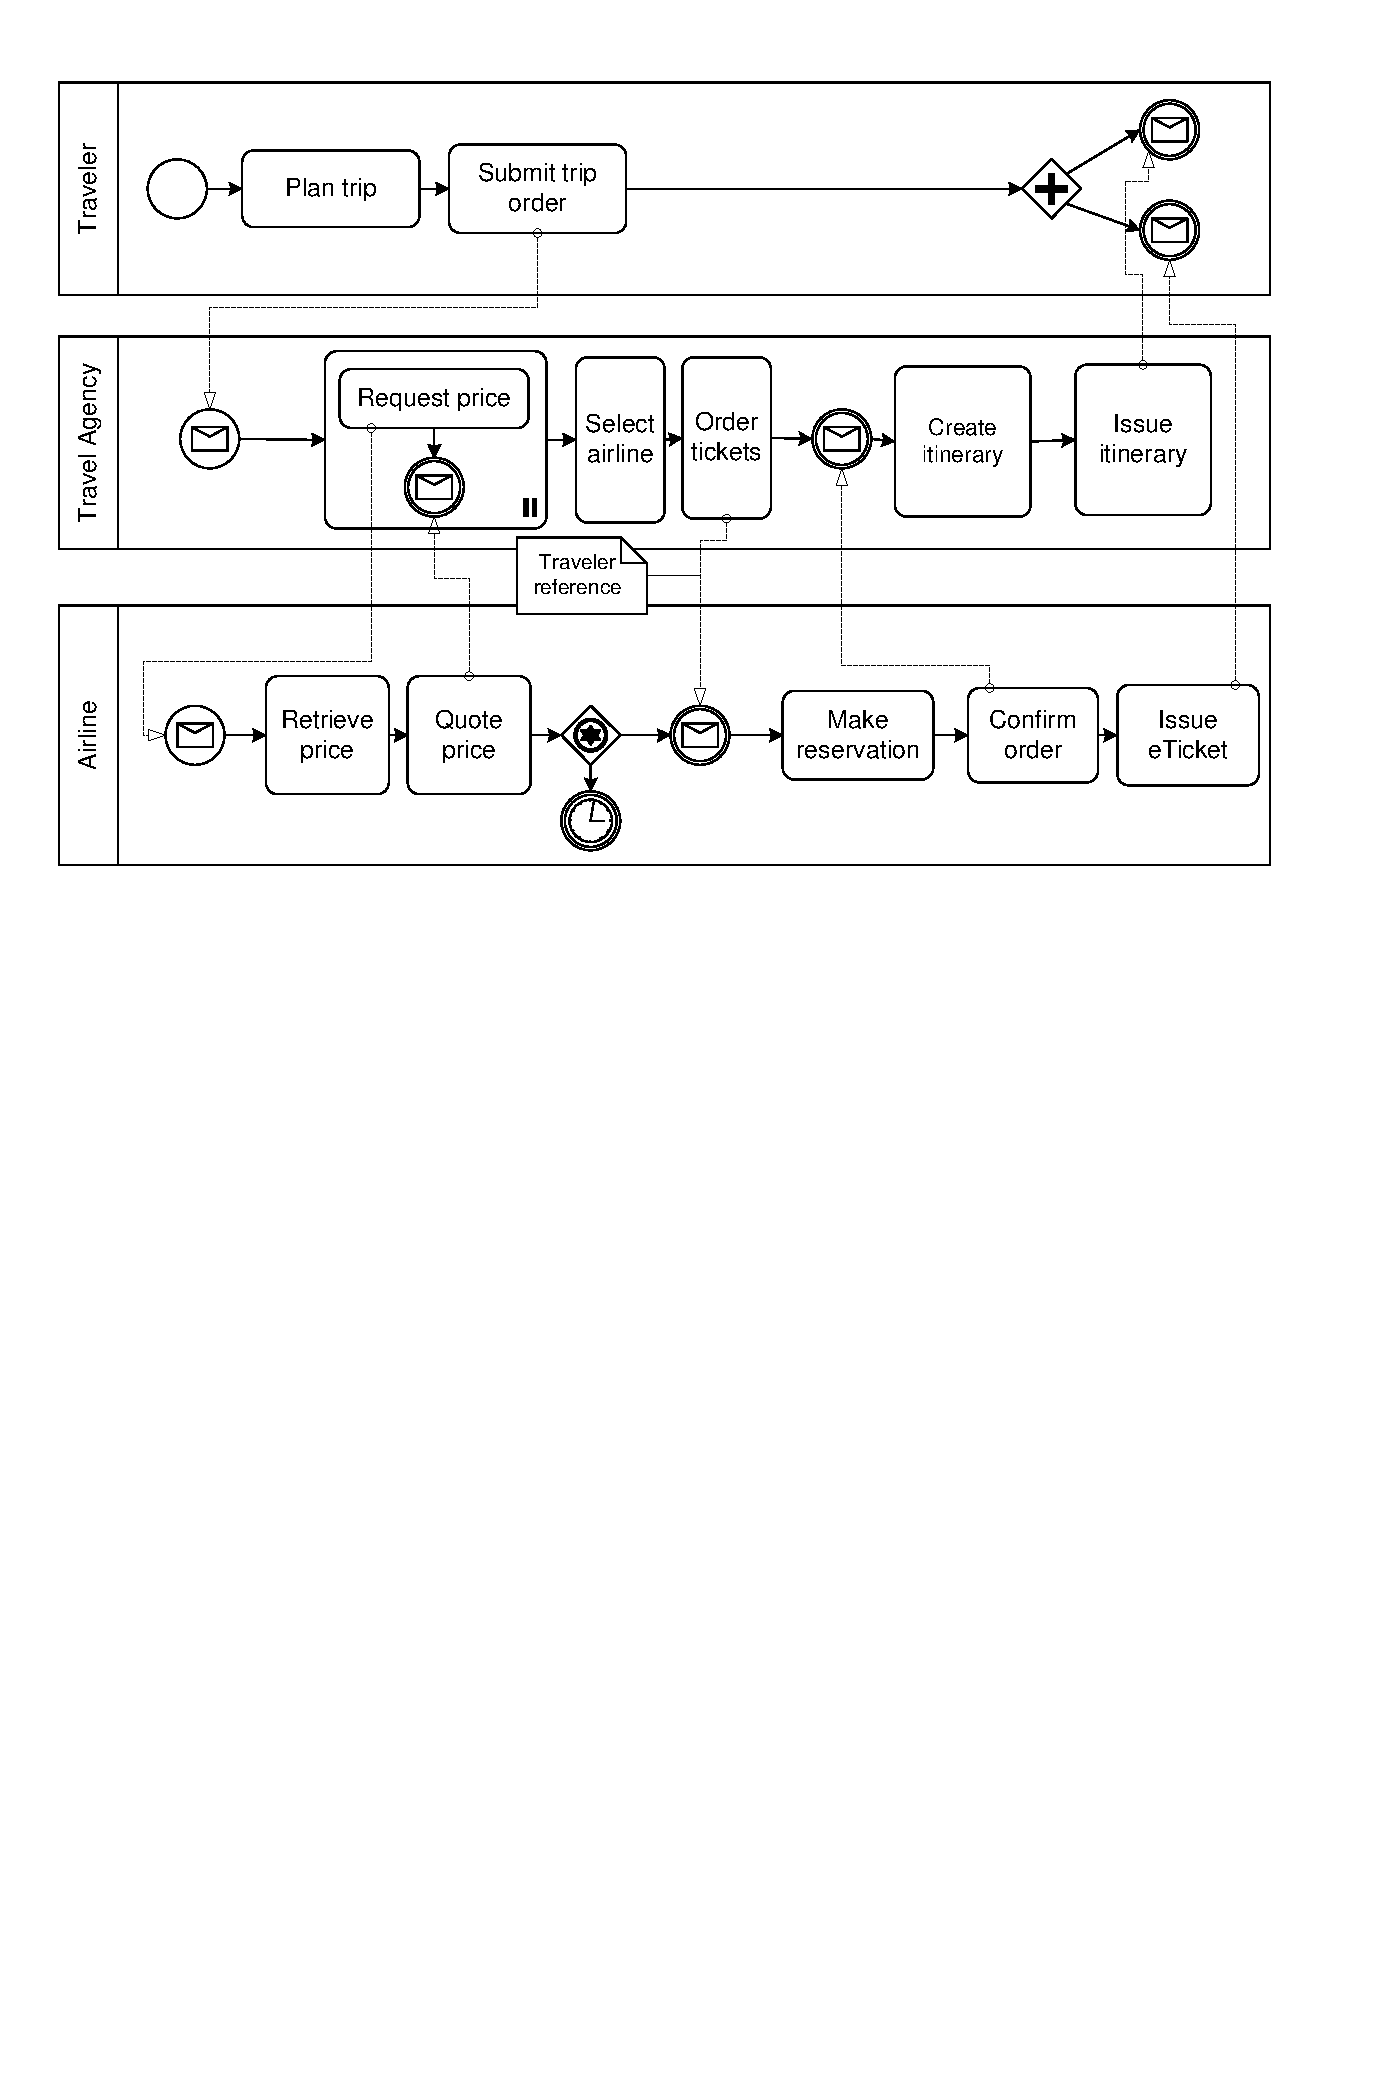
\includegraphics[width=\textwidth]{choreography.pdf}
  \caption{Example Choreography}
  \label{fig:chor1}
\end{figure}

\begin{figure}
  \centering
  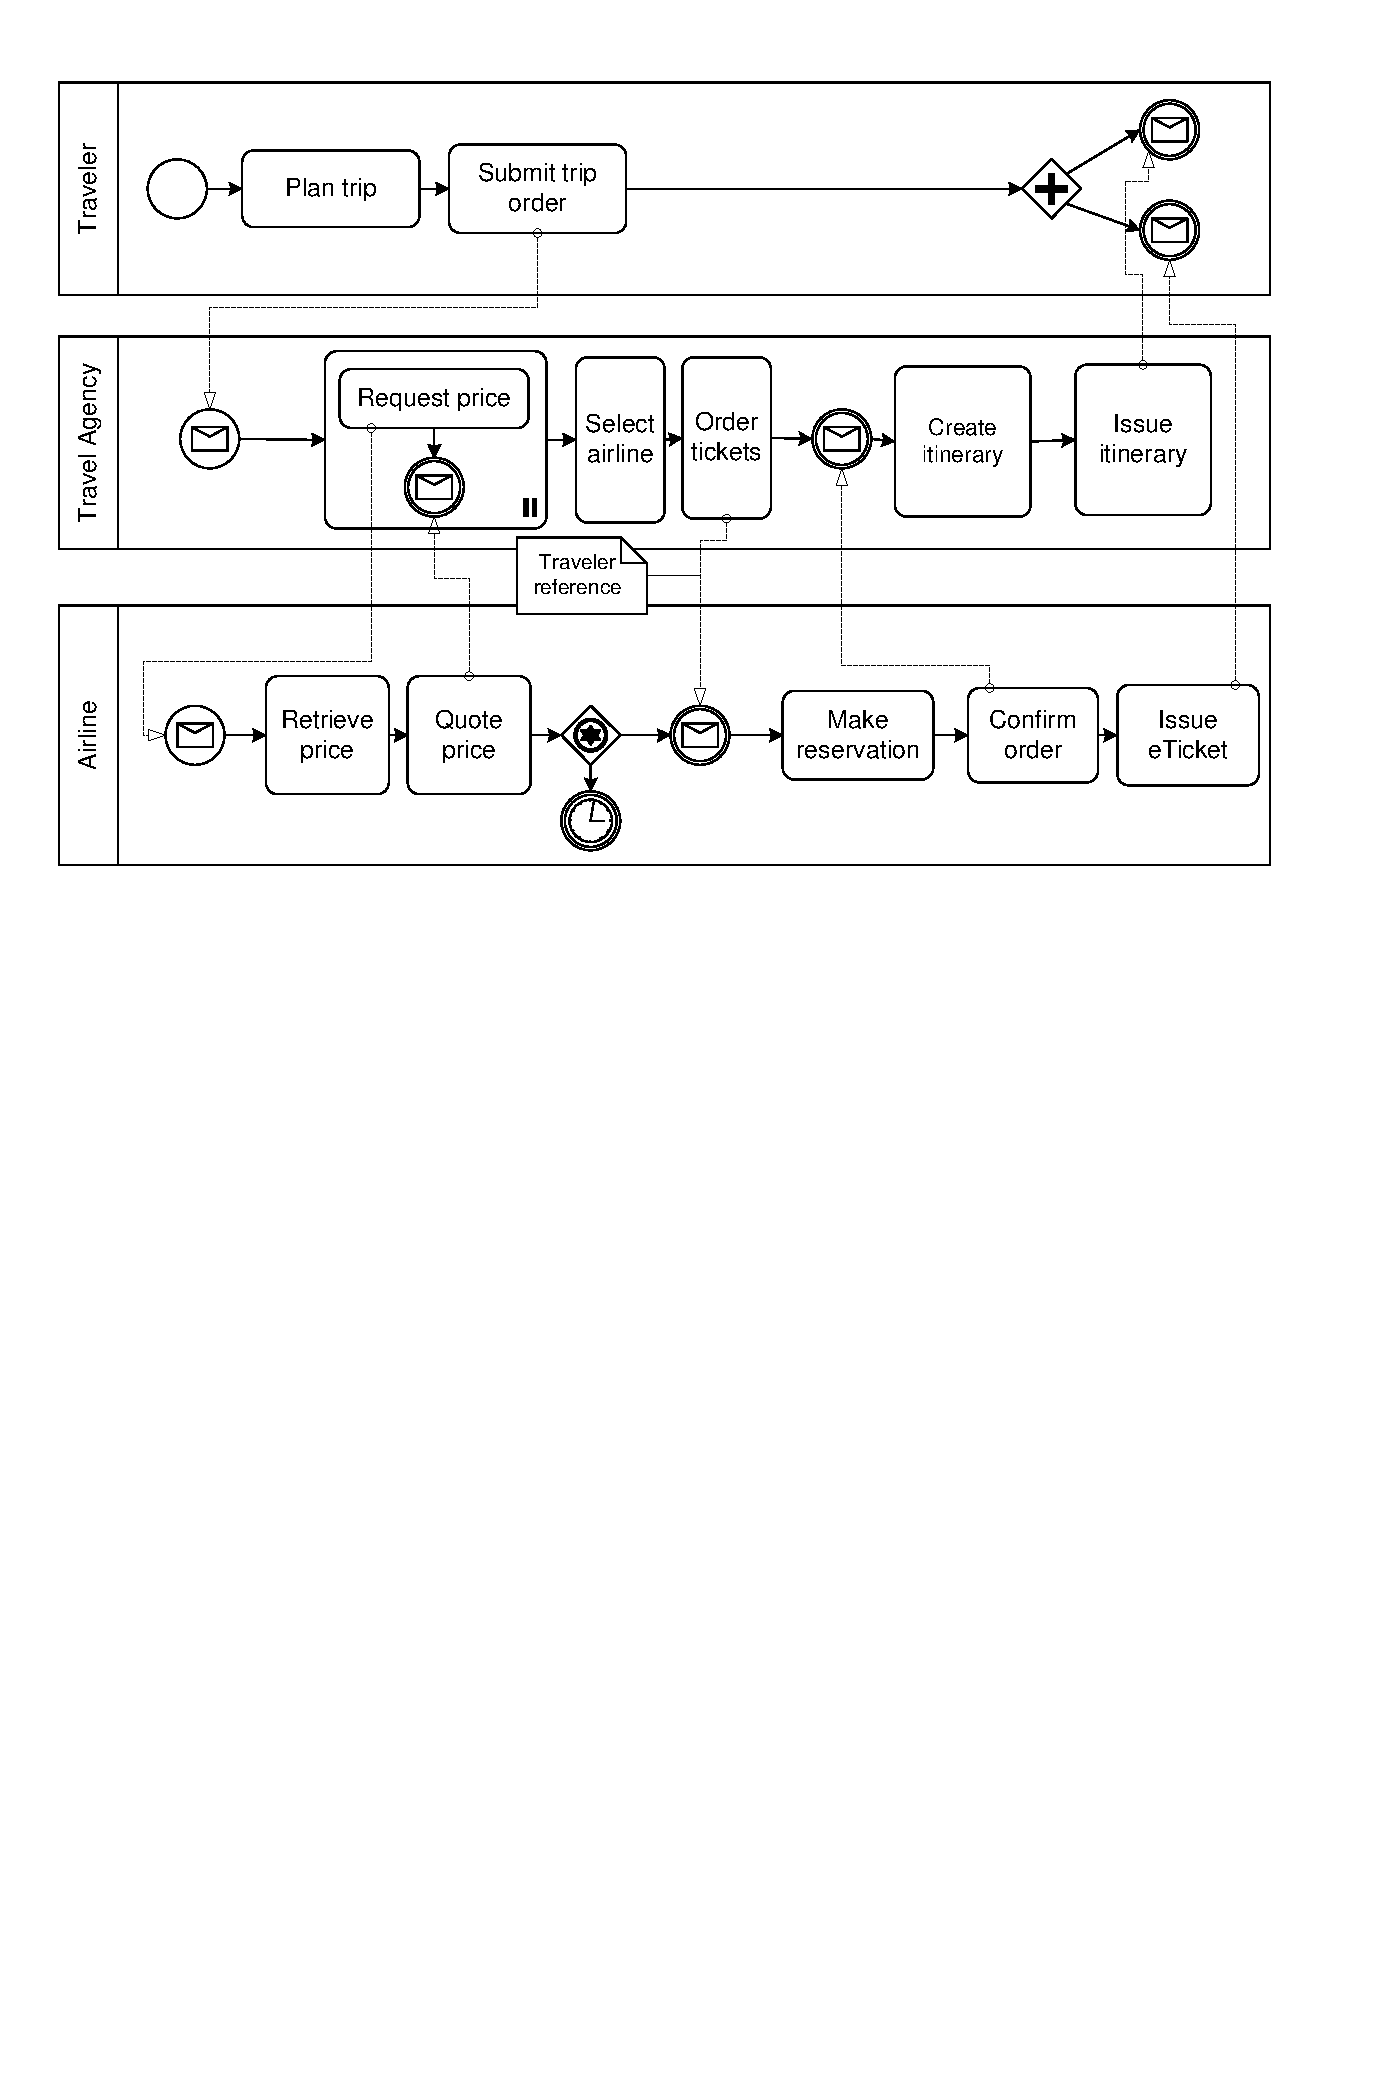
\includegraphics[width=.8\textwidth]{choreography.pdf}
  \caption[Example Choreography]{The example choreography. Now slightly smaller to demonstrate \texttt{\textbackslash textwidth}. And also the use of alternative captions for the list of images. However, the latter is only conditionally recommended, because who reads so much text under a picture? Or is it just a matter of style?}
  \label{fig:chor2}
\end{figure}


\begin{figure}
  \hfill
  \begin{subfigure}{.3\textwidth}
    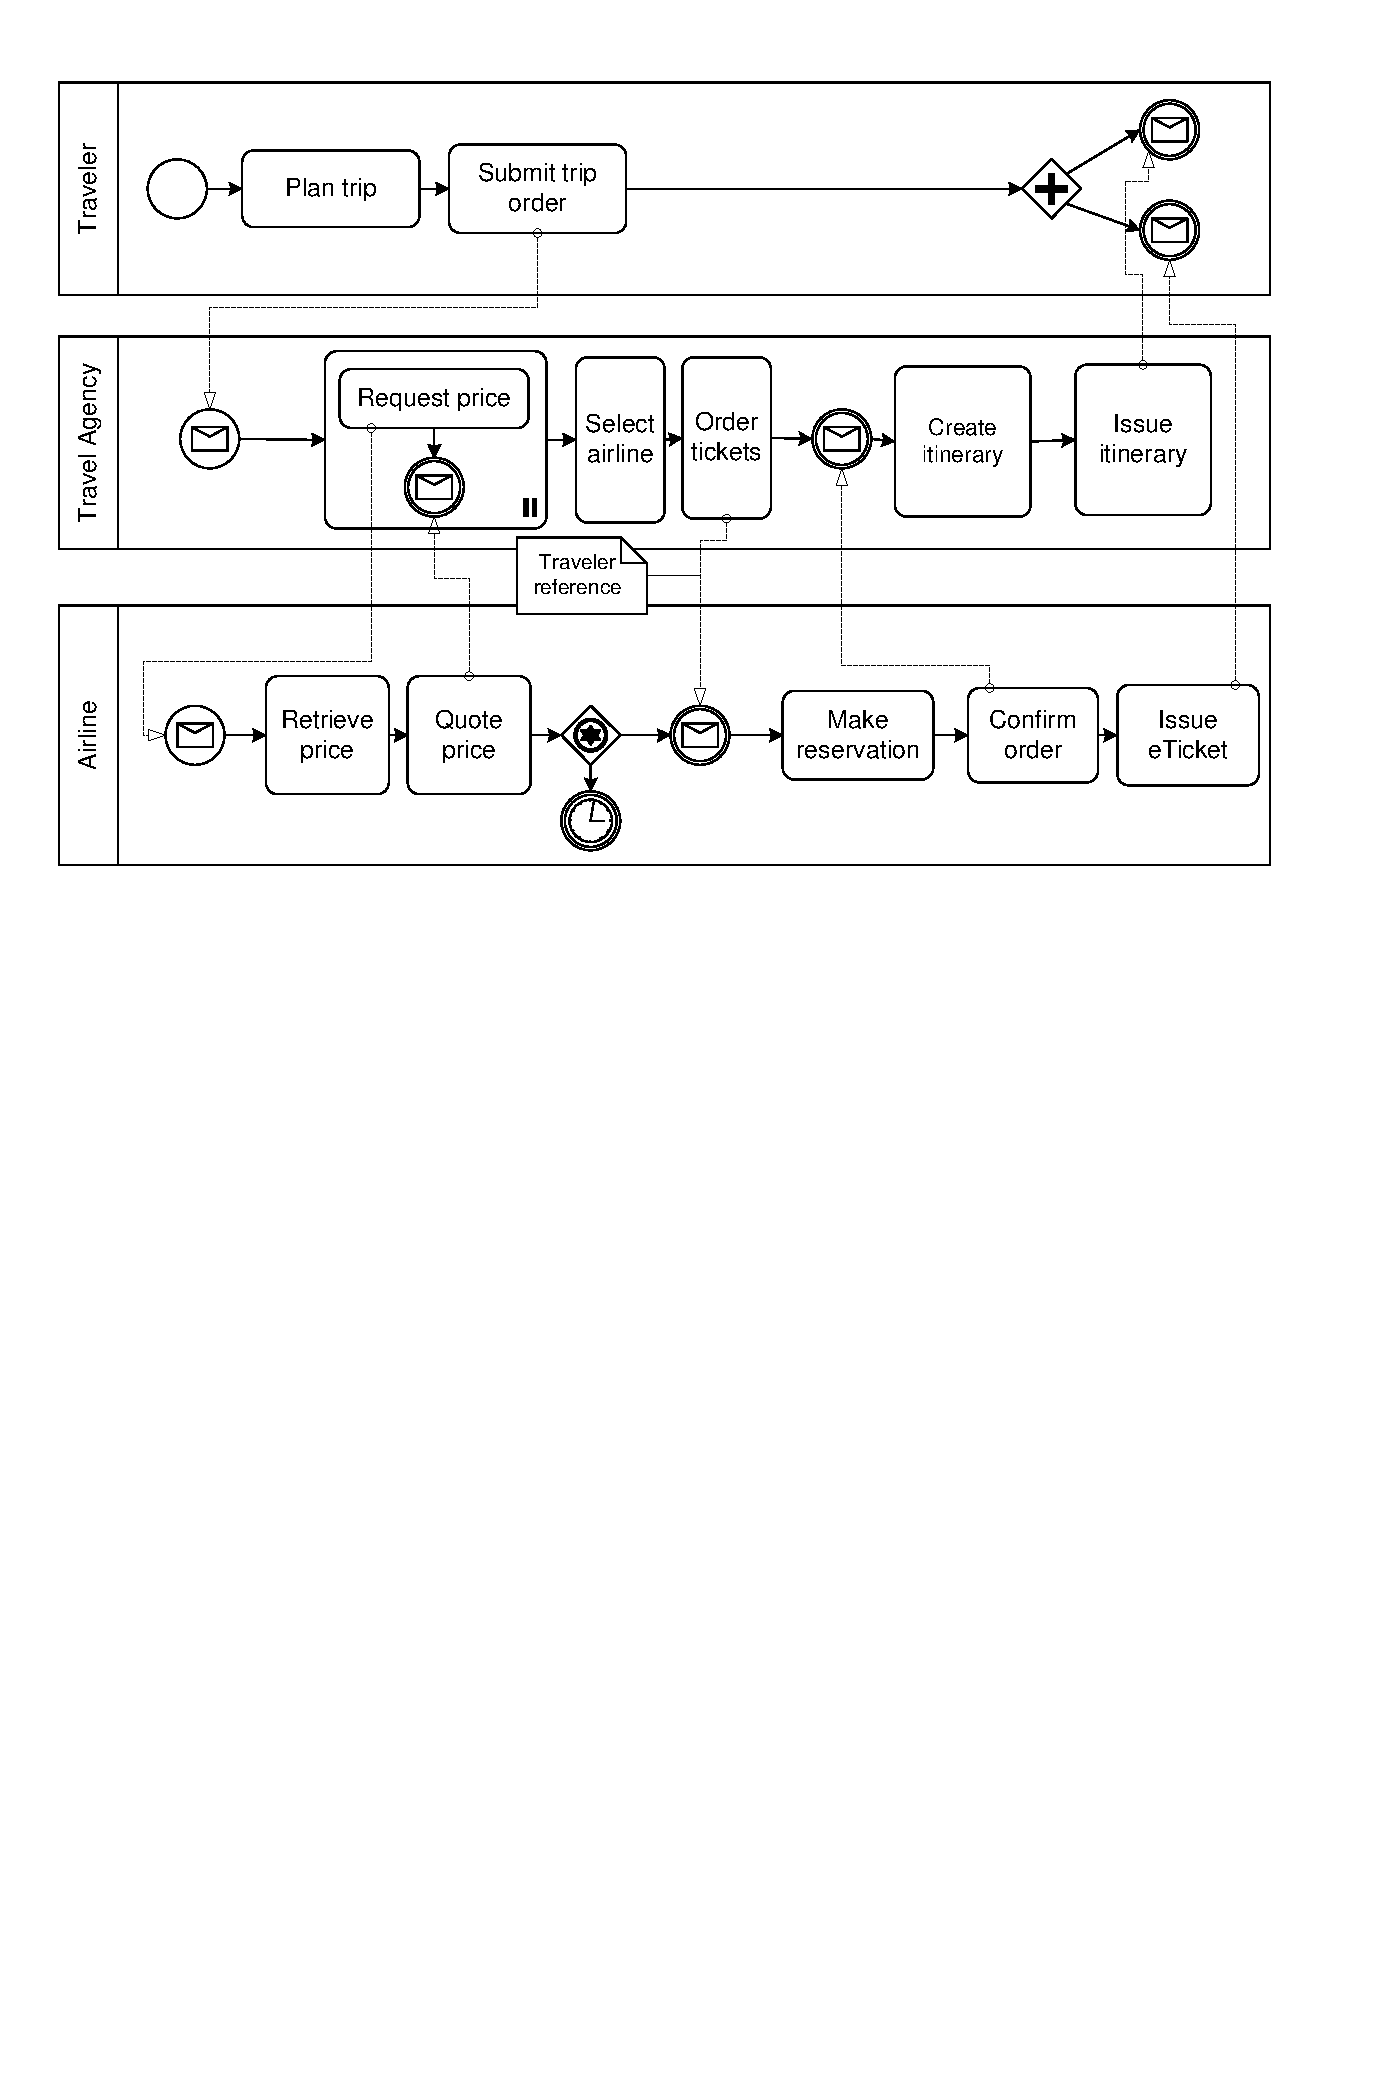
\includegraphics[width=\textwidth]{choreography.pdf}
    \caption{Choreography 1}
    \label{fig:subfigA}
  \end{subfigure}
  \hfill
  \begin{subfigure}{.3\textwidth}
    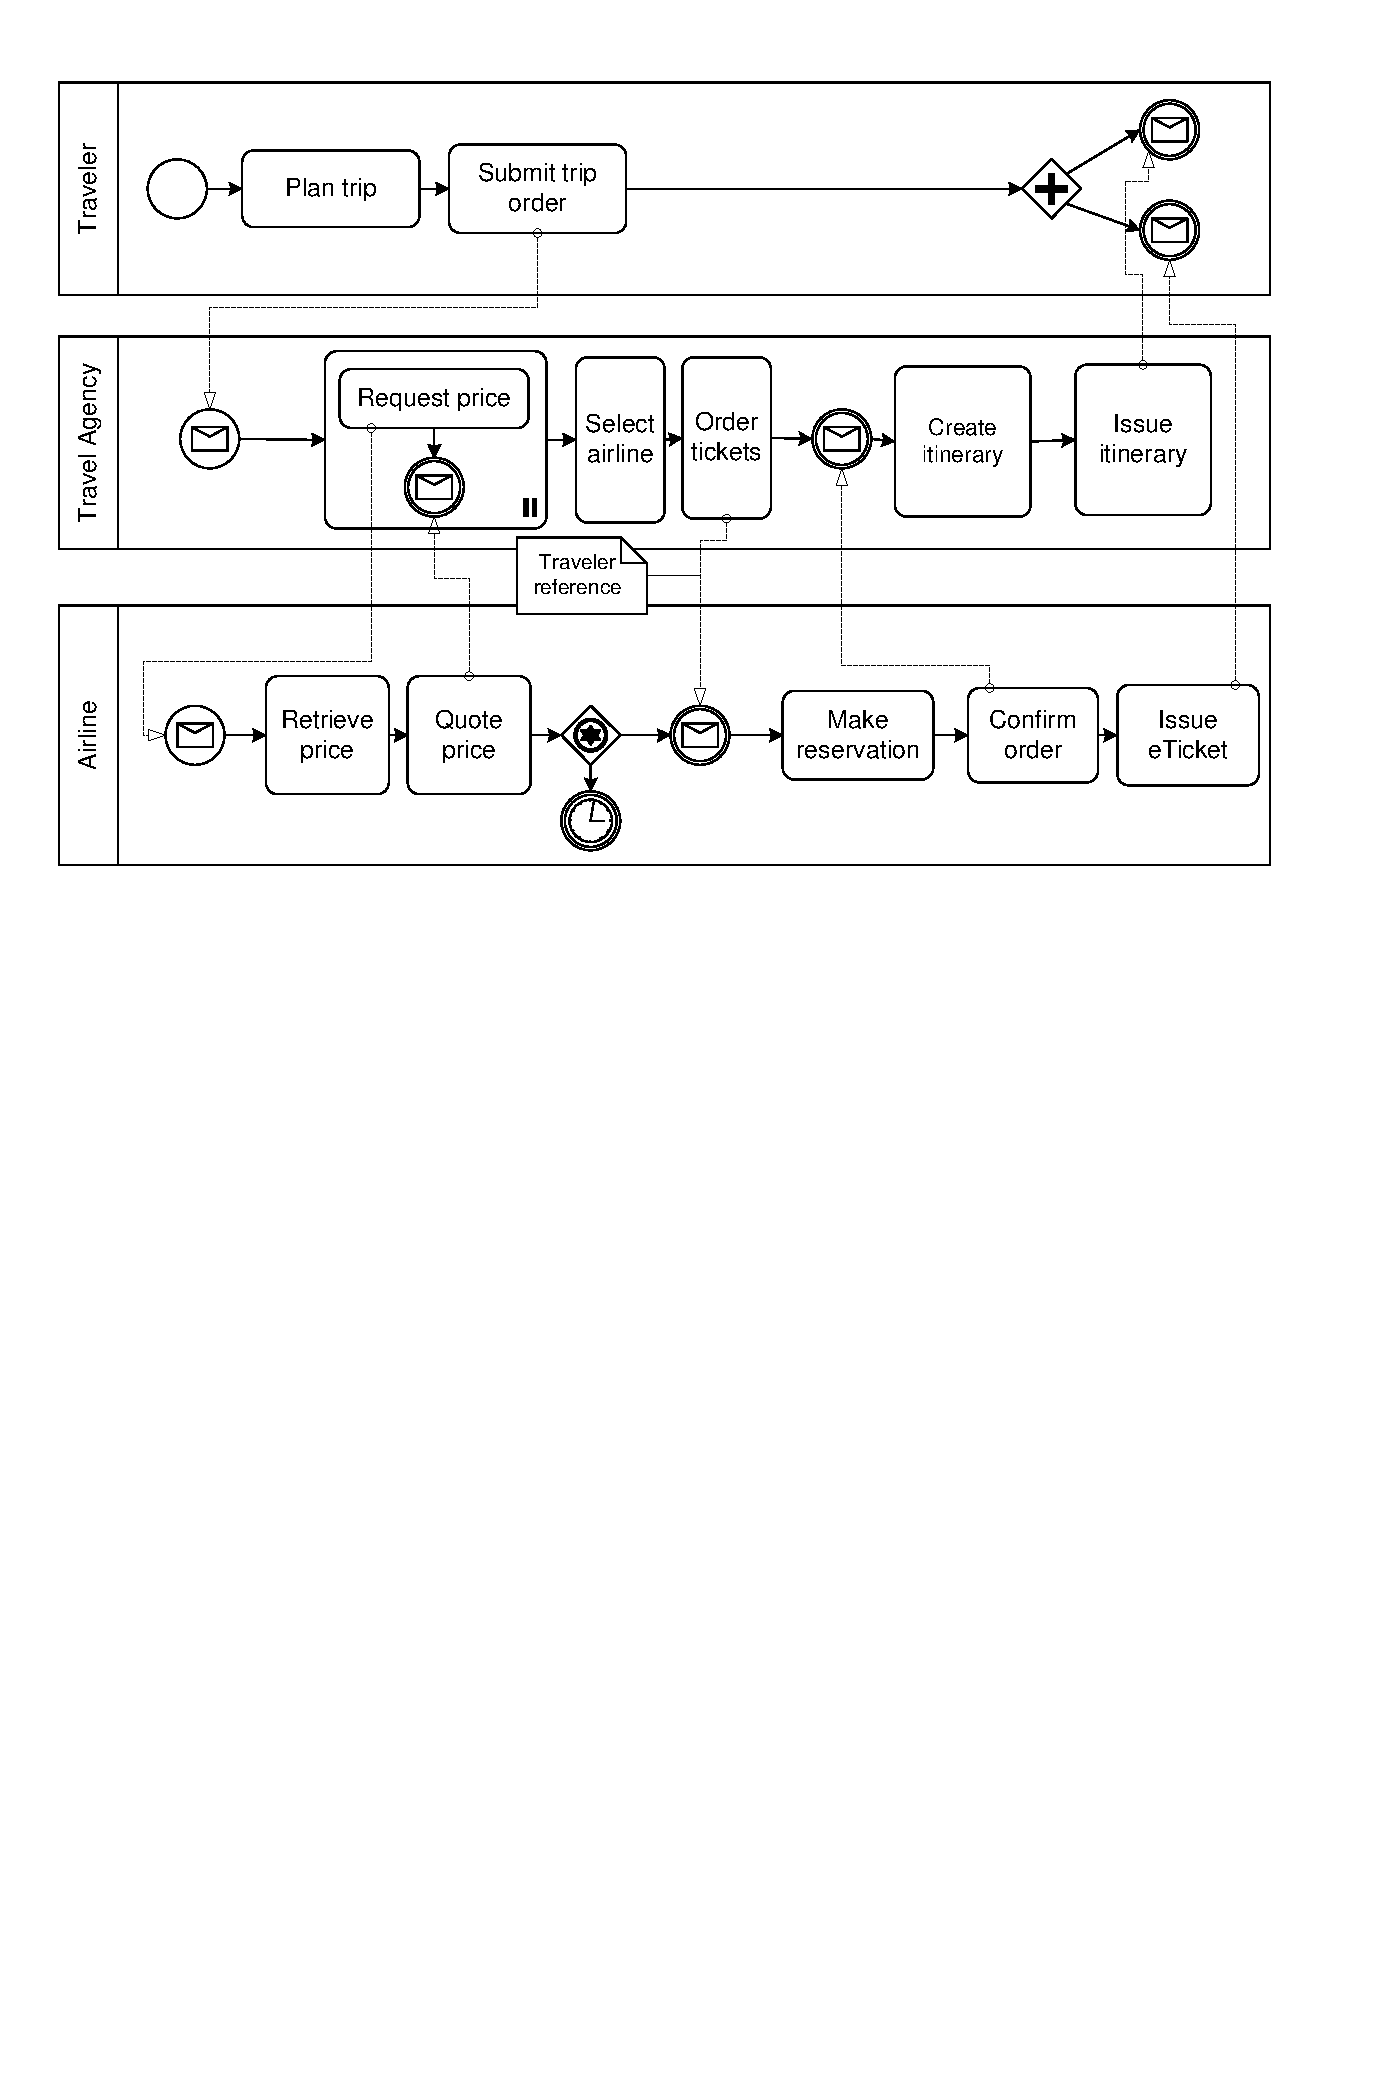
\includegraphics[width=\textwidth]{choreography.pdf}
    \caption{Choreography 2}
    \label{fig:subfigB}
  \end{subfigure}
  \hfill
  \begin{subfigure}{.3\textwidth}
    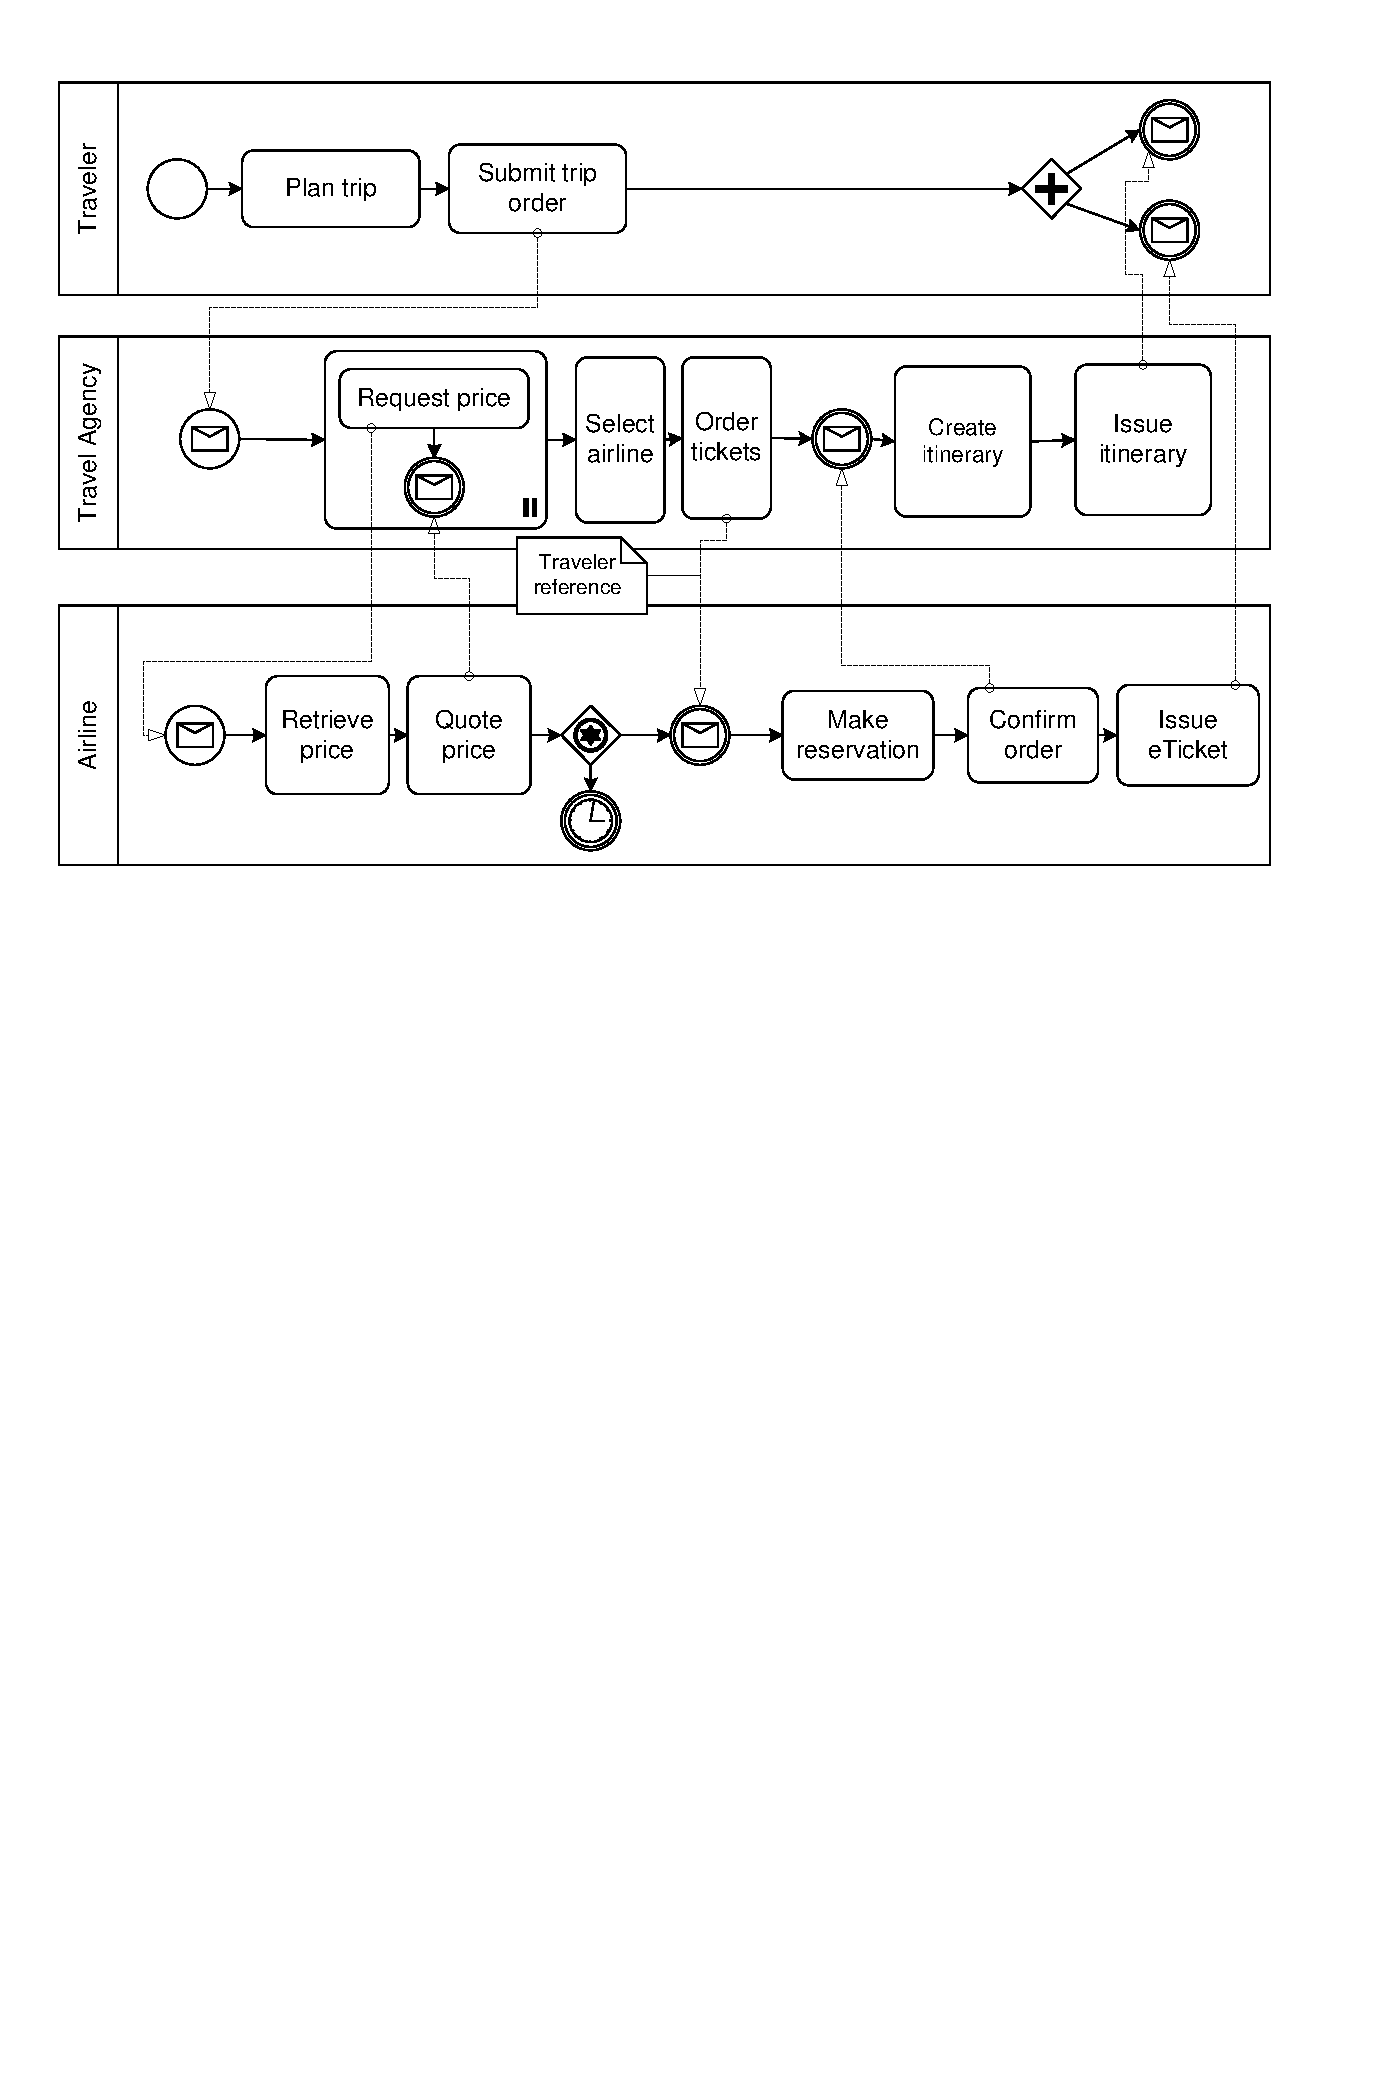
\includegraphics[width=.9\textwidth]{choreography.pdf}
    \caption{Choreography 3}
    \label{fig:subfigC}
  \end{subfigure}
  \caption{Example to place 3 illustrations next to each other. Further, it is possible to reference each separately.}
  \label{fig:subfig_example}
\end{figure}

\Cref{fig:subfig_example} shows the usage of the package subcaption.
It is indeed possible to reference to sub figures: \Cref{fig:subfigA}.

It is possible to convert SVGs to PDF directly during compilation.
This is described in the source code of latex-tipps.tex, but commented out.

\iffalse % <-- Take this away if inkscape is in the path
  The SVG in \cref{fig:directSVG} is directly included, while the text in the SVG in \cref{fig:latexSVG} is set using pdflatex.
  If you want to see the graphics, inkscape must be in PATH and in the text source \texttt{\textbackslash{}iffalse} and \text{\textbackslash{}iftrue} have to be commented out.

  \begin{figure}
    \centering
    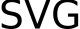
\includegraphics{svgexample.svg}
    \caption{SVG directly included}
    \label{fig:directSVG}
  \end{figure}

  \begin{figure}
    \centering
    \def\svgwidth{.4\textwidth}
    \includesvg{svgexample}
    \caption{Text in SVN set via \LaTeX{}}
    \label{fig:latexSVG}
  \end{figure}
\fi % <-- Take this away if inkscape is in the path



\section{More Illustrations}
\Cref{fig:AnhangsChor,fig:AnhangsChor2} show two choreographies, which should further explain the facts. The second figure is rotated 90 degrees to demonstrate the \texttt{pdflscape} package.

\begin{figure}
  \centering
  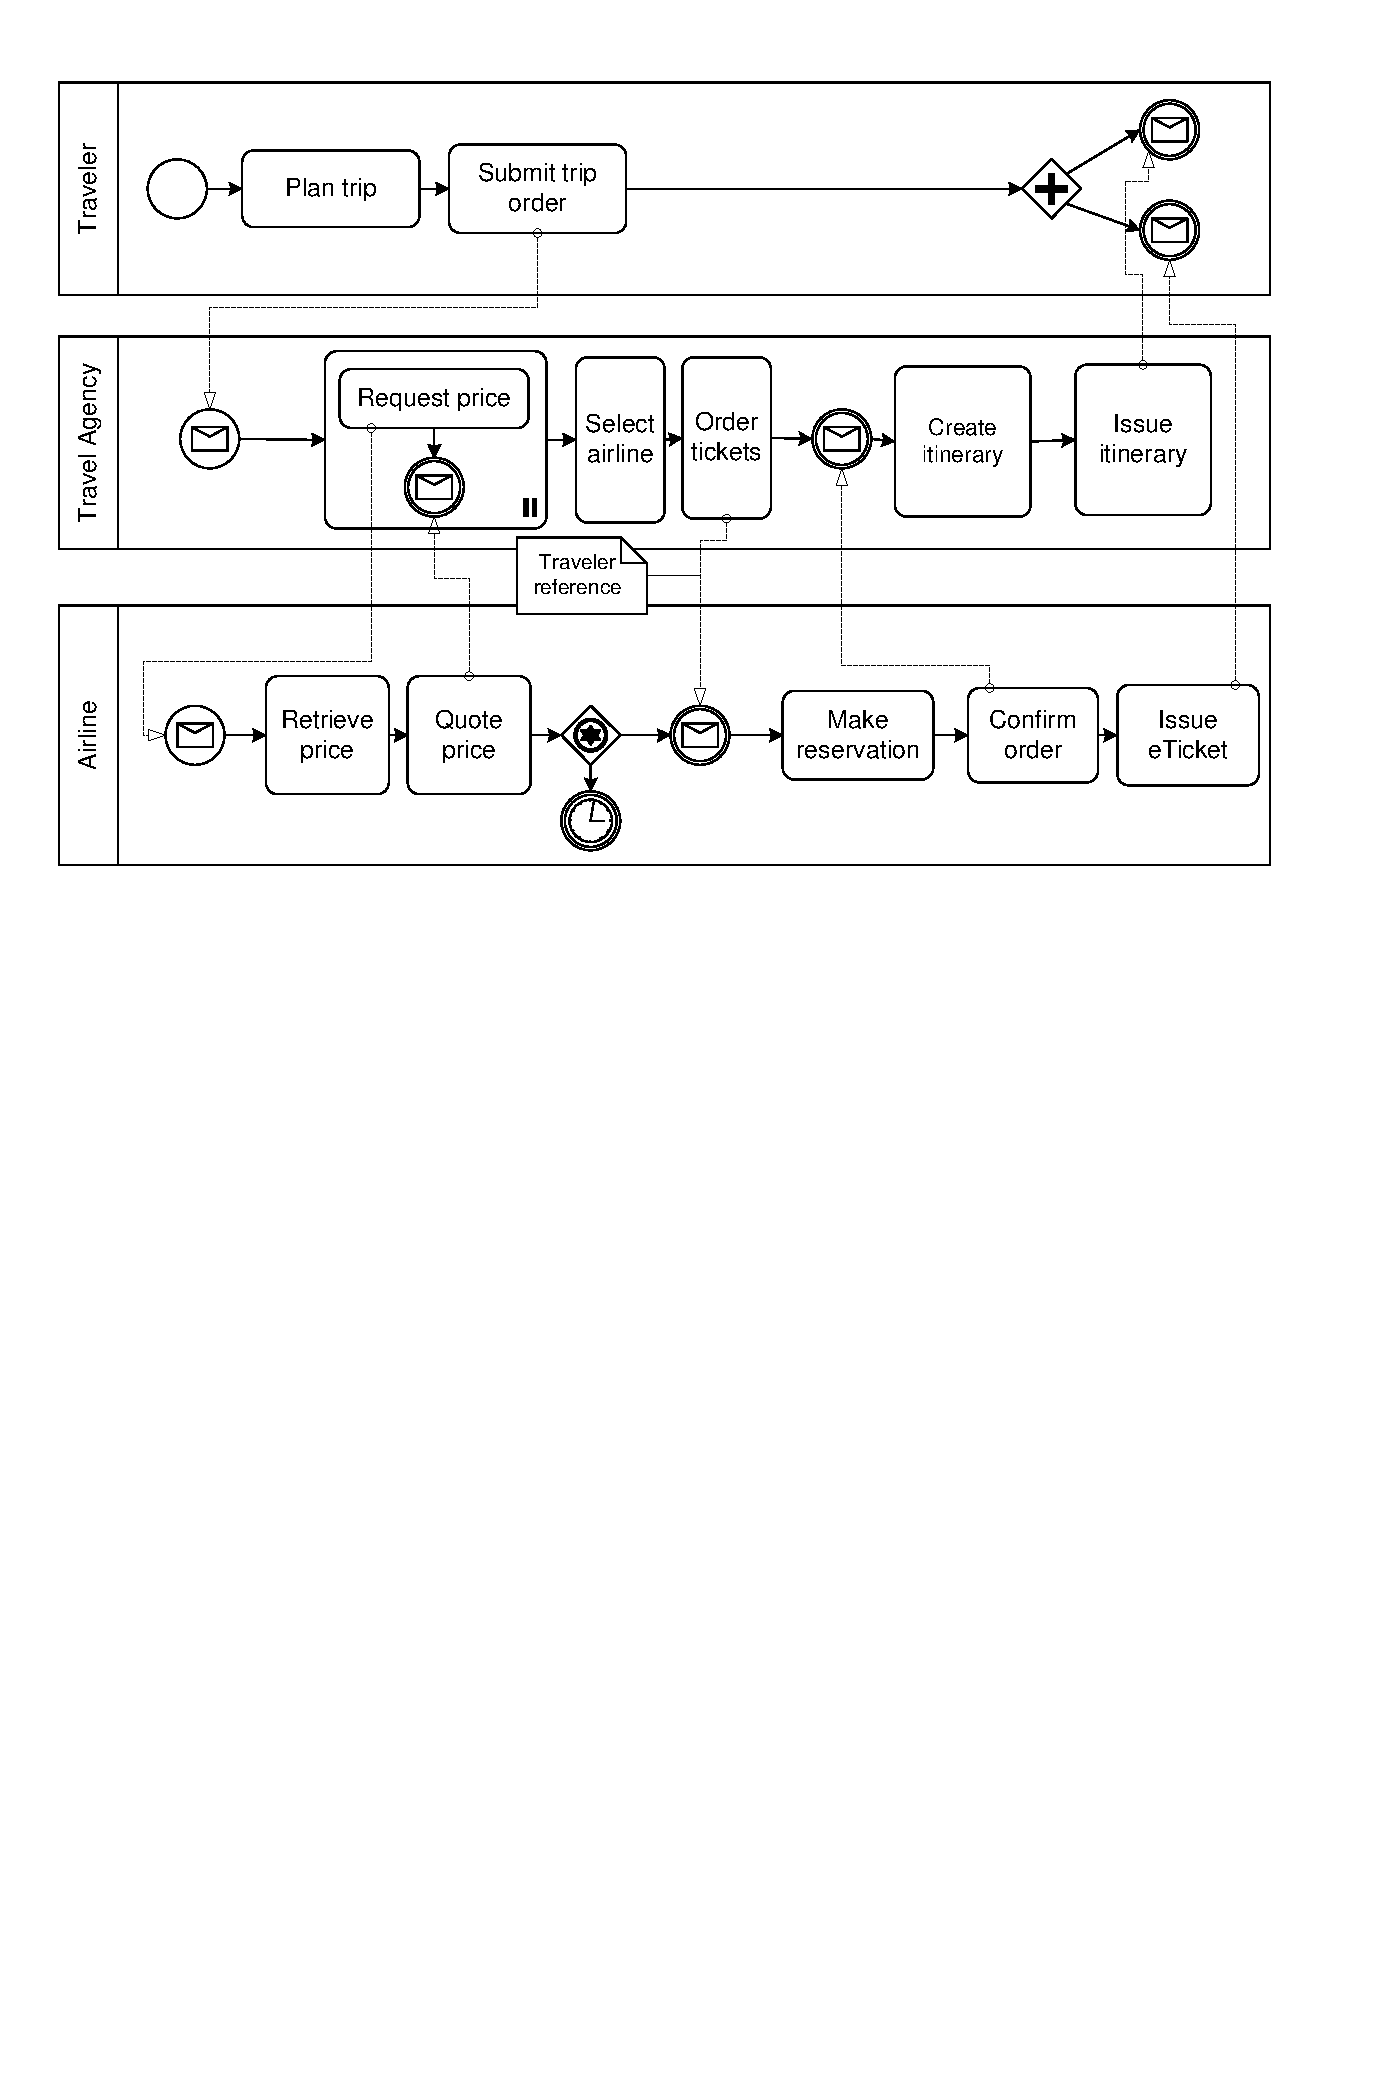
\includegraphics[width=\textwidth]{choreography.pdf}
  \caption{Example Choreography I}
  \label{fig:AnhangsChor}
\end{figure}

\begin{landscape}
  %sidewaysfigure
  \begin{figure}
    \centering
    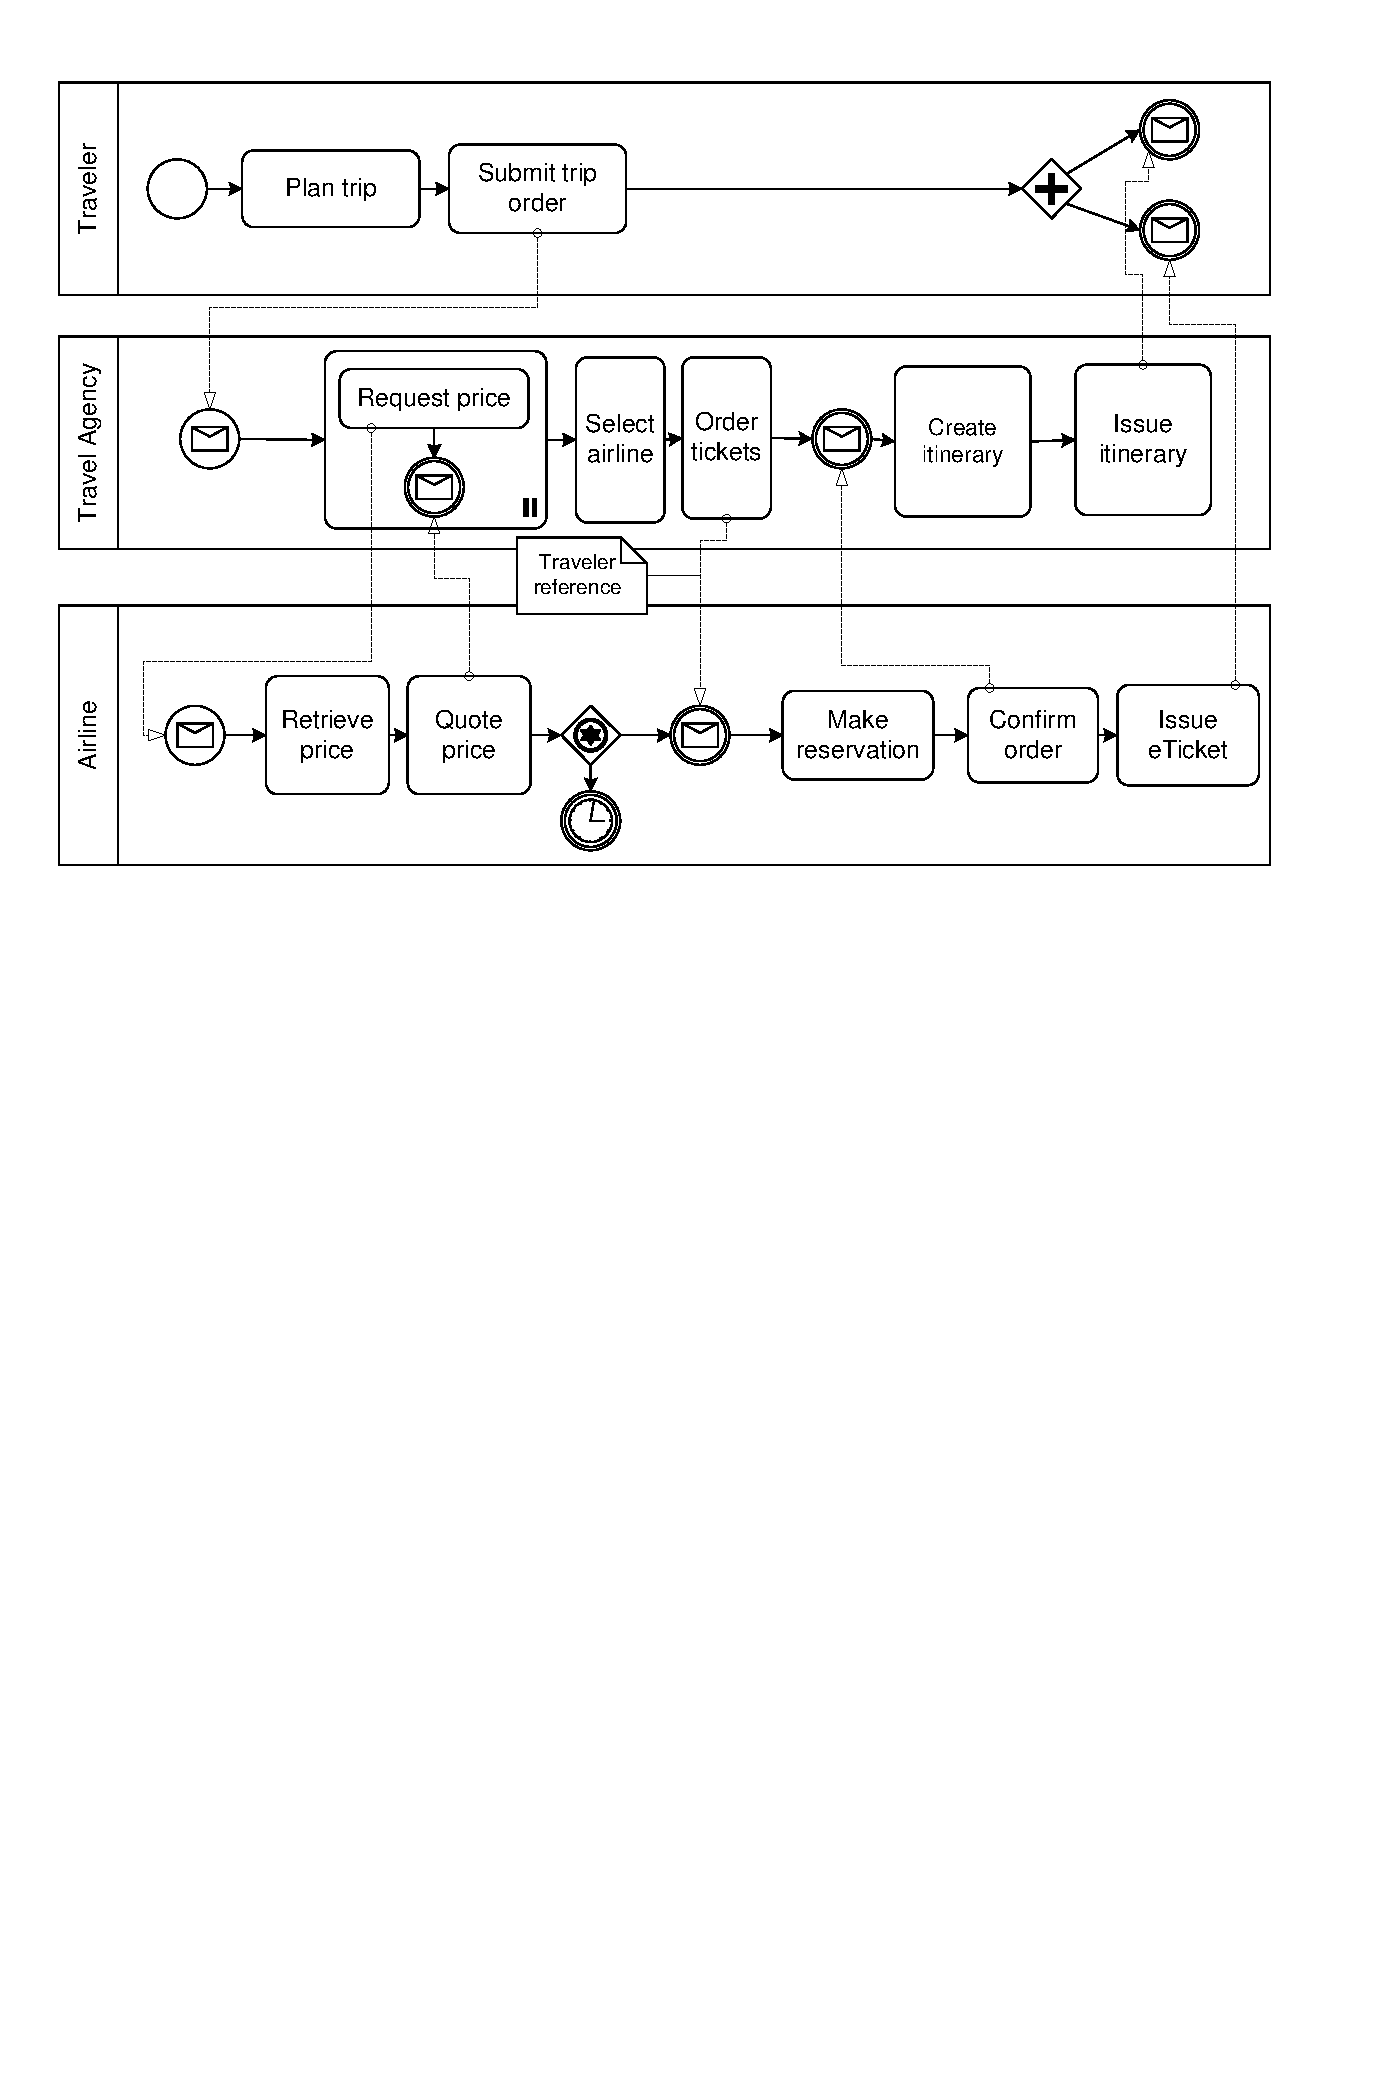
\includegraphics[width=\textwidth]{choreography.pdf}
    \caption{Example Choreography II}
    \label{fig:AnhangsChor2}
  \end{figure}
\end{landscape}


\IfFileExists{pgfplots.sty}{
  %%%%%%%%%%%%%%%%%%%%%%%%%%%%%%%%%%%%%%%%%%%%%%%%%%%%%%%%%%%%%%%%%%%%%%%%%%%%%%
  \section{Plots with pgfplots}
  %%%%%%%%%%%%%%%%%%%%%%%%%%%%%%%%%%%%%%%%%%%%%%%%%%%%%%%%%%%%%%%%%%%%%%%%%%%%%%
  The package pdfplots provides plotting of functions directly in \LaTeX~like with matlab or gnuplot. Some visual examples are available here\footnote{\url{http://texdoc.net/pkg/visualtikz}}.
  \begin{figure}[h]
    \centering
    \begin{tikzpicture}
      \begin{axis}[xlabel=$x$,
          ylabel=$\sin(x)$]
        \addplot {sin(deg(x))};  % Print sine function
      \end{axis}
    \end{tikzpicture}
    \caption{Plot of $\sin(x)$ direclty inside the figure environment with pgfplots.}
  \end{figure}

  \begin{figure}[h]
    \centering
    \begin{tikzpicture}
      \begin{axis}[xlabel=$x$,
          ylabel=$y$]
        \addplot table [x=a, y=c, col sep=comma] {data/data.csv};  % Read coordinates from csv file and plot them
      \end{axis}
    \end{tikzpicture}
    \caption{Coordinates $x$ and $y$ read from csv file and plotted pgfplots.}
  \end{figure}

}{}


%%%%%%%%%%%%%%%%%%%%%%%%%%%%%%%%%%%%%%%%%%%%%%%%%%%%%%%%%%%%%%%%%%%%%%%%%%%%%%
\section{Figures with tikz}
%%%%%%%%%%%%%%%%%%%%%%%%%%%%%%%%%%%%%%%%%%%%%%%%%%%%%%%%%%%%%%%%%%%%%%%%%%%%%%
The tikz is a package for creating graphics programmatically. With this package grids or other regular strucutres can be easliy generated.

\begin{figure}[ht]
  \centering
  \begin{tikzpicture}
    \draw(0,0) rectangle (4,4);
    \foreach \x in {0.5,1,1.5,2,2.5,3,3.5}
    \foreach \y in {0.5,1,1.5,2,2.5,3,3.5}
    \draw(\x,\y) circle (1pt);
  \end{tikzpicture}
  \caption{A regular grid genrated with easily with two for loops.}\label{fig:tikz_example}
\end{figure}


%%%%%%%%%%%%%%%%%%%%%%%%%%%%%%%%%%%%%%%%%%%%%%%%%%%%%%%%%%%%%%%%%%%%%%%%%%%%%%
\section{UML diagrams using tikz-uml}
%%%%%%%%%%%%%%%%%%%%%%%%%%%%%%%%%%%%%%%%%%%%%%%%%%%%%%%%%%%%%%%%%%%%%%%%%%%%%%

\Cref{fig:uml} presents a class diagram typeset using tikz-uml.

\begin{figure}
  \centering
  \begin{tikzpicture}
  \begin{umlpackage}{p}
  \begin{umlpackage}{sp1}
  \umlclass[template=T]{A}{
    n : uint \\ t : float
  }{}
  \umlclass[y=-3]{B}{
    d : double
  }{
    \umlvirt{setB(b : B) : void} \\ getB() : B}
  \end{umlpackage}
  \begin{umlpackage}[x=10,y=-6]{sp2}
  \umlinterface{C}{
    n : uint \\ s : string
  }{}
  \end{umlpackage}
  \umlclass[x=2,y=-10]{D}{
    n : uint
    }{}
  \end{umlpackage}

  \umlassoc[geometry=-|-, arg1=tata, mult1=*, pos1=0.3, arg2=toto, mult2=1, pos2=2.9, align2=left]{C}{B}
  \umlunicompo[geometry=-|, arg=titi, mult=*, pos=1.7, stereo=vector]{D}{C}
  \umlimport[geometry=|-, anchors=90 and 50, name=import]{sp2}{sp1}
  \umlaggreg[arg=tutu, mult=1, pos=0.8, angle1=30, angle2=60, loopsize=2cm]{D}{D}
  \umlinherit[geometry=-|]{D}{B}
  \umlnote[x=2.5,y=-6, width=3cm]{B}{A note with respect to class B}
  \umlnote[x=7.5,y=-2]{import-2}{A anotation}
  \end{tikzpicture}
  \caption{Class diagram generated with tikz-uml. Example adapted from Nicolas Kielbasiewicz.}
  \label{fig:uml}
\end{figure}

\section{UML diagrams using PlantUML}

In case \lualatex{} is used and PlantUML is installed, UML diagrams can be defined using PlantUML.

% Only works if "--shell-escape" is activated. Please activate only if you are sure, your compilation settings are correct
%\IfFileExists{plantuml.sty}{\input{latexhints-english-plantuml}}{}


%%%%%%%%%%%%%%%%%%%%%%%%%%%%%%%%%%%%%%%%%%%%%%%%%%%%%%%%%%%%%%%%%%%%%%%%%%%%%%
\section{Linguistic Forests}
%%%%%%%%%%%%%%%%%%%%%%%%%%%%%%%%%%%%%%%%%%%%%%%%%%%%%%%%%%%%%%%%%%%%%%%%%%%%%%

\begin{filecontents*}{\democodefile}
\begin{forest}
  [VP
    [DP]
    [V’
      [V]
      [DP]
    ]
  ]
\end{forest}
\end{filecontents*}
\PrintDemo{style=parallel}


%%%%%%%%%%%%%%%%%%%%%%%%%%%%%%%%%%%%%%%%%%%%%%%%%%%%%%%%%%%%%%%%%%%%%%%%%%%%%%
\section{Tables}
%%%%%%%%%%%%%%%%%%%%%%%%%%%%%%%%%%%%%%%%%%%%%%%%%%%%%%%%%%%%%%%%%%%%%%%%%%%%%%
\cref{tab:Ergebnisse} shows results and \cref{tab:Werte} shows how numerical data can be represented in a table.
\begin{table}
  \centering
  \begin{tabular}{ccc}
    \toprule
    \multicolumn{2}{c}{\textbf{summed}} & \textbf{Title}                                                          \\ \midrule
    Table                                      & as                                                           & in      \\
    \url{tabsatz.pdf}                            & recommended                                                     & gesetzt \\

    \multirow{2}{*}{Example}                    & \multicolumn{2}{c}{a nice example}                                \\
                                                 & \multicolumn{2}{c}{for using \qq{multirow}}           \\
    \bottomrule
  \end{tabular}
  \caption[Example Table]{Exampe Table -- see \url{http://www.ctan.org/tex-archive/info/german/tabsatz/}}
  \label{tab:Ergebnisse}
\end{table}

\begin{table}
  \centering
  \begin{tabular}{l *{8}{d{3.2}}}
    \toprule

                         & \multicolumn{2}{c}{\textbf{Parameter 1}} & \multicolumn{2}{c}{\textbf{Parameter 2}} & \multicolumn{2}{c}{\textbf{Parameter 3}} & \multicolumn{2}{c}{\textbf{Parameter 4}}                                                                                                                                       \\
    \cmidrule(r){2-3}\cmidrule(lr){4-5}\cmidrule(lr){6-7}\cmidrule(l){8-9}

    \textbf{Bedingungen} & \multicolumn{1}{c}{\textbf{M}}           & \multicolumn{1}{c}{\textbf{SD}}          & \multicolumn{1}{c}{\textbf{M}}           & \multicolumn{1}{c}{\textbf{SD}}          & \multicolumn{1}{c}{\textbf{M}} & \multicolumn{1}{c}{\textbf{SD}} & \multicolumn{1}{c}{\textbf{M}} & \multicolumn{1}{c}{\textbf{SD}} \\
    \midrule

    W                    & 1.1                                      & 5.55                                     & 6.66                                     & .01                                      &                                &                                 &                                &                                 \\
    X                    & 22.22                                    & 0.0                                      & 77.5                                     & .1                                       &                                &                                 &                                &                                 \\
    Y                    & 333.3                                    & .1                                       & 11.11                                    & .05                                      &                                &                                 &                                &                                 \\
    Z                    & 4444.44                                  & 77.77                                    & 14.06                                    & .3                                       &                                &                                 &                                &                                 \\
    \bottomrule
  \end{tabular}

  \caption{Example table for 4 constraints (W-Z), each having 4 parameters with (M und SD). Note: use always the same number of decimal places.}
  \label{tab:Werte}
\end{table}

\IfFileExists{pgfplotstable.sty}{

\subsection{Tables with pgfplots}
With the pgfplotstable package tables can be directly generated from a csv file.

\begin{table}[h]
\centering
\pgfplotstabletypeset[
col sep = comma,
every head row/.style={before row=\toprule,after row=\midrule},
every last row/.style={after row=\bottomrule},
display columns/0/.style={string type,column name={}}
]
{data/data.csv}
\caption{Table direclty generated from the values of a csf file.}
\end{table}
}{}


\section{Tables spanning multiple pages}


\begin{longtable}{|l|l|l|}
\caption{A sample long table.} \label{tab:long} \\

\hline \multicolumn{1}{|c|}{\textbf{First column}} & \multicolumn{1}{c|}{\textbf{Second column}} & \multicolumn{1}{c|}{\textbf{Third column}} \\ \hline
\endfirsthead

\multicolumn{3}{c}%
{{\bfseries \tablename\ \thetable{} -- continued from previous page}} \\
\hline \multicolumn{1}{|c|}{\textbf{First column}} & \multicolumn{1}{c|}{\textbf{Second column}} & \multicolumn{1}{c|}{\textbf{Third column}} \\ \hline
\endhead

\hline \multicolumn{3}{|r|}{{Continued on next page}} \\ \hline
\endfoot

\hline \hline
\endlastfoot

A & BC & D \\
A & BC & D \\
A & BC & D \\
A & BC & D \\
A & BC & D \\
A & BC & D \\
A & BC & D \\
A & BC & D \\
A & BC & D \\
A & BC & D \\
A & BC & D \\
A & BC & D \\
A & BC & D \\
A & BC & D \\
A & BC & D \\
A & BC & D \\
A & BC & D \\
A & BC & D \\
A & BC & D \\
A & BC & D \\
A & BC & D \\
A & BC & D \\
A & BC & D \\
A & BC & D \\
A & BC & D \\
A & BC & D \\
A & BC & D \\
A & BC & D \\
A & BC & D \\
A & BC & D \\
A & BC & D \\
A & BC & D \\
A & BC & D \\
A & BC & D \\
A & BC & D \\
A & BC & D \\
A & BC & D \\
A & BC & D \\
A & BC & D \\
A & BC & D \\
A & BC & D \\
A & BC & D \\
A & BC & D \\
A & BC & D \\
A & BC & D \\
A & BC & D \\
A & BC & D \\
A & BC & D \\
A & BC & D \\
A & BC & D \\
A & BC & D \\
A & BC & D \\
A & BC & D \\
A & BC & D \\
A & BC & D \\
A & BC & D \\
A & BC & D \\
A & BC & D \\
A & BC & D \\
A & BC & D \\
A & BC & D \\
A & BC & D \\
A & BC & D \\
A & BC & D \\
A & BC & D \\
A & BC & D \\
A & BC & D \\
A & BC & D \\
A & BC & D \\
A & BC & D \\
A & BC & D \\
A & BC & D \\
A & BC & D \\
A & BC & D \\
A & BC & D \\
A & BC & D \\
A & BC & D \\
A & BC & D \\
A & BC & D \\
A & BC & D \\
\end{longtable}


%%%%%%%%%%%%%%%%%%%%%%%%%%%%%%%%%%%%%%%%%%%%%%%%%%%%%%%%%%%%%%%%%%%%%%%%%%%%%%
\section{Abbreviations}
%%%%%%%%%%%%%%%%%%%%%%%%%%%%%%%%%%%%%%%%%%%%%%%%%%%%%%%%%%%%%%%%%%%%%%%%%%%%%%
At the first pass the \gls{fr} was 5.
At the second pass was \gls{fr} 3.
The plural form can be seen here: \glspl{er}.
To demonstrate what the list of abbreviations looks like for longer description texts, \glspl{rdbms} must be mentioned here.

With \verb+\gls{...}+ you can enter abbreviations, the first time you call it, the long form is used.
When reusing \verb+\gls{..}+ the short form is automatically displayed.
The abbreviation is also automatically inserted in the abbreviation list.
With \verb+\glspl{...}+ the plural form is used.
If you want the short form to appear directly at the first use, you can use \verb+\glsunset{..}+ to mark an abbreviation as already used.
The opposite is achieved with \verb+\glsreset{..}+.

Abbreviations are defined in \verb+\content\ausarbeitung.tex+ by means of \verb+\newacronym{...}{...}{...}+.

More information at: \url{http://tug.ctan.org/macros/latex/contrib/glossaries/glossariesbegin.pdf}
%%%%%%%%%%%%%%%%%%%%%%%%%%%%%%%%%%%%%%%%%%%%%%%%%%%%%%%%%%%%%%%%%%%%%%%%%%%%%%
\section{References}
%%%%%%%%%%%%%%%%%%%%%%%%%%%%%%%%%%%%%%%%%%%%%%%%%%%%%%%%%%%%%%%%%%%%%%%%%%%%%%
For distant sections \qq{varioref} is recommended:
\qq{See \vref{sec:mf}}.
The command \texttt{\textbackslash{}vref} works similar to \texttt{\textbackslash{}cref} the difference beeing that a reference to the page is additionally added.
\texttt{vref}: \qq{\vref{sec:firstsectioninlatexhints}}, \texttt{cref}: \qq{\cref{sec:firstsectioninlatexhints}}, \texttt{ref}: \qq{\ref{sec:firstsectioninlatexhints}}.

If \qq{varioref} causes difficulties, then \qq{cref} can be used instead.
This also creates the word \qq{section} automatically: \cref{sec:mf}.
This is also possible for illustrations etc.
In English please use \verb1\Cref{...}1 (with large \qq{C} at the beginning).

%With MiKTeX installation from 2012-01-16 no longer necessary.
%If a section becomes longer than one page and you want to refer to a specific place in the section with \texttt{\textbackslash{}vref}, then you should use \texttt{\textbackslash{}phantomsection} then using \texttt{vref} will also display the correct page number.

%%The link location will be placed on the line below.
%%Tipp von http://en.wikibooks.org/wiki/LaTeX/Labels_and_Cross-referencing#The_hyperref_package_and_.5Cphantomsection
%\phantomsection
%\label{alabel}
%View the example for \texttt{\textbackslash{}phantomsection} in the \LaTeX{} source code.

%Here is the example: See Section \vref{hack1} and Section \vref{hack2}.
%%%%%%%%%%%%%%%%%%%%%%%%%%%%%%%%%%%%%%%%%%%%%%%%%%%%%%%%%%%%%%%%%%%%%%%%%%%%%%
\section{Definitions}
%%%%%%%%%%%%%%%%%%%%%%%%%%%%%%%%%%%%%%%%%%%%%%%%%%%%%%%%%%%%%%%%%%%%%%%%%%%%%%
\begin{definition}[Title]
  \label{def:def1}
  Definition Text
\end{definition}

\Cref{def:def1} shows \ldots

%%%%%%%%%%%%%%%%%%%%%%%%%%%%%%%%%%%%%%%%%%%%%%%%%%%%%%%%%%%%%%%%%%%%%%%%%%%%%%
\section{Footnotes}
%%%%%%%%%%%%%%%%%%%%%%%%%%%%%%%%%%%%%%%%%%%%%%%%%%%%%%%%%%%%%%%%%%%%%%%%%%%%%%
Footnotes are provided by the command \verb+\footnote{...}+\footnote{\label{fussnote}Example footnote.}. Citing footnotes is possible by provinding a label\verb+\footnote{\label{...}...}+ and cite the footnote with \verb+\cref{...}+ in the text\cref{fussnote}.
%%%%%%%%%%%%%%%%%%%%%%%%%%%%%%%%%%%%%%%%%%%%%%%%%%%%%%%%%%%%%%%%%%%%%%%%%%%%%%

%%%%%%%%%%%%%%%%%%%%%%%%%%%%%%%%%%%%%%%%%%%%%%%%%%%%%%%%%%%%%%%%%%%%%%%%%%%%%%
\section{Various Things}
%%%%%%%%%%%%%%%%%%%%%%%%%%%%%%%%%%%%%%%%%%%%%%%%%%%%%%%%%%%%%%%%%%%%%%%%%%%%%%
\label{sec:diff}
\ifdeutsch
  Numbers (123\,654\,789) are nicely set.
  Either in a line or as non-lining figure.
  The latter is reached by parameter \texttt{osf} at package \texttt{libertine} or.\ \texttt{mathpazo} in \text{fonts.tex}.
\fi

\begin{filecontents*}{\democodefile}
\begin{compactenum}[I.]
  \item You can also keep the numbering compact thanks to paralist
  \item and switch to a different numbering
\end{compactenum}
\end{filecontents*}
\PrintDemo{style=parallel}

The words \qq{workflow} and \qq{dwarflike} can be copied from the PDF and pasted to a text file.

\begin{filecontents*}{\democodefile}
In case \LuaLaTeX{} is used as compiler, there is no ligature at \qq{f\/l} in the word \qq{dwarflike} (in contrast to \qq{fl} at \qq{workflow}).
In other words: \qq{dwarflike} and \qq{dwarf\/like} look the same in the PDF.
In case they do not, there is an issue with Lua\LaTeX{} and the selnolig package.
\end{filecontents*}
\PrintDemo{style=parallel}
% Meta comment: The precise form of the optimal ligation suppression command may vary depending on the character pairs involved - see https://tex.stackexchange.com/q/28437/9075


%%%%%%%%%%%%%%%%%%%%%%%%%%%%%%%%%%%%%%%%%%%%%%%%%%%%%%%%%%%%%%%%%%%%%%%%%%%%%%
\section{Closing remarks}
%%%%%%%%%%%%%%%%%%%%%%%%%%%%%%%%%%%%%%%%%%%%%%%%%%%%%%%%%%%%%%%%%%%%%%%%%%%%%%
Please feel free to provide enhancements for this template and create a new ticket on GitHub (\url{https://github.com/latextemplates/uni-stuttgart-computer-science-template/issues}).


\pagestyle{empty}
\renewcommand*{\chapterpagestyle}{empty}
\Affirmation
\end{document}
